\documentclass[a4j, 11pt]{jreport}
% START:共通設定&共通パッケージ読み込み(基本変更しない)
\renewcommand{\baselinestretch}{1.4}
\setlength{\oddsidemargin}{-0mm}
\setlength{\textwidth}{16cm}
\setlength{\topmargin}{-1.5cm}
\setlength{\textheight}{24cm}
\setlength{\baselineskip}{2cm}
\special{pdf: minorversion=7}    % 出力するPDFのバージョンを指定
\usepackage{ifthen}              % if文制御用
\usepackage[dvipdfmx]{graphicx}
\usepackage{amsmath}             % 数式用
\usepackage{array}               % 数式での場合分け用
\usepackage{url}                 % URL表示用
\usepackage{here}                % [H]用
\usepackage[dvipdfmx]{hyperref}  % 全体像把握&簡易移動のため
\usepackage{pxjahyper}           % 日本語のしおり(ブックマーク)表示用
\hypersetup{pdfborder = {0 0 0}} % hyperrefリンクの囲みを消す
\pagenumbering{roman}            % ページ番号をアラビア数字に変更
\newcounter{fiscal_year}         % 卒業年度計算用
\setcounter{fiscal_year}{\the\year}
\ifthenelse{\the\month < 4}{
	% 年明けから3月までは年-1にする
	\addtocounter{fiscal_year}{-1}
}{}


% END:共通設定&共通パッケージ読み込み(基本変更しない)


% START:ユーザ設定&ユーザパッケージ読み込み---------
\usepackage{caption}
\captionsetup[table]{justification=centering}
\captionsetup[figure]{justification=centering}
\captionsetup{compatibility=false}

\usepackage{paralist}



% END:ユーザ設定&ユーザパッケージ読み込み-----------


\begin{document}
% START:タイトル
\begin{titlepage}\Large ~
{\normalsize \the\value{fiscal_year} 年度卒業}
\vfill
\begin{center}

% START: 論文の種類-------------------------------
{\Huge 修士論文}
% {\Huge 卒業論文}
% END: 論文の種類---------------------------------
\end{center}
\begin{center}

% START: 日本語タイトル---------------------------
深層学習による銀河形態分類モデルの\\学習データと異なる空間解像度データへの適用
% END: 日本語タイトル-----------------------------
\end{center}
\begin{center}

% START: 英語タイトル-----------------------------
Application of a deep learning model for galaxy morphological classification to spatial resolution data different from training data
% END: 英語タイトル-------------------------------
\end{center}
\vfill
\begin{center}
\begin{tabular}{|c|c|}
\hline

% START: 論文の種類-------------------------------
所属 & \begin{tabular}{c}
  新潟大学 大学院自然科学研究科\\電気情報工学専攻・飯田研究室
\end{tabular}\\
% 所属 & 新潟大学工学部情報工学科・林隆史研究室 \\
% END: 論文の種類---------------------------------
\hline

% START: 在籍番号---------------------------------
在籍番号 & F20C026D \\
% END: 在籍番号-----------------------------------
\hline

% START: 論文著者---------------------------------
氏名 & 本間 裕也 \\
% START: 論文著者---------------------------------
\hline
\end{tabular}
\end{center}
\vspace{1cm}
\vfill
\end{titlepage}
\pagebreak
\addtocounter{page}{1}
\thispagestyle{empty}  % このページにページ番号を振らない
% END:タイトル

% START:アブストラクト-----------------------------
\chapter*{概要}
本研究では,銀河形態分類を行う深層学習モデルにて学習データよりも空間解像度が低いテストデータに対して,予測が適用可能であるかどうかを調査した.

銀河形態分類を行う深層学習モデルの作成に用いる銀河画像が高解像度であるほど,分類精度向上および従来分類が行えなかった遠くの銀河の分類が可能になることなどの利点が生じる.しかしながら,一つの撮像サーベイが完了するのには10年もしくはそれ以上の時間を要する.今後登場するであろう高解像度大規模データを用いた形態分類モデル開発および形態分類適用を行う場合,研究開始までに同じく膨大な時間が掛かる.ここで,高解像度の撮像サーベイの完了を待たずに,画像データを少量取得できた時点でモデル学習を行う方法を考える.そのモデルを用いて既存の低解像度データセットに予測を適用し,その精度が低解像度データで学習したモデルよりも高精度であった場合,高解像度画像の恩恵をより早く受けることができる.しかし,学習データとテストデータとの間に解像度差がある場合どの程度の形態分類が行えるかはあまり調べられていない.したがって,本研究にて学習データとテストデータとの間に解像度差がある状況において,分類精度を調べた.

深層学習モデルの学習データには,大規模銀河撮像プロジェクトであるSloan Digital Sky Survey(SDSS)から取得した14,998天体の画像データ,および銀河形態分類カタログであるGalaxy Zoo 1から取得した渦巻銀河・楕円銀河・不確かな天体の3つのクラスラベルを使用した.

まず,SDSSとGalaxy Zoo 1にて,学習データとテストデータの解像度が揃っているという条件のもと,どの程度の精度の分類モデルを作成することができるかを確認した.Galaxy Zoo 1より不確かな天体と分類されている銀河をモデルの学習およびテストに使用した場合,テストデータに対する分類のaccuracy(正解率)は約0.688,不確かな天体を除外した場合のaccuracyは約0.931であった.
また,これらの結果から不確かな天体をモデルに使用した場合に分類精度が大きく低下することが分かった.これの原因として考えられる可能性の1つとして,不確かな天体クラスには4種類の天体が混在すると考えられることが挙げられる.

% 学習データよりも解像度の低いテストデータに対する分類精度を調べ,学習データとテストデータに同じ解像度のデータを用いた場合の精度と同程度の精度である学習データとテストデータの解像度差がいくつまでかを検証した.

次に,異なる観測装置データの組み合わせを念頭に置き,不確かな天体クラスを除外した2値分類問題において,学習データよりも1/2, 1/3, ..., 1/7, 1/8倍解像度が低いテストデータに対し予測を行った際,分類精度がどう変化するかを調べた.その結果学習データとテストデータとの解像度差が1/4倍,もしくはそれより解像度差が小さい場合,学習データとテストデータに同じ解像度のデータを用いた場合の分類精度であるaccuracy約0.917と同程度の精度での分類が行えることが分かった.
また,テストデータに対する分類精度の使用天体数依存性についても調査を行った.モデルの学習およびテストに使用する,クラスごとの天体数を300天体から1000天体に増加させたところ,モデルに使用する天体数を増加させるほどテストデータに対する分類精度の期待値が向上することが判明した.
しかしながら使用天体数の変化によって,学習データとテストデータに同じ解像度のデータを用いた場合と同程度の分類精度を達成する解像度差に変化は生じなかった.

これらの結果をまとめると,SDSSの銀河画像とGalaxy Zoo 1の形態分類フラグを用いて深層学習モデルを作成し,渦巻銀河と楕円銀河を分類する2値分類問題の解探索を行った場合,学習データより画像解像度が1/4倍低いテストデータに対して,学習データとテストデータに解像度差がない場合のモデルの分類精度と同程度の精度で分類が行えることが判明した.



% 銀河形態分類とは,銀河を見かけの形状により分類する手法を指す.見かけの形状により分類された銀河は,年齢や物質量などの物理的性質にも大きな違いがあることが判明した.このことから,銀河の形状はその成り立ちや進化の過程を反映したものであり,また銀河形態分類は銀河形成の研究において大きな価値を持つ分類手法であると言える.近年の計算機の性能向上により銀河画像データセットの大規模化が進み,専門家による手動形態分類が追いつかなくなったことにより,近年機械学習による自動分類手法が注目されている.機械学習による分類手法は様々存在するが,最新の動向としては畳み込みニューラルネットワーク(CNN)を用いた深層学習による銀河形態分類手法が盛んである.

% Tadaki et al.(2020)により,低解像度データで学習を行ったCNN銀河形態分類モデルでは分類できないような天体も,高解像度データを学習データに用いることで分類可能であることが報告された.したがって,分類モデルの精度向上には高解像度銀河データセットとそれに対する正確な形態分類カタログが必要であると言える.しかしながら,一つの天体画像撮像サーベイが完了するのには10年もしくはそれ以上の時間を要し,またそれに対する形態分類カタログが完成するのには更に多くの時間がかかる.

% ここで,天体画像撮像サーベイの完了を待たずに高解像度画像データの有用な利用方法を考える.高解像度画像が少量取得できた時点でそれらを用いてモデル学習を行い,低解像度画像で学習したモデルよりも高精度の分類が行えれば,高解像度画像の恩恵を受けることが出来る.しかしながら,学習データとテストデータに用いる画像データの解像度は揃えるのが通例であり,また解像度に差がある場合に正しい分類が行えるかはあまり調べられていない.

% 本研究では,異なる観測装置データを組み合わせた高精度形態分類モデルの開発を行うため,画像データを学習に用いた深層学習モデルが学習に用いたデータよりも解像度の低い画像データに対し予測を適用できるかについて検証した.また,予測が適用できた場合,学習データとテストデータの解像度差がいくつまでならば高精度な予測を提供できるかについても検証を行った.

\chapter*{Abstract}
In this study, we investigate the applicability of prediction in deep learning models for galaxy morphological classification to test data with lower spatial resolution than the training data.

The higher the resolution of the galaxy images used to create the deep learning model for galaxy morphological classification, the better the classification accuracy and the more distant galaxies can be classified. However, it takes 10 years or more to complete a single imaging survey. The development and application of morphological classification models using the large scale high-resolution data that will be available in the future will also take a long time to start. Here, we consider a method to train a model when a small amount of image data is obtained, without waiting for the completion of a high-resolution imaging survey. If the model is applied to an existing low-resolution dataset and its accuracy is higher than that of the model trained on the low-resolution data, then the benefits of high-resolution images can be reaped earlier. However, the extent to which morphological classification can be performed when there is a resolution difference between the training and test data has not been well investigated. Therefore, in this study, we investigated the classification accuracy when there is a resolution difference between the training data and the test data.

We used 14,998 source images from the Sloan Digital Sky Survey (SDSS), a large-scale galaxy imaging project, and three class labels (spiral galaxies, elliptical galaxies, and uncertain sources) from Galaxy Zoo 1, a galaxy morphology catalog, as training data for the deep learning model.

We used galaxies that are classified as uncertain sources by Galaxy Zoo 1 for training and testing the model. When galaxies classified as uncertain by Galaxy Zoo 1 were used for training and testing the models, the accuracy of the classification for the test data was about 0.688, and the accuracy when uncertain sources were excluded was about 0.931.
These results show that the accuracy of the classification decreases significantly when uncertain sources are used in the model. One of the possible reasons for this is that the uncertain source class is considered to be a mixture of four types of sources.

Next, we examined how the classification accuracy changes when the prediction is performed on the test data, which has 1/2 to 1/8 times lower resolution than the training data, in a binary classification problem that excludes the uncertain source class, keeping in mind different combinations of instrumental data. As a result, when the resolution difference between the training data and the test data is 1/4 times or smaller, the classification accuracy is about the same as the accuracy of 0.917 when the training data and the test data have the same resolution.
We also investigated the dependency of the classification accuracy on the number of objects used for the test data. We increased the number of objects per class used for training and testing the model from 300 to 1000, and found that the expected classification accuracy for the test data improved with the increase in the number of objects used in the model.
However, the change in the number of sources did not change the difference in resolution at which the same level of classification accuracy was achieved when the same resolution data was used for training and test data.

In summary, the deep learning model created using SDSS galaxy images and Galaxy Zoo 1 morphological classification flags is able to classify spiral galaxies and elliptical galaxies with the same accuracy as the model without resolution difference for test data with 1/4 times lower image resolution than the training data.

% END:アブストラクト-------------------------------

% START:目次作成
\newpage
\tableofcontents       % 目次作成
\thispagestyle{empty}  % このページにページ番号を振らない
\pagebreak
\pagenumbering{arabic} % ページ番号をアラビア数字に変更
% END:目次作成


% START:本編--------------------------------------
\chapter{研究背景}
銀河形態分類とは,銀河を見かけの形状によって種類分けする手法を指す.
形態分類の際に重視する要素により様々な分類体系が存在する.
最も代表的な分類体系は,1926年にエドウィン・ハッブルにより開発されたハッブル分類\cite{hubble1936}である.ハッブル分類では見かけの形状を指標とし,渦状構造をもつ渦巻銀河と,それを持たない楕円銀河,そしてその中間的な形状のレンズ状銀河に大別した.
ハッブル分類の他に,渦巻銀河の渦巻腕の細かな差を分類指標に組み込むことでハッブル分類を拡張したドゥ・ボークルール分類や,分類の指標に光の中心集中度や銀河の扁平率などを組み込んだヤーキス分類が存在する.
銀河形態分類によって分類された銀河は,見かけの形状のみによって分類されたのにもかかわらず,銀河の年齢や物質量,運動など物理的性質にも大きな違いがあることがわかってきた.このことから,銀河の形態はその形成と進化の過程を反映していると考えられる.このため,銀河形態分類は銀河形成史の解明において重要である.

% 銀河の形態はその形成や進化の過程を反映している.つまり,銀河の形態を調べることでその銀河がどのような歴史を経てきたのかを探ることが可能であることから,銀河進化史の解明に重要である.

銀河形態分類は従来専門家による手動分類が行われていた.しかし計算機・観測装置の発達によりSloan Digital Sky Survey(SDSS)\footnote{https://www.sdss.org}やHyper Suprime-Cam Subaru Strategic Program(HSC-SSP)\footnote{https://hsc.mtk.nao.ac.jp/ssp/}\cite{Tampo2020}のような大規模サーベイ観測プロジェクトが行われるようになると,手動分類では増加する膨大なデータ量への対応が困難になった.
この状況を打破するために様々な試みが行われ,その中でもGalaxy Zooプロジェクト\cite{Lintott2008}は,従来専門知識を持った人間によって行われていた銀河形態分類を,多量の一般人ボランティアによる投票形式の分類によって行い,SDSSの膨大なデータ量に対応した.
Galaxy Zooは銀河大規模データセットに対する銀河形態分類において最も成功した例の一つとなったが,一方で一つ一つの天体に対して必要な人数が多くカタログの完成に時間がかかることが欠点としてある.そこで,大規模データセットへの銀河形態の効率的な提供として,機械学習が注目された.
Banerji et al.(2010)\cite{Banerji2010}では,Galaxy Zooにて分類済みの天体を教師データとし,そのうち色やプロファイルフィッティングなど12のパラメータについて機械学習モデルを学習させることで,楕円銀河・渦巻銀河・点源の3種類の形態について約90\%の精度で分類することに成功した.

Krizhevsky et al.(2012)\cite{Krizhevsky2012}によって1000クラスの画像群を約84\%の精度で分類できるAlexNetと呼ばれる深層学習モデルが開発された.AlexNetが成功した主な理由としては,モデルの層を深くし表現力を高めた点,そして層を深くすることによる問題点を解決した点である.
例えば,層を深くすることにより深層学習モデルの学習が鈍化する勾配消失と呼ばれる問題点を,AlexNetではReLu\cite{Glorot2011}という活性化関数を用いることによって解決した.
また,用いるデータに対しモデルの学習が過剰な場合に起こる過学習と呼ばれる問題を,AlexNetはDropout\cite{Srivastava2014}を導入することで対処した.
前述した理由により分類問題を高精度で解決できる点,そして複雑なモデル構造の弊害である計算量の多さをGPU計算によって解決した点から,AlexNetは機械学習分野で注目されるようになり,多くの研究者が様々な深層学習手法の開発を行うようになった.その後,Tensorflow\cite{Abadi2016}のような深層学習フレームワークが利用可能になると,一般人にも広く深層学習が利用されるようになった.

画像分類問題における深層学習モデルの成功を受けて,Dieleman et al.(2015)\cite{Dieleman2015}は,Convolutional Neural Network(CNN)を用いた深層学習モデルを用いて,Galaxy Zooの派生プロジェクトであるGalaxy Zoo 2の形態分類カタログを99\%以上の精度で再現することに成功した.深層学習は機械学習のように学習パラメータを指定する必要がない点,大量のデータを用いてモデル学習・テストをエンドツーエンドで行える点などの利点が存在する.銀河形態分類問題に対するCNNの有用性が示されたDielemanらの研究を機に,銀河形態分類問題において深層学習を用いた研究例が多く見受けられるようになった.
例えばCheng et al.(2019)\cite{Cheng2019}は,渦巻銀河と楕円銀河を分類する2値分類問題において,入力データとして画像データを使用した場合に最適な機械学習手法を調査した.SDSSで用いられた観測装置よりも約1.5倍細かい空間分解能をもつDark Energy Camera(DECam)による約1万枚の天体画像データと,Galaxy Zooによる分類ラベルを用いて10種類の機械学習手法を学習し分類精度を比較した結果,3層の畳み込み層をもつCNNが最も高精度であり,99\%のaccuracyでの分類を行うことに成功した.
また,Tadaki et al.(2020)\cite{Tadaki2020}は,渦巻銀河の回転の向きを分類するCNNを用いた深層学習モデルを開発した.DECamよりも約1.6倍空間解像度の高いHyper Suprime-Cam(HSC)画像データをモデルに使用することで,低解像度データを用いた場合では分類できないような天体に対し,形態分類が可能であることが示された.

Tadaki et al.(2020)で示されたように,深層学習モデルに入力する画像の解像度が高ければ,分類精度は向上すると思われる.そのためいずれ登場するであろう,従来より高分解能を誇る画像データセットは,深層学習を用いた銀河形態分類にとって待望されるものである.
しかしながら,一つの画像撮像サーベイプロジェクトが完了するのには10年もしくはそれ以上の時間を要する.
今後登場するであろう高解像度画像データセットを用いて銀河形態分類モデル作成を行い,そのデータセットを分類したい場合,サーベイプロジェクトの完了を待たなければならず,研究の開始までに同じく膨大な時間がかかってしまう.

% データセットに形態分類適用
% (データセットで学習し,形態分類適用 の方がより適している)
% てか多分,したがって がいらないだけ4

ここで,プロジェクトの完了を待たずとも高解像度画像データが少量取得できた時点でそれらを用いてモデル学習を行う方法を考える.既存の低解像度データセットに予測を適用し,その精度が低解像度データで学習したモデルよりも高精度の分類が行えれば,高解像度画像の恩恵をより早く受けることが出来る.モデルの学習とテストに用いるデータの分解能は揃えるのが通例であり,分解能に差がある場合にどの程度形態分類が行えるかはあまり調べられていない.そこで本研究は,天体画像データを用いて深層学習によって銀河形態を学習したモデルが,学習データに用いた画像よりも解像度の低い画像データに対し適用が行えるかについて検証した.

以下,第2章では本研究で使用した深層学習手法について説明する.第3章では本研究で用いるデータセットについて説明する.第4章では,学習とテストに用いるデータの解像度が揃った場合の分類モデルについての調査を行う.第5章では,異なる解像度データを用いて分類モデルの学習およびテストを行う.最後に,第6章にて本研究のまとめおよび将来課題について述べる.


\newpage
\chapter{深層学習}
深層学習は機械学習手法の一種であり,損失関数を指標に学習データ内の関係性を捉えながら学習を行うアルゴリズムである.深層学習が近年台頭してきた理由として,
深層学習に用いられるビッグデータが蓄積されてきた点,
そして計算機の演算能力によりビッグデータを処理することができるようになった点などが挙げられる.
% 深層学習は,ネットワークの多層化させて大量のデータからという特徴から,膨大な量のデータセットである大規模データを学習に用いることで,近年様々なタスクを解決に導ける手法として注目されている.
第2章では,本論文における銀河形態分類モデルの開発に用いられる,深層学習について説明を行う.

\section{ディープニューラルネットワーク}
% 深層学習では,様々な層で構築された\textbf{モデル}と呼ばれるものを扱う.答えの分かっている学習データを用いてモデルを学習させ,テストデータを用いてモデルの性能検証を行う.
この節では,深層学習の中で最も基本的なモデルであるディープニューラルネットワークの歴史,構成および学習について述べる.

\subsection{パーセプトロン}
パーセプトロンとは複数の信号を入力とし,1つの信号を出力するアルゴリズムであり,またニューラルネットワークの起源となったアルゴリズムである.例として2入力のパーセプトロンの概略図を図\ref{fig:pa-septoron}に示す.また,パーセプトロンの動作を数式で表したものを式\ref{eq:pa-septoron}に示す.

\begin{figure}[H]
  \centering
  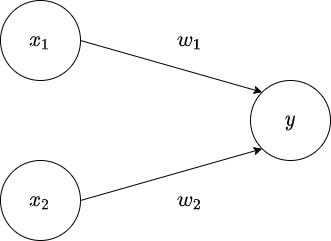
\includegraphics[width=0.50\hsize, keepaspectratio]{images/drawio/pa-seputoron.png}
  \caption{2入力パーセプトロン}
  \label{fig:pa-septoron}
 \end{figure}

\begin{equation}
y= \left \{
\begin{array}{l}
0 (w_1x_1 + w_2x_2 \leq \theta)\\
1 (w_1x_1 + w_2x_2 > \theta)
\end{array}
\right.
\label{eq:pa-septoron}
\end{equation}

2入力パーセプトロンにて$x_1, x_2$は入力信号,$y$は出力信号,$w_1, w_2$は重みである.重みは入力信号に対する重要度であり,この値によって入力信号の値が上下する.入力に重みを乗算したものの総和(ここでは$w_1x_1 + w_2x_2$)が閾値である$\theta$を超えると,パーセプトロンは1を出力する.

パーセプトロンを説明するために,例としてANDゲートをパーセプトロンで表現する.ANDゲートの真理値表を表\ref{tb:and_gate}に示す.このANDゲートをパーセプトロンで表現するためには,適切な重みと閾値を定めればよい.ANDゲートを表現する$(w_1, w_2, \theta)$の組み合わせとして,例えば$(w_1, w_2, \theta) = (0.3, 0.3, 0.5)$や$(0.1, 0.3, 0.35)$,$(1.0, 1.0, 1.0)$などが考えられる.

一つのパーセプトロン(単一パーセプトロン)では線形の表現しか行えない.このため,パーセプトロンは複雑な真理値表のゲートを表現することができないという致命的な問題があり,一般的な問題への適用には至らなかった.しかしながら,パーセプトロンの出力を次のパーセプトロンの入力にし,最終的な出力までに複数のパーセプトロンを重ねることで,非線形な表現を行うことが出来る.この方法は後に説明するニューラルネットワークにおける中間層にあたる.

\begin{table}[H]
  \centering
	\caption{ANDゲートの真理値表}
  \begin{tabular}{cc|c}
    $x_1$ & $x_2$ & $y$ \\ \hline
    0 & 0 & 0 \\ 
    1 & 0 & 0 \\
    0 & 1 & 0 \\
    1 & 1 & 1 \\
  \end{tabular}
  \label{tb:and_gate}
\end{table}


\subsection{ニューラルネットワーク}
ニューラルネットワークとは1986年にパーセプトロンの改良版として考案されたアルゴリズムである.パーセプトロンとニューラルネットワークとの違いは主に,単一パーセプトロンでは表現できないような非線形問題をニューラルネットワークでは表現できる点,そしてパーセプトロンでは人間の手によって適切に定められていた重みパラメータを,最適化手法により学習していく点である.

ニューラルネットワークのうち最も単純な構造である,3層ニューラルネットワークの概略図を図\ref{fig:3nn}に示す.円形で表現されているものはノードもしくはニューロンと呼ばれ,それぞれノードは固有の重みを持つ.また,一番左の列を入力層,一番右の列を出力層と呼ぶ.真ん中の列は隠れ層と呼ばれ,図\ref{fig:pa-septoron}のような単一パーセプトロンでは存在しなかった3番目の層が追加されたことにより,ニューラルネットワークは非線形問題のような複雑な問題を解決できるようになった.隠れ層は何層でも重ねることが出来るが,重ねれば重ねるほどに適切な重みを定めることが難しくなる.そこで適切な重みを定めるため考案されたアルゴリズムが,誤差逆伝搬法と呼ばれるものである.誤差逆伝搬法については2.4.2節で詳述する.

\begin{figure}[H]
 \centering
 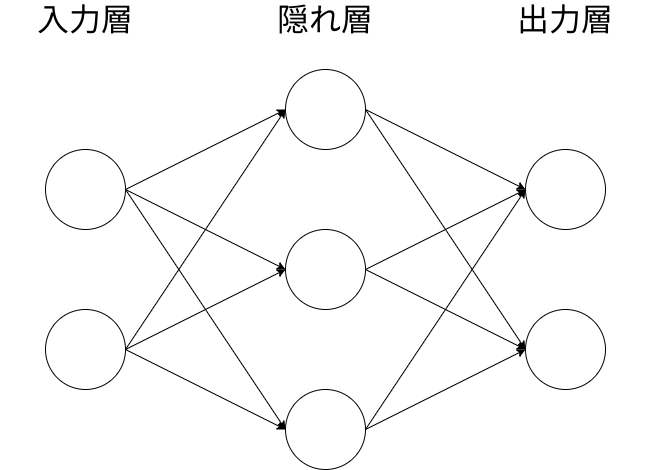
\includegraphics[width=0.7\hsize, keepaspectratio]{images/drawio/3nn.png}
 \caption{3層ニューラルネットワーク}
 \label{fig:3nn}
\end{figure}

\subsection{Deep Neural Network (DNN)}
DNNとはニューラルネットワークにおける隠れ層を多層化,すなわち層を深くしたものであり,現在深層学習と呼ばれているもの全般を指す.ニューラルネットワークにおける隠れ層はせいぜい2,3層であったが,現在使われているDNNではResNet\cite{He2016}のように150ほどの隠れ層をもつこともある.DNNのうち最も基本である全結合のニューラルネットワークでは,画像データを入力データにした際,一次元ベクトルに変換されて入力されてしまうため,画像内の形状やエッジなどの空間的特徴を捉えることが困難であるという課題があった.

\subsection{Convolutional Neural Network (CNN)}
CNNとは深層学習手法の一つであり,入力データの空間的特徴を捉えて学習を進めていくモデルである.CNNは主に画像認識や音声認識などに用いられる.代表的な学習済モデルとして,AlexNet\cite{Krizhevsky2012}やResNet\cite{He2016}などが存在する.CNNでは畳み込み演算とプーリングを用いることで,画像内の重要な空間的特徴を捉えて学習を進めることが可能である.

CNNでは一般的に畳み込み層とプーリング層が交互に続く形で特徴量抽出を行い,出力層の直前に全結合層で特徴量同士を結合させ判断,出力層で最終判断を行い予測を出力する.畳み込み層やプーリング層,それらの具体的な演算については2.2節で説明を行う.


\section{層の説明}
DNNにおけるモデルは様々な層で構成されている.それぞれの層には個別の役割があり,これらによって深層学習における特徴量抽出や予測が実現される.以下では主にCNNにて重要な層について,説明を行う.
\subsection{全結合層}
全結合層とは全ての入力データを入力し,1つの値を出力する層である.全結合層では,入力データのうち「正解の予測により必要なデータはどれか」を示す重みパラメータを学習し,予測の改善を行っていく.

\begin{equation}
 o = h(w_n i_n + b) (n = 1, 2, ... , 全データ数)
 \label{eq:affine}
\end{equation}

ここで,$i_n$は入力,$o$は出力,$w_n$は重み,$b$はバイアス項を指す.全結合層はいかなる種類のDNNにて広く用いられる層である.

式\ref{eq:affine}にて,$w_n i_n + b = x$と置き換えると,$o = h(x)$という関係になる.これは入力信号の総和が,$h(x)$という関数によって出力信号に変換されることを意味している.ニューラルネットワークにおいて,層の出力には$h(x)$のような関数が多くの場合存在し,これを\textbf{活性化関数}と呼ぶ.この活性化関数がパーセプトロンとニューラルネットワークとの違いの一つであり,またニューラルネットワークの表現力向上に大きく寄与している.活性化関数の詳しい説明は2.3節にて行う.
\subsection{畳み込み層}
畳み込み層は,入力データに対しフィルタを適用することで,入力データの特徴抽出を行う層である.畳み込み層において,重みはフィルタの値に相当する.

フィルタサイズ3x3の,畳み込み層における畳み込み演算の概略図を図\ref{fig:conv2d}に示す.畳み込み演算は画像処理におけるフィルター演算に相当し,行列同士の積和演算を行うことで入力データ内の特徴量抽出を果たしている.ここで,フィルタとの積和演算によって生成された行列を特徴マップと言う.

\begin{figure}[htbp]
 \centering
 
\includegraphics[width=0.9\hsize, keepaspectratio]{images/drawio/conv2d.png}
 \caption{畳み込み演算の概略図}
 \label{fig:conv2d}
\end{figure}

このように畳み込み演算を行うことで2次元データ内の空間的特徴抽出が行えるため,畳み込み層は画像分類問題などに適している.

\subsection{プーリング層}
プーリング層とはCNNにて畳み込み層と共に用いられる層であり,特徴の次元削減を行う層である.プーリング層は畳み込み層によって作成された特徴マップに対し,最大値を残す\textbf{最大プーリング},平均値を得る\textbf{平均プーリング}によって次元削減を行う.2x2の最大プーリングの概略図を図\ref{fig:maxpooling}に示す.

プーリング層の重要な役割として,
\begin{inparaenum}[(1)]
 \item 特徴マップの抽象化
 \item 特徴マップ内の平行移動に対して頑健(ロバスト)性を付与する
\end{inparaenum}
というものがある.(1)について,プーリング層は画像内の特徴を失わずに次元削減を行うことができる.つまり,画像内の重要な情報を保持したまま画像全体を抽象化出来る.この特性により,モデルにおいて層の浅い部分では画像内の細かな特徴を,層の深い部分では画像内の大まかな特徴を捉えることになり,結果としてプーリング層はモデルの判断基準の多様性向上に繋がっている.(2)について,入力データの小さなズレに対して,プーリング層は同じような結果を返す.すなわち,プーリング層はほぼ同じ形状をもつ(小さなズレのある)画像データにおいて,ズレを吸収する役割を持つ.これにより,モデルに局所パーツの回転・平行移動・スケールへの不変性を付与することが出来る.

\begin{figure}[H]
 \centering
 
\includegraphics[width=0.8\hsize, keepaspectratio]{images/drawio/maxpooling.png}
 \caption{2x2最大プーリングの概略図}
 \label{fig:maxpooling}
\end{figure}

\subsection{モデルの過学習とDropout層}
過学習(オーバーフィッティングとも呼ばれる)とは,学習データに対しモデルが適合しすぎた結果,テストデータに対するスコアが低くなってしまう現象を指す.過学習したモデルは学習データをほぼ完璧に正答することができるが,本来予測を行いたい対象である未知のデータに対しては,正しい予測を行えないことが多い.この未知データに対する予測性能は\textbf{汎化性能}と呼ばれ,深層学習分野にて重視される性能の一つである.

過学習が起こる原因としては,主に学習データの数が足りないこと,データに対してモデル構造が複雑すぎることなどが挙げられる.これに対し過学習を防ぐ方法は,主に学習データ数を増やすこと,モデルの複雑さを減らすこと,過学習が起きる直前で学習を止めること,そしてモデルの正則化を行うことなどが挙げられる.モデルの正則化とは,モデルが学習できる情報量に制限を掛けるものであり,これによってモデルの学習の量や質を制限し,汎化性能の向上を期待することが出来る.正則化手法で最も主要に扱われているものとして,Dropout\cite{Srivastava2014}が挙げられる.

Dropout層とは,深層学習モデルにDropoutをもたらす層である.
Dropout層の概略図を図\ref{fig:dropout}に示す.Dropout層が適用されると,ユーザーが指定した確率でモデル内のノードが無視されるようになる.これにより,モデルの汎化性能が向上する.
Dropoutによって汎化性能が上がる理由としては,\textbf{アンサンブル学習}と同様の効果が期待されるからである.アンサンブル学習とは複数のモデルを個別に学習させ,予測出力時にはそれらのモデルの出力の平均を用いるというものであり,これにより学習の性能が上がることが分かっている.Dropoutはノードをランダムに無効化するという処理により,一つのモデルを複数のより小さなモデルに分け,学習毎に毎回違うモデルを学習させる効果をもつ.この処理は,モデルに対しアンサンブル学習に近い挙動を取らせることが可能である.

\begin{figure}[H]
 \centering
 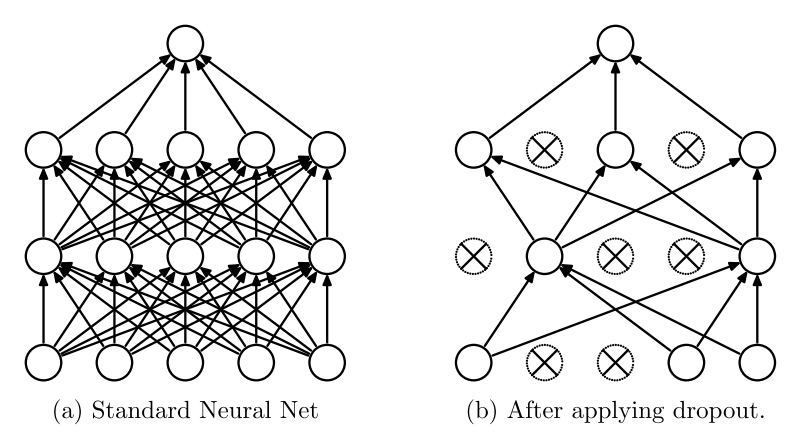
\includegraphics[width=0.8\hsize, keepaspectratio]{images/dropout.png}
 \caption{Dropout層の概略図\\\cite{Srivastava2014}より引用}
 \label{fig:dropout}
\end{figure}


\section{活性化関数}
活性化関数とは,ニューラルネットワークから導入された概念であり,各層におけるノード内の信号を出力信号に変換する関数である.ニューラルネットワークにおいて,多くの場合活性化関数は非線形である.これは,活性化関数に線形関数を用いると,ニューラルネットワークにおいて層を深くする意味がなくなるからである.線形関数をどんなに深く重ねても,これと同等の処理を持つ関数が非線形関数一つで表せるということが証明されている.これは,非線形関数を用いた場合,ネットワークの層を重ねることでモデルの表現力を大きく向上させられることを意味している.

あらゆる問題に適している活性化関数は今のところ発見されておらず,現在までに様々な活性化関数が考案されてきた.以下では代表例として,3つの活性化関数について述べる.
\subsubsection{sigmoid関数}
sigmoid関数は出力信号を0.0から1.0の範囲に押しとどめる働きをもつ,滑らかな形状をした関数である.
sigmoid関数の計算式を式\ref{eq:sigmoid}に示す.また,式\ref{eq:sigmoid}をグラフで表したものを図\ref{fig:sigmoid}に示す.
ニューラルネットワーク登場時には隠れ層に多く用いられていたが,
モデルを多層化した際に起こる勾配消失が問題になったことから,今では隠れ層にはあまり使われず,2値分類問題の出力層に使われることが多い.

\begin{equation}
 sigmoid(x) = \frac{1}{1 + e^{-x}}
 \label{eq:sigmoid}
\end{equation}

\begin{figure}[H]
 \centering
 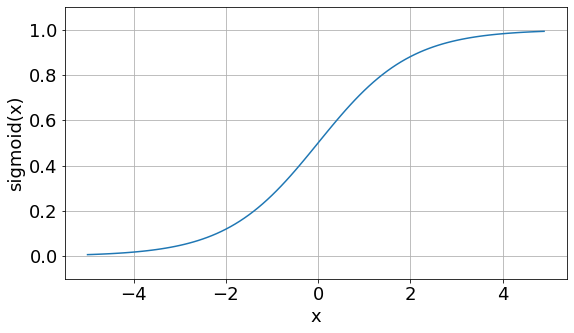
\includegraphics[width=0.7\hsize, keepaspectratio]{images/sigmoid.png}
 \caption{sigmoid関数}
 \label{fig:sigmoid}
\end{figure}

\subsubsection{ReLu関数}
ReLu関数\cite{Glorot2011}は,0以下の信号の場合出力は0とし,それ以上の信号の場合はそのまま出力する関数である.ReLu関数の計算式を式\ref{eq:relu}に示す.また,式\ref{eq:relu}をグラフで表したものを図\ref{fig:relu}に示す.ReLu関数はsigmoid関数を多層モデルの活性化関数に用いた際に生じる勾配消失問題を解決するために考案された活性化関数である.
% sigmoid関数の微分式が出力する最大値は0.25であるのに対し,ReLu関数の微分式の出力最大値は1である.sigmoid関数

\begin{equation}
  ReLu(x)= \left \{
  \begin{array}{l}
  x (x > 0)\\
  0 (x \leq 0)
  \end{array}
  \right.
  \label{eq:relu}
  \end{equation}

\begin{figure}[H]
  \centering
  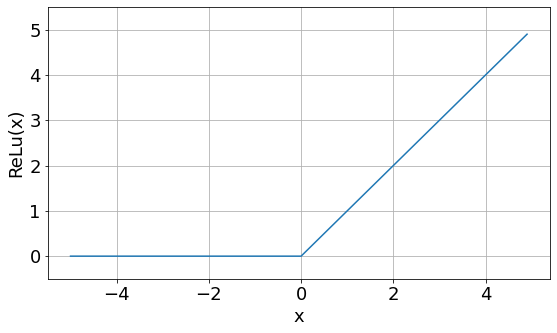
\includegraphics[width=0.7\hsize, keepaspectratio]{images/relu.png}
  \caption{ReLu関数}
  \label{fig:relu}
 \end{figure}

\subsubsection{softmax関数}
softmax関数は,多値分類問題の出力層に用いられる活性化関数であり,出力として「それぞれのラベルである確率」を導出する.$n$クラス問題において,最終層における$i$番目のユニットの出力を$x_{i}$とすると,softmax関数は式\ref{eq:softmax}のように定義される.

\begin{equation}
 y_{i} = \frac{e^{x_{i}}}{\sum_{k=0}^{n}e^{x_{k}}}
 \label{eq:softmax}
\end{equation}

\newpage
\section{損失関数と重み更新}
\subsection{損失関数}
深層学習モデルの学習の際に,パラメータをどのように更新するかを決めるのに用いられる指標を損失関数と呼ぶ.損失関数には様々な種類が存在し,解く問題の種類によって使い分ける.
一般的な損失関数として,式\ref{eq:mse}の主に回帰問題に使用される2乗平均誤差や,式\ref{eq:cee}の主に分類問題に使用されるクロスエントロピー誤差が挙げられる.式\ref{eq:mse}において,$y_{k}$はニューラルネットワークの出力,$t_{k}$は教師データを表す.また,式\ref{eq:cee}において,$y_{k}$はニューラルネットワークの出力,$t_{k}$は正解ラベルである.

\begin{equation}
	E = \frac{1}{2} \sum_{k} ({y_k} - t_k)^2
	\label{eq:mse}
\end{equation}

\begin{equation}
	E = -\sum_{k}t_{k}\log y_{k}
	\label{eq:cee}
\end{equation}

\subsection{重み更新}
ニューラルネットワークにおいてモデルの学習とは,モデルの予測が正解に近づくように各ノード内の重みやバイアスを更新していく作業のことである.深層学習においてモデルの学習は,教師データとモデルの予測データとの誤差を示す損失関数を最小化する(0にする)ように進める.以下では,深層学習モデルの学習の具体的な方法について説明する.
\subsubsection{誤差逆伝搬法}
誤差逆伝搬法とはニューラルネットワークでよく用いられる,ネットワーク全体に学習を行わせる,すなわちネットワーク全体の重み更新を行わせるための計算手法を指す.損失関数の数値はモデルの出力層で導出されるため,損失関数を指標にネットワーク全体の重み更新を行うには,出力層から入力層へと逆向きに重み更新を行っていく必要がある.これが誤差逆伝搬法の名前の由来である.

ここで,損失関数が0になるようにあるノードの重みを更新する時,損失関数の偏微分を用いる.これは微分がグラフの傾きを表すため,微分が正となる区間では重みを増加させ,負となる区間では重みを減少させればよいからである.誤差逆伝搬法では各ノードにおける損失関数の偏微分量を,合成関数の微分公式である\textbf{連鎖律}を用いて計算することで,膨大な計算量を省略している.
\subsubsection{勾配降下法}
誤差逆伝搬法がネットワーク全体の重み更新手法のことを指す一方で,最適化手法とは各ノードにてどのように重みを更新するかを決定するアルゴリズムを指す.数ある最適化手法の中で最も良く用いられる手法は勾配降下法であり,これはある一定数の訓練データごとに損失関数の全ての偏微分をまとめた\textbf{勾配}を導出し,また導出した勾配に基づいて重み更新を繰り返していくアルゴリズムである.重み$w$,およびバイアス$b$をもったノードに対する勾配降下法の計算式を式\ref{eq:gradient}に示す.ここで,$\eta$は\textbf{学習率}と呼ばれる勾配の更新量を決める定数であり,この値はユーザによって事前に定められる値である.また,勾配降下法における解探索のイメージを図\ref{fig:gradient}に示す.学習率は大きすぎると損失関数がいつまでも最小値にたどり着かず,また小さすぎると局所解から抜け出すことができなくなる.解く問題とモデルの構造によって最適な学習率は異なり,よって全てのモデルに適している学習率は存在しない.よりよい学習率の定め方は様々模索されており,Adam\cite{Kingma2015}のように最適化手法側で学習率を自動調整するような手法も存在する.
% 図\ref{fig:gradient}を例とすると,学習率が大きすぎる場合は最小値


\begin{equation}
  \begin{array}{l}
    w_{t+1} = w_t - \eta \frac{\partial E}{\partial w} \\
    b_{t+1} = b_t - \eta \frac{\partial E}{\partial b}
  \end{array}
  \label{eq:gradient}
\end{equation}

\begin{figure}[H]
 \centering
 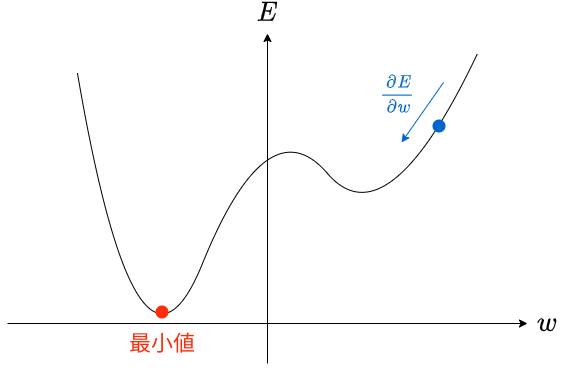
\includegraphics[width=0.7\hsize, keepaspectratio]{images/drawio/gradient.png}
 \caption{勾配降下法の解探索イメージ}
 \label{fig:gradient}
\end{figure}





\newpage
\chapter{使用するデータセット}
\section{Sloan Digital Sky Survey(SDSS)}
SDSSとは,天文学史上最も重要なサーベイ観測プロジェクトの一つとも称される大規模プロジェクトである.このプロジェクトは全天の約1/4の天域において,天体の画像および分光データを取得し,天体カタログを作成することを目的としたものである.SDSSでの撮像・分光データ取得はCCDを搭載した地上望遠鏡によって行われる.SDSSの最初のプロジェクトであるSDSS-I\cite{York2000}は2000年から2008年まで行われ,また対象を銀河系や超新星に絞ったSDSS-II\cite{York2000}が2005年から2008年にSDSS-Iと並行して実施された.その後,太陽系外惑星調査や天の川銀河の構造および進化などに焦点を当てたSDSS-III\cite{Eisenstein2011}が2008年から2014年に,南天・北天からの銀河系探索などを目的としたSDSS-IV\cite{Blanton2017}が2014年から2020年に行われた.

Galaxy Zooによって銀河形態ラベル付けが為されたサーベイであるSDSS-IIにおいて,銀河撮像に用いられた測光フィルタはu, g, r, i, zの5つが存在する.各測光フィルタにて撮影された画像の波長平均値を表\ref{fig:dr7_filters}に示す.また,それぞれの測光フィルタのスループット曲線を図\ref{fig:filter_responces}に示す.図\ref{fig:filter_responces}において,横軸は光の波長を示すオングストローム,縦軸はフィルター応答を示している.

\begin{table}[htbp]
  \centering
	\caption{SDSS-IIにおける,銀河撮像に用いられた測光フィルタ一覧\\(https://classic.sdss.org/dr7/instruments/imager/index.html より引用)}
  \begin{tabular}{|c|c|c|c|c|}
		\hline
    u & g & r & i & z \\ \hline
    3551Å & 4686Å & 6165Å & 7481Å & 8931Å \\ \hline
  \end{tabular}
  \label{fig:dr7_filters}
\end{table}


\begin{figure}[H]
 \centering
 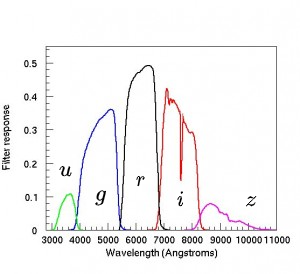
\includegraphics[width=11cm]{images/drawio/filter_responces.png}
 \caption{SDSS-IIにおける測光フィルタのスループット曲線\\(https://www.sdss.org/instruments/camera/ より引用)}
 \label{fig:filter_responces}
\end{figure}



\section{Galaxy Zoo (GZ)}
GZ\cite{Lintott2008}とは,人間の目による分類を行い銀河形態カタログを作成したプロジェクトである.従来の銀河形態分類は専門知識を持った天文学者のチームによって行われてきたが,SDSSのような何十万もの銀河が格納されたデータセットが登場するに従い,天文学者だけでは銀河データの増加に追いつけなくなってきた.このような状況を打破する方法として,インターネットを通じて専門知識を持たない有志の一般人に投票形式で形態分類を行わせる方法が提案された.これがGZである.

GZの最初の調査であるGalaxy Zoo 1\cite{Lintott2010}は2007年7月から2009年2月に行われた.Galaxy Zoo 1による調査の対象となった天体は,SDSSの測光パイプラインによって銀河の判定された天体,またはSDSSの分光観測に含まれていた天体のうち,スペクトルの性質から銀河に分類された天体であり,計893,212個の銀河がカタログに登録された.
Galaxy Zoo 1より詳細な形態分類を行うため,後継プロジェクトであるGalaxy Zoo 2\cite{Willett2013}が2009年2月から2010年4月まで行われた.詳細な形態分類を行うためには天体画像内の形態的特徴がよりはっきりしたものである必要があるため,Galaxy Zoo 2で取り扱った天体はSDSSの最も明るい約25\%の天体である,304,122天体であった.

Galaxy Zoo 1では,ウェブサイト\footnote{www.galaxyzoo.org}を通じて分類を集計した.サイトを訪れた有志の一般人はウェブサイトにて提示されたカラー銀河画像を見て,時計回り腕をもつ渦巻銀河・半時計回り腕を持つ渦巻銀河・エッジオン(地球から見ると幾何学的に薄い螺旋構造を真横に見る銀河)・楕円銀河・星もしくは分からない天体・マージャー(2つの銀河が衝突し合体している,合体銀河)の6つのうちいずれかに投票を行う.形態分類カタログは,対象となった銀河に対し,各形態分類の投票率を付与され作成される.本研究では,Galaxy Zoo 1で作成された銀河形態カタログから,渦巻銀河・楕円銀河・銀河形態の不確かな天体(以下,不確かな天体と呼称)の3つの分類ラベルを用いて,モデル学習を行う.

% Galaxy Zoo 1の後継プロジェクトであるGalaxy Zoo 2\cite{Willett2013}では,Galaxy Zoo 1より詳細な形態分類を行うため,決定木方式で形態分類を集計した.決定木は11個の分類タスクで構成されており,合計37個の分類が導かれる.各分類タスクは質問とそれに対する回答のセットで成り立っている.(このあと,GZ2の論文から引用した決定木のやつを貼る・それについて説明する)


\section{実験に使用するデータセットの作成方法}
\subsection{天体画像データ}
本研究分類モデル学習に用いる天体画像データとして,SDSS-IIにおけるデータリリースの中から,Data Release 7 (以下,DR7)\cite{Abazajian2009}より画像データを取得した.SDSS-IIにおけるデータリリースにはDR6とDR7が存在する.DR7はDR6の改良版であり,DR6では取得されていなかった天域の追加等が行われている.DR7では3億5700万天体の測光調査が行われた.
DR7 を選んだ理由としては,GZにおける銀河形態ラベル付けにDR7の銀河画像が用いられたからである.

DR7からの天体画像データ取得は,SDSSのData Archive Server(DAS)\footnote{http://das.sdss.org/www/html/das2.html}を介して行った.データベースから取得できるのは,$2048\times1489$ピクセルのある程度大きな天域の画像である.
この大きな画像には複数の銀河が含まれているため,そのままでは本研究で用いるCNNモデルの学習データに使用することはできない.
そのため,モデルの学習に用いるための天体画像を取得した場合,DASから取得した天域画像から対象天体の切り出しを行う必要がある.今回はGZにて形態ラベル付けが為されている銀河の中から15,000天体を対象に,銀河毎に$64\times64$ピクセルのサイズで切り出し処理を実行した.15,000天体を対象とした理由について,本研究では銀河の種類ごとに最大1,000天体をモデル学習およびテストに用いる.その際,楕円銀河を1,000天体以上確保できる数が15,000天体であったからである.

また,DR7から取得できる画像はu, g, r, i ,zの5つの帯域画像が存在する.その中から,今回の実験ではrフィルタから得られた帯域画像を使用した.rバンド画像を使用した理由としては,rフィルタが5つの測光フィルタのうち最も感度がよいからである(図\ref{fig:filter_responces}参照).測光フィルタの感度が高い程,より暗い光を捉えた画像が撮影される.よって,rバンド画像は5つの帯域画像のうち最も銀河の形態的特徴を捉えている可能性がある.

\subsection{形態分類ラベル}
今回分類モデル学習に用いる正解ラベルとして,Galaxy Zoo 1から取得できるTable2の分類フラグを用いた.
Table2はSDSS DR7に掲載されている天体のうち,分光スペクトルデータが観測されていた天体に関して収録されている.DR7における総天体数は3億5700万天体であり,Table2に収録されている天体数は667,944天体である.
この内先頭から15,000天体分を選びだし,本研究でのモデル学習およびテストに用いた.
なお,Table2全体における渦巻銀河・楕円銀河・不確かな天体の比率は0.285 : 0.093 : 0.622であり,銀河画像切り出しを行った15,000天体における比率は0.271 : 0.104 : 0.626 であった.
Table2の記載内容の一例を図\ref{fig:table2}に示す.

\begin{quote}
  \begin{itemize}
   \item SDSSにおける天体オブジェクトID (OBJID)
   \item 天体の天球座標 (RA, Dec)
   \item 投票数 (NVOTE)
   \item 各カテゴリの得票率 (P\_EL, P\_CW, P\_ACW, P\_EDGE, P\_DK, P\_MG)
   \item P\_CW, P\_ACW, P\_EDGEの合算にて導出された,渦巻銀河の投票率 (P\_CS)
   \item バイアスが除去された投票率 (P\_EL\_DEBIASED, P\_CS\_DEBIASED)
   \item 分類フラグ (SPIRAL, ELLIPTICAL, UNCERTAIN)
  \end{itemize}
\end{quote}

\begin{figure}[H]
  \centering
  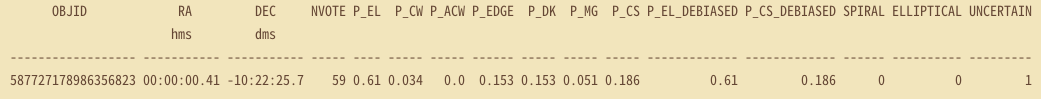
\includegraphics[width=1\hsize,keepaspectratio]{images/table2.png}
  \caption{Galaxy Zoo 1のtable2における一例}
  \label{fig:table2}
\end{figure}
 

バイアスが除去された投票率について説明を行う.
Bamford et al.(2009)\cite{Bamford2009}にて,遠方に存在する銀河は高い確率で楕円銀河に分類される傾向があることが報告された.これは,SDSSの空間解像度では遠方に存在する渦巻銀河の腕がはっきりと見えず,楕円銀河と誤認されてしまうからである.この形態分類のバイアスを分類バイアスと呼ぶ.Table2に記載されている''バイアスが除去された投票率''は,Banfordらによって提案されたバイアス補正方法を基に,分類バイアスを除去した投票率である.

分類フラグは,渦巻銀河・楕円銀河・不確かな天体の3つが存在する.渦巻銀河および楕円銀河の分類フラグは,分類バイアスの除去を行った得票率が8割を超えた場合に立つ.不確かな天体のフラグは,渦巻銀河および楕円銀河のフラグが立たなかった際に立つ.ここで,渦巻銀河(P\_CS)や楕円銀河(P\_EL)の投票率に関係がない,P\_DKやP\_MGの投票率が最も高い天体については不確かな天体にフラグが成立する.
今回はこの分類フラグを深層学習モデルの学習に用いる.なお,GZにはGalaxy Zoo 1とGalaxy Zoo 2の2つのプロジェクトが存在するが,本研究ではGalaxy Zoo 1の形態分類ラベルを実験に用いるため,今後はGalaxy Zoo 1をGZと呼称する.


\newpage
\chapter{SDSSとGalaxy Zooを用いた分類モデル学習}
この章では本研究の実験に用いられるデータセットであるSDSSとGZにて,学習データとテストデータの解像度が揃っているという条件のもと,どの程度の精度の分類モデルを作成することができるかを確認した.

本研究の将来展望は,高空間分解能観測装置データを用いてモデル学習を行うことで,既存の低空間分解能データセットに対し更なる高精度形態分類を提供するというものである.この将来展望にまつわる実験の最も初段階の前提条件として,まずは学習データとテストデータの解像度が揃っている条件にて学習する銀河形態分類モデルの精度がどのくらいであるかを検証する必要がある.

\section{実験概要}
第4章ではSDSSから取得した銀河画像とGZから取得した分類フラグを学習データとし,渦巻銀河・楕円銀河・不確かな天体のいずれかを予測する分類モデルを学習する.

\subsubsection{用いるデータセット}
実験で用いる天体画像データを作成するため,第3章で説明を行った15,000天体に対し,画像切り出し処理を実行した.その結果,GZにて渦巻銀河とラベル付けがされている天体のうち1天体,および不確かな天体1天体について切り出し処理が正常に行えなかった.切り出し処理の結果として,渦巻銀河4,057天体,楕円銀河1,561天体,不確かな天体9,380天体の計14,998天体を取得した.
14,998天体の赤方偏移別の個数を示したグラフを図\ref{fig:z_15000}に示す.
ここで赤方偏移とは,地球と対象天体が物理的に遠ざかっている場合や宇宙膨張などにより天体の発する光の波長が伸び,その結果光が赤い方向にずれる現象のこと,あるいはそのずれの大きさを数値化したパラメータのことを指す.
本研究では赤方偏移を後者の意味で用いる.一般的に赤方偏移の値が大きいほど,地球から遠い天体といえる.
渦巻銀河・楕円銀河・不確かな天体の切り出し画像の例を図\ref{fig:sdss_images_spiral}から図\ref{fig:sdss_images_uncertain}に示す.

\begin{figure}[H]
 \centering
 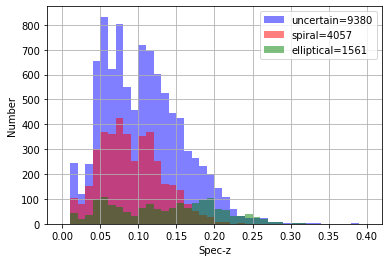
\includegraphics[width=1\hsize]{images/z_15000_0_040_kesson.png}
 \caption{切り出しを行えた14,998天体の分類ラベル別の個数グラフ}
 \label{fig:z_15000}
\end{figure}

\newpage
\begin{figure}[H]
 \centering
 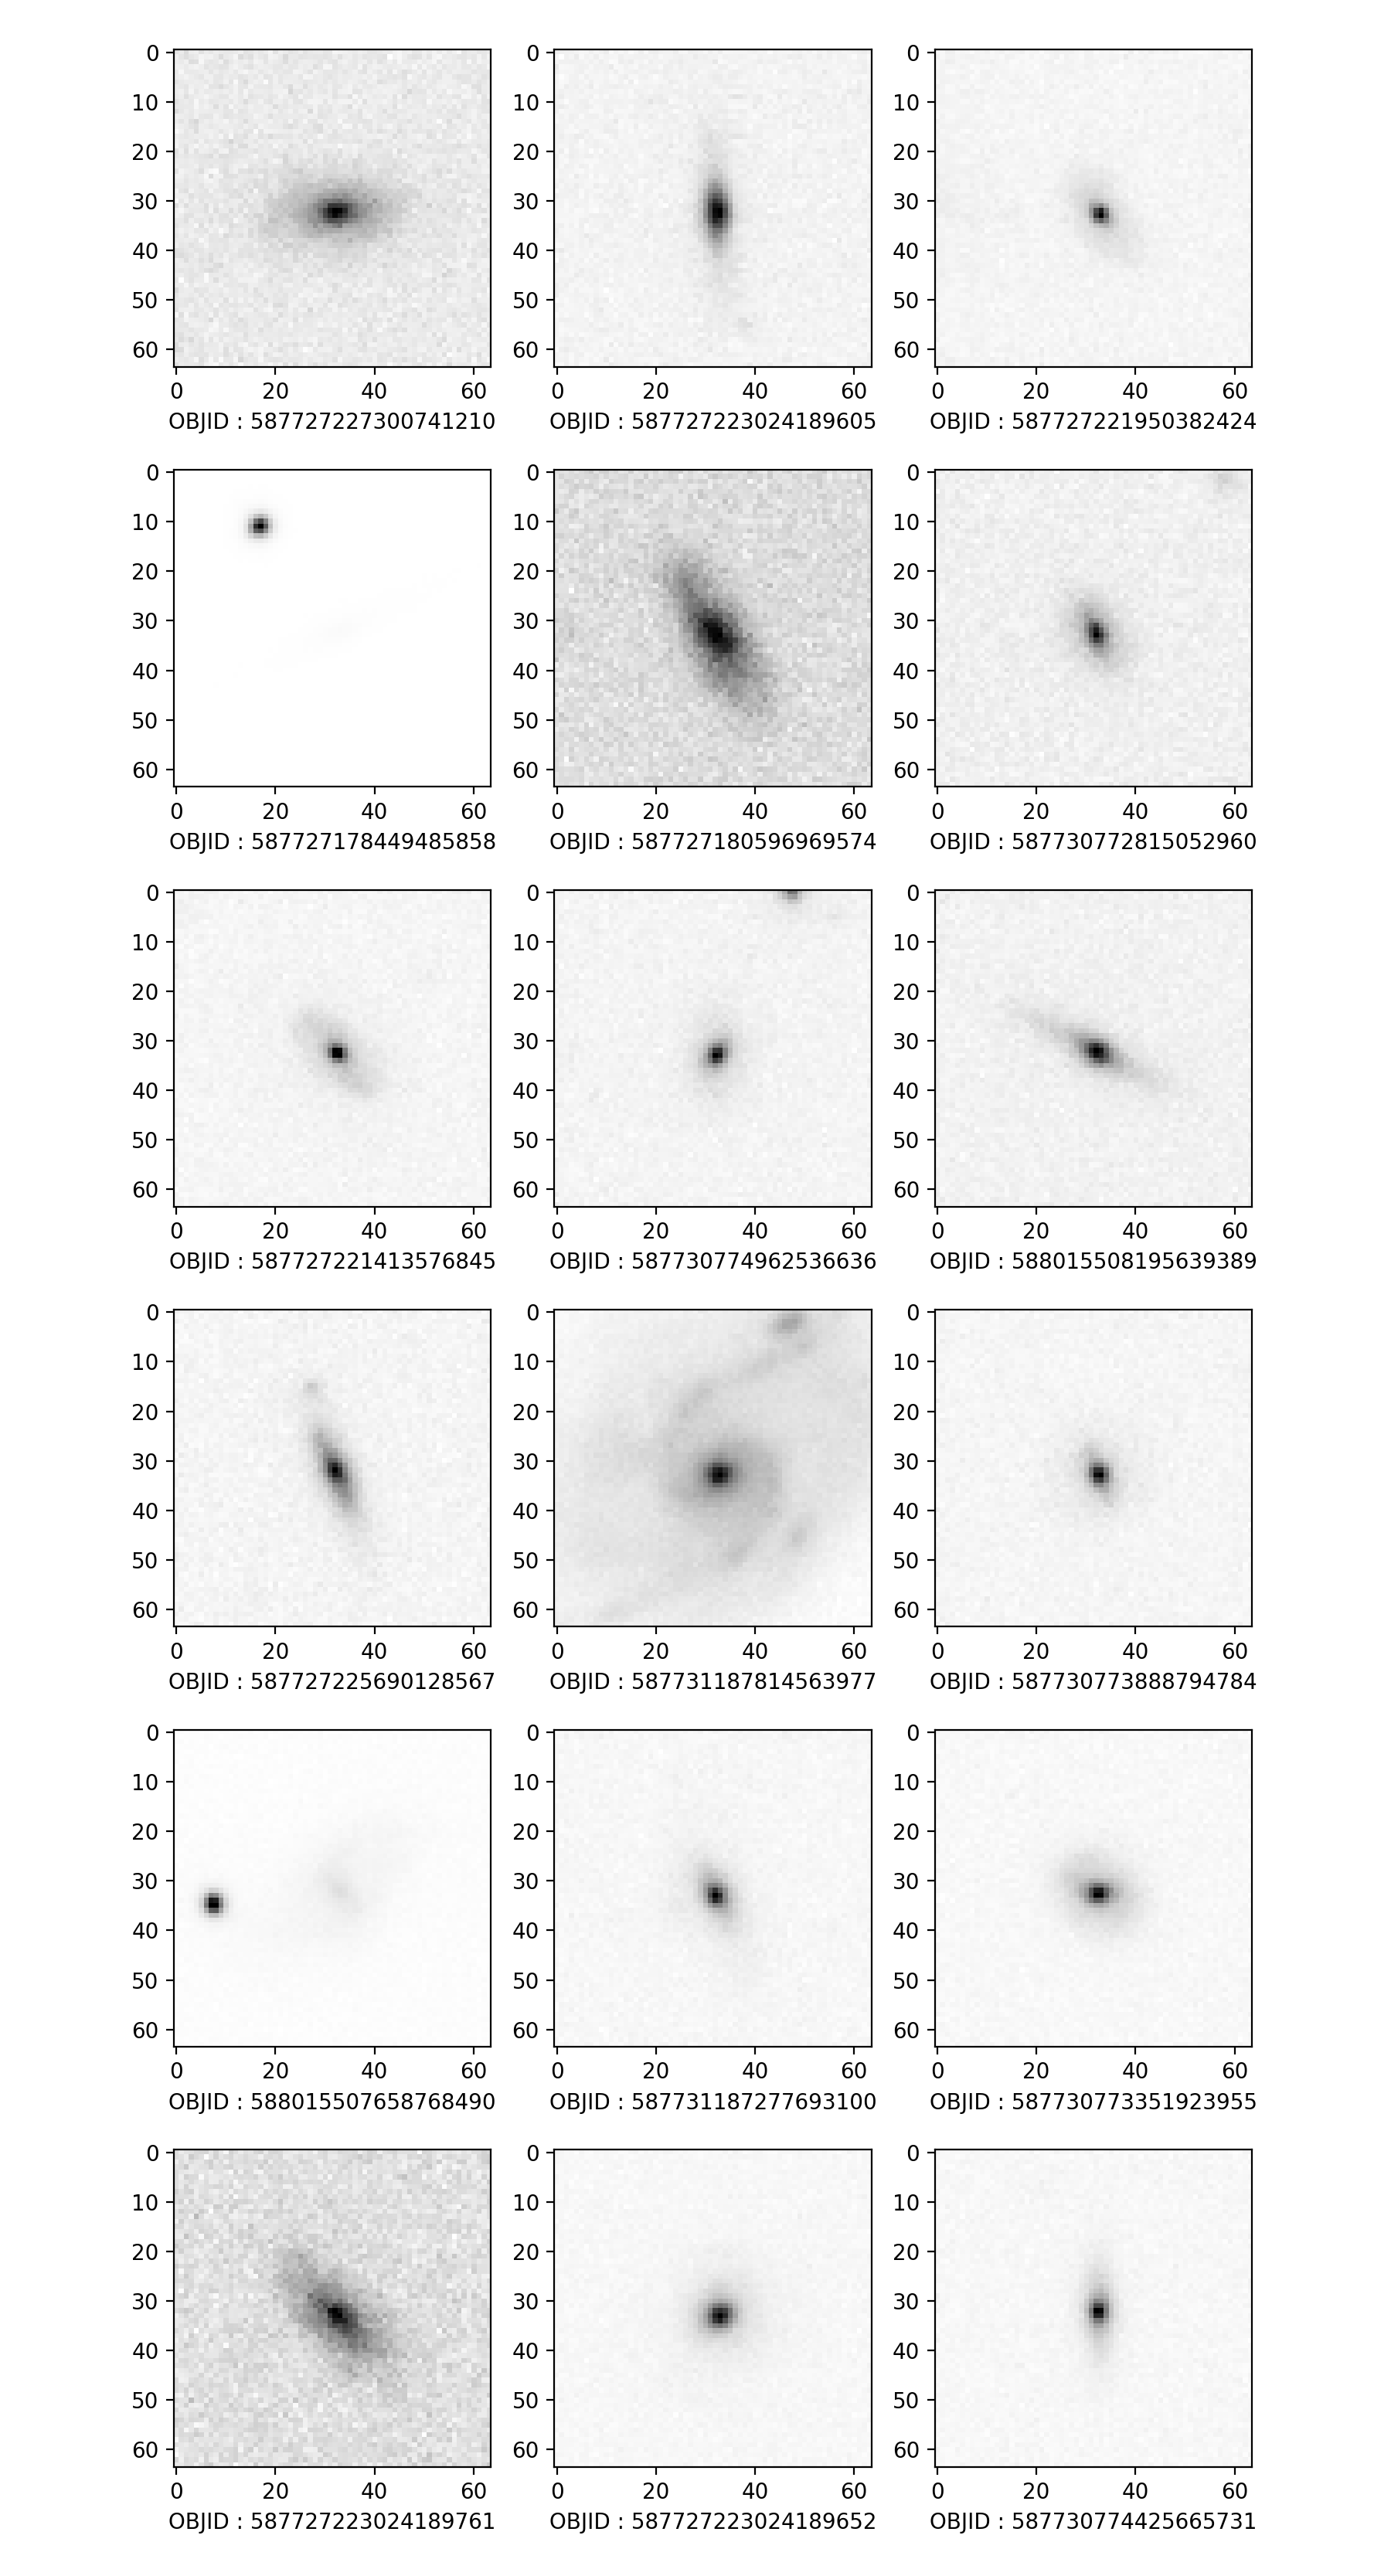
\includegraphics[width=0.5\vsize, keepaspectratio]{images/syuron_4syou_sdss_imgs/spiral_mini.png}
 \caption{渦巻銀河の切り出し画像の例}
 \label{fig:sdss_images_spiral}
\end{figure}

\newpage
\begin{figure}[H]
  \centering
  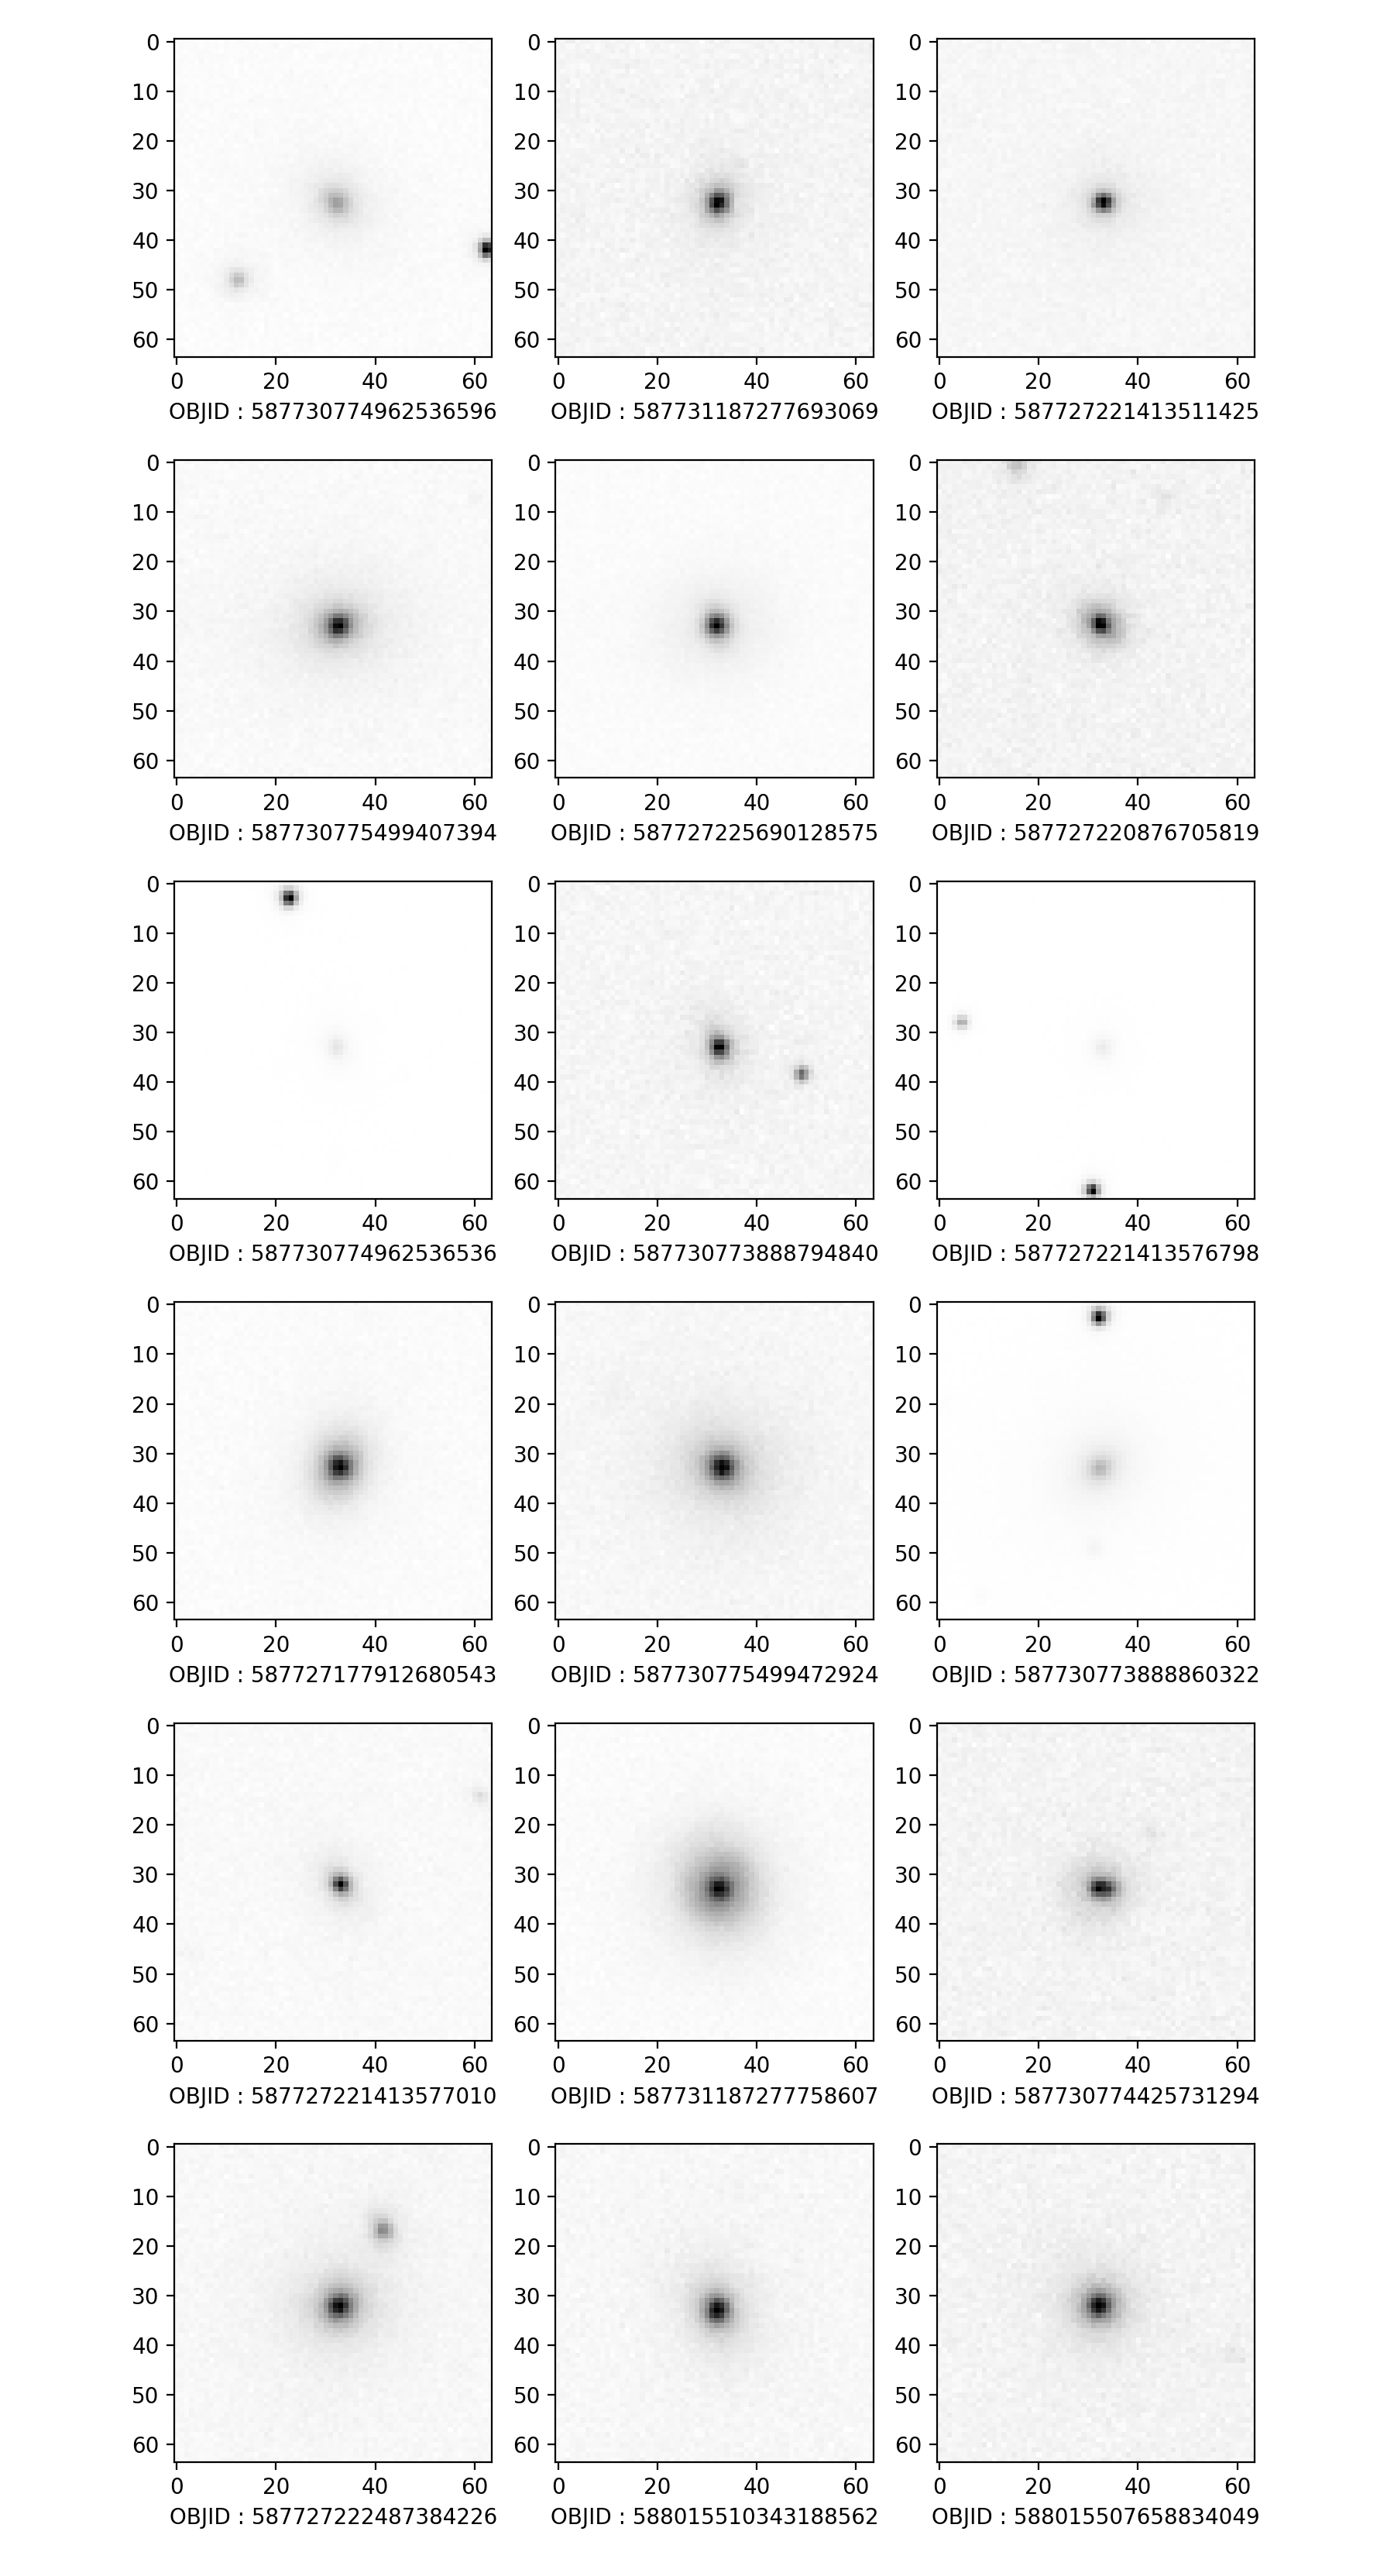
\includegraphics[width=0.5\vsize, keepaspectratio]{images/syuron_4syou_sdss_imgs/elliptical_mini.png}
  \caption{楕円銀河の切り出し画像の例}
  \label{fig:sdss_images_elliptical}
\end{figure}

\newpage
\begin{figure}[H]
  \centering
  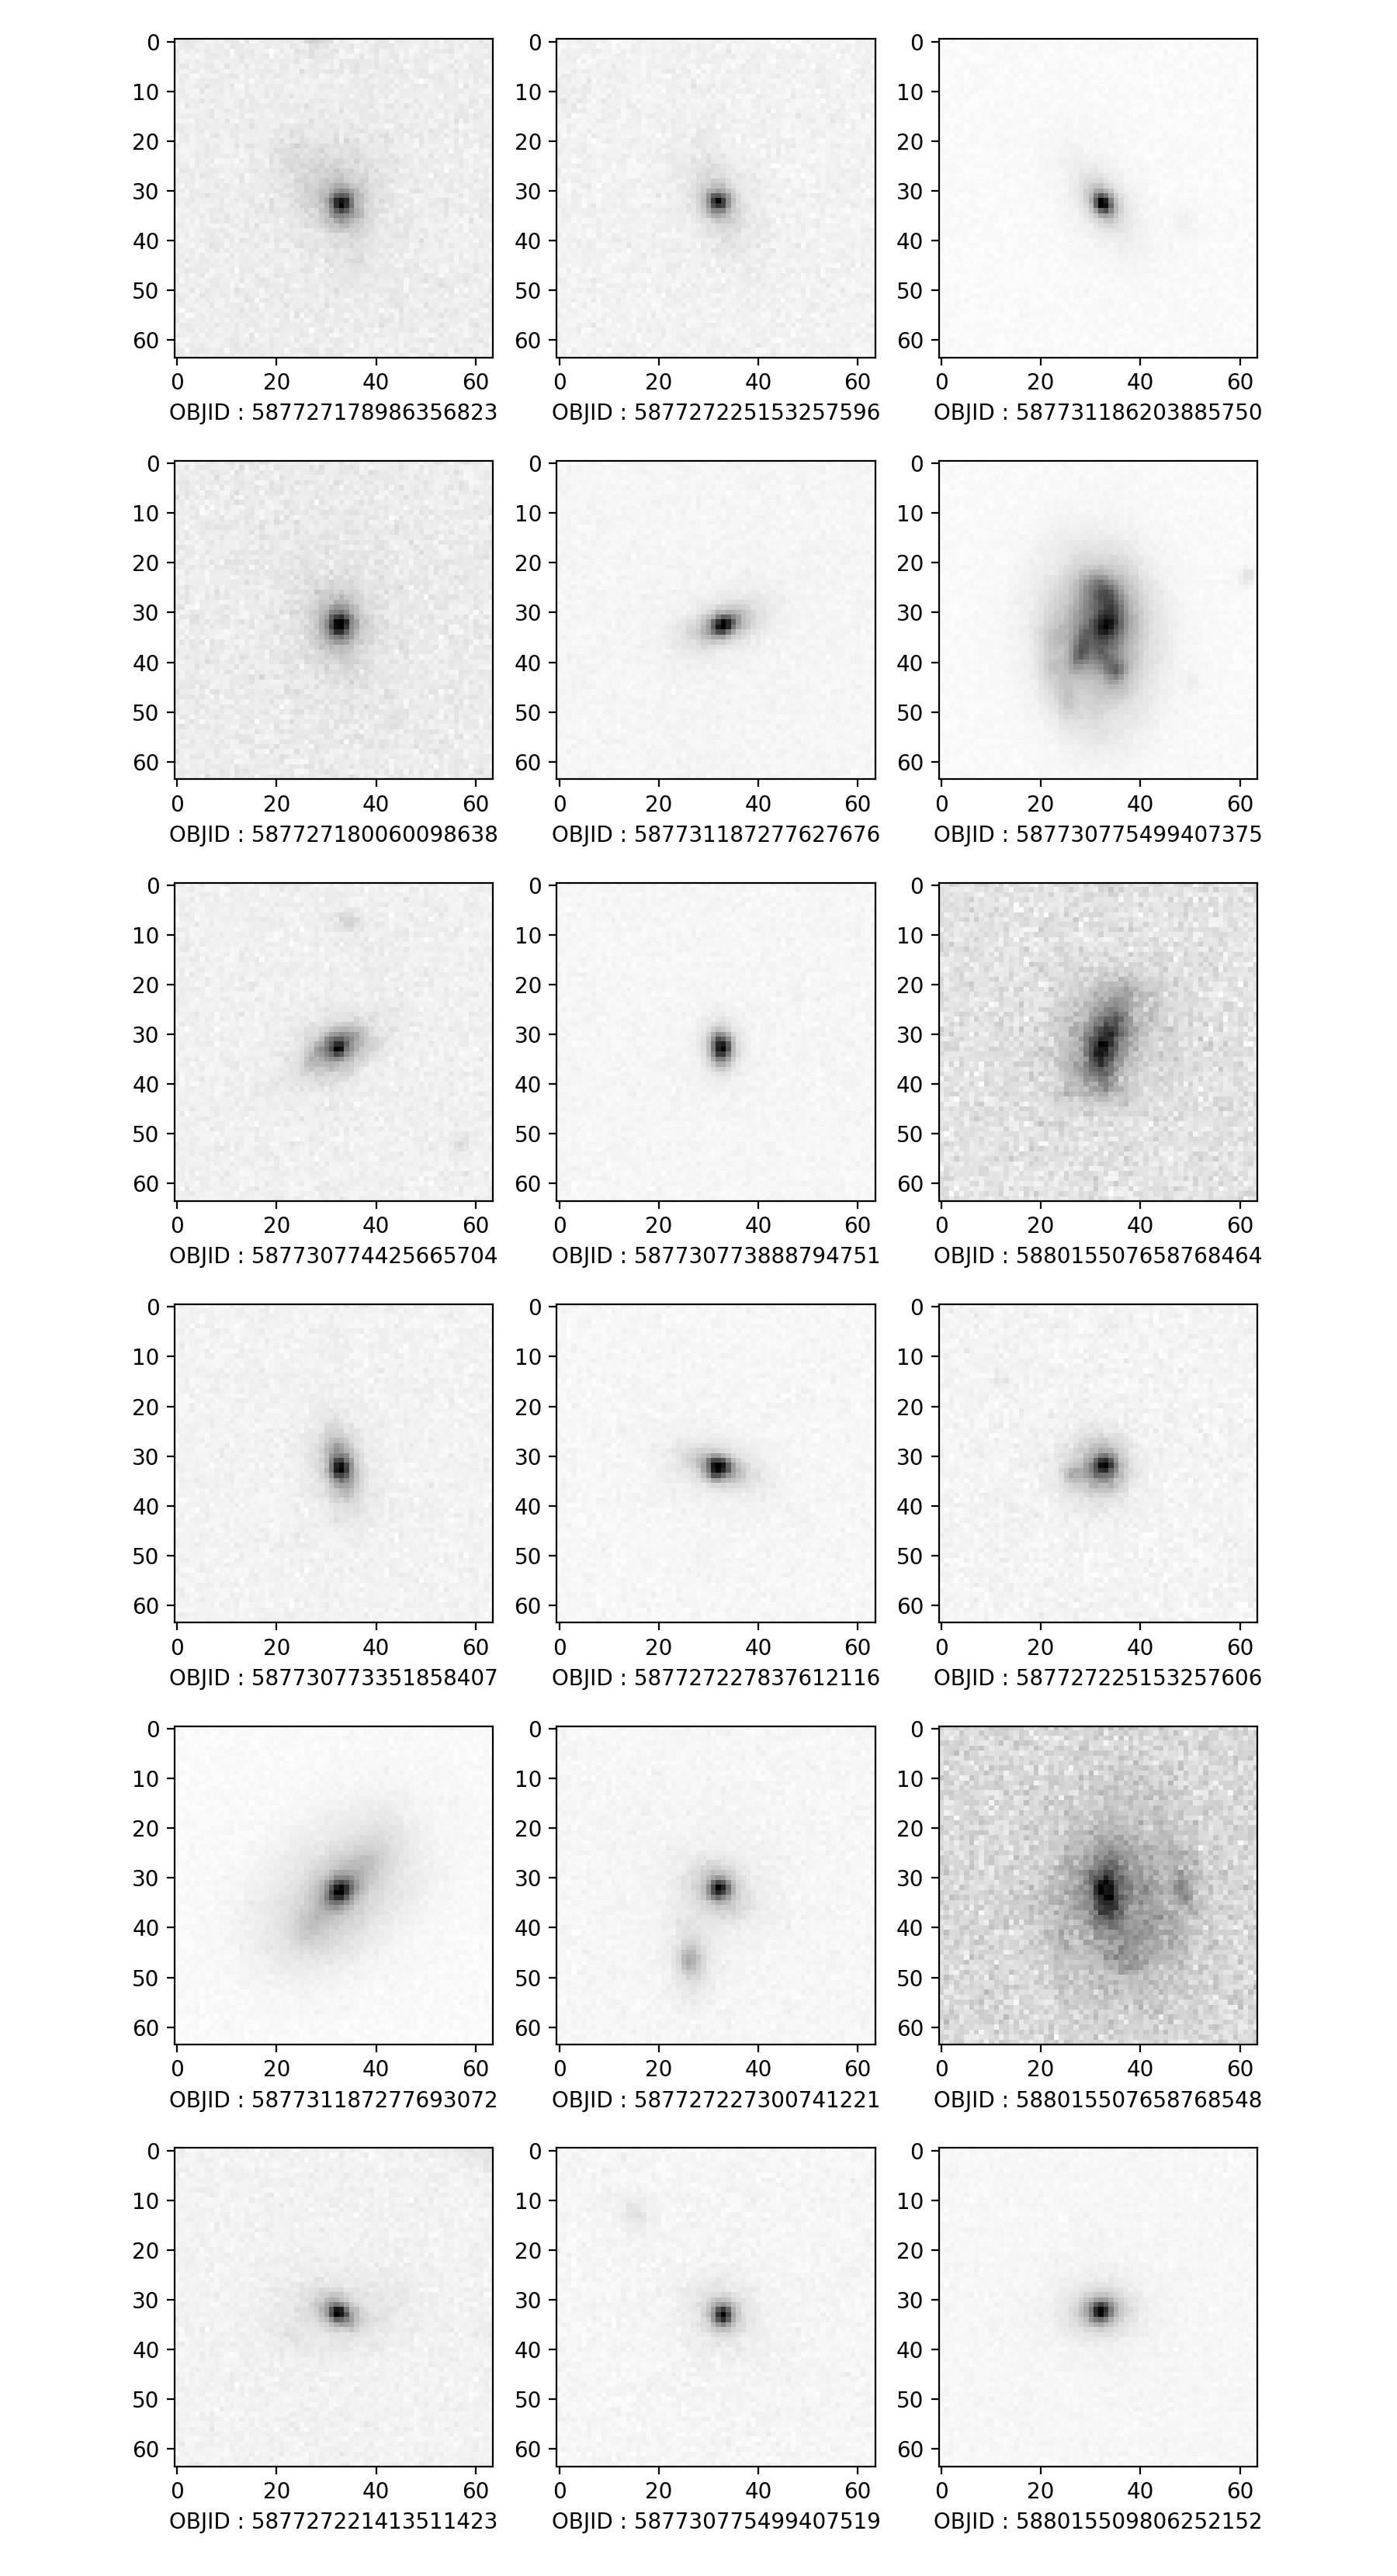
\includegraphics[width=0.5\vsize, keepaspectratio]{images/syuron_4syou_sdss_imgs/uncertain_mini.png}
  \caption{不確かな天体の切り出し画像の例}
  \label{fig:sdss_images_uncertain}
\end{figure}

\subsubsection{モデル構造}
今回用いた深層学習モデルは,Cheng et al.(2019)\cite{Cheng2019}にて用いられていた銀河形態分類モデルを参考にした.Cheng et al.を参考にした理由としては,モデルの学習に用いる形態分類ラベルに本研究と同じGZの形態分類ラベルを採用しており,99\%のaccuracyの分類モデルを作成しているからである.今回用いたモデルの構造を図\ref{fig:model_shape}に示す.このモデルは畳み込み層を合計3つ有しており,それぞれのカーネルサイズは3x3, 3x3, 2x2である.それぞれの畳み込み層の後には,2x2のmax-pooling層が存在する.全畳み込み層の後に全結合層が2層配置されており,それぞれ1024個のノードを有している.損失関数はカテゴリカルクロスエントロピーを使用した.また,モデルの最適化手法には確率的勾配降下法を使用し,バッチサイズは8とした.

\begin{figure}[h]
	\centering
	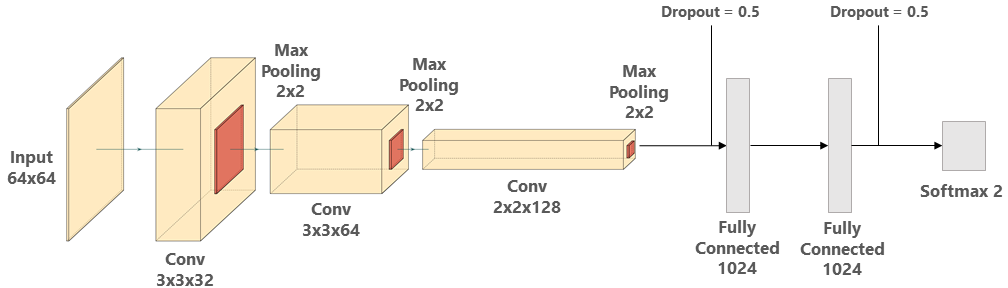
\includegraphics[width=14cm]{images/model_shape.png}
	\caption{用いた分類モデルの構造図}
	\label{fig:model_shape}
\end{figure}
 
\subsubsection{モデルの評価方法}
分類モデルの評価指標として,主にaccuracy (正解率)とtrue positive rate (真陽性率)を用いた.accuracyは全テストデータの中で正しく分類できたデータがどれだけあるかというものであり,モデルの正確性を表す指標である.true positive rateは本来陽性だと分類すべき全データのうち,どれほど正しく分類できたかを表す指標である.accuracyはモデル全体の正確性を表す指標だが,ラベル毎に予測の正確性を判断することはできないため,true positive rateも評価指標として採用している.

以下に2値分類問題を例とした場合の混同行列,accuracy, true positive rateの導出方法を示す.ここで混同行列とは,分類問題においてモデルが予測した値および真の値を行列形式で表したものであり,行成分がモデルによる予測ラベル,列成分がテストデータの真のラベルである.混同行列は分類モデルの性能を可視化・評価するのによく用いられ,モデルの予測値と真の値が交差する対角成分における数が多いほど,モデルが正確な予測を行っているといえる.

\begin{figure}[H]
 \centering
 
\includegraphics[width=12cm]{images/cm.png}
 \caption{2値分類問題における混同行列}
 \label{fig:cm}
\end{figure}

\begin{equation}
 accuracy = \frac{TP + TN}{TP + FP + FN + TN}
 \label{equ:accuracy}
\end{equation}

\begin{equation}
 true positive rate = \frac{TP}{TP + FN}
 \label{}
\end{equation}

\section{不確かラベルが与える分類精度への影響}
GZが与える形態分類フラグのうち「不確かな天体」というフラグが立っている天体は,渦巻銀河・楕円銀河のどちらの得票率も8割を超えなかった天体である.これらの天体は人間の目による形態分類が比較的難しい天体,つまり天体画像から読み取れる形態的特徴があいまいな天体であると考えられる.

この節では特徴があいまいだと考えられる不確かな天体群が,形態分類モデルの分類精度に与える影響を調べる.具体的には,不確かを含めた渦巻銀河・楕円銀河・不確かな天体の3種類を用いて学習およびテストを行うモデルと,不確かを除いた渦巻銀河・楕円銀河の2種類を用いて学習およびテストを行うモデルをそれぞれ作成し,テストデータに対する予測のaccuracyや混同行列の比較をする.そして不確かな天体の特性や学習に用いた際に分類精度に与える影響を調べる.

\subsection{実験条件}
モデルの学習およびテストを行う天体数は1,000天体とした.使用する天体は,切り出しを行えた14,998天体(図\ref{fig:z_15000}参照)からランダムに取得を行う.取得を行う際,赤方偏移$z$について,$0 < z < 0.2$という条件を設定し,あてはまらない天体は除外を行う.これは,地球との距離が遠すぎる天体を撮影した際,撮影された天体画像は銀河の形態的特徴が上手く捉えられていないことが多く,そのためそれらの画像をモデル学習に用いた場合,分類精度が低下する恐れがあるからである.使用天体を1,000天体取得したあと,学習データとテストデータの比率が7:3となるように切り分けを行った.なお本論文で行った実験の条件は今後特に述べない限り,取得する天体の赤方偏移$z$は$0 < z < 0.2$,学習データとテストデータへの切り分けの際の比率は7:3とする.

モデルの評価を行う際,モデルの学習およびテストを30回行い,accuracyの平均値および標準偏差を導出した.なお,30回の学習およびテストの際,学習実行毎に取得される天体は毎回シャッフルされる.
モデルの作成を複数回行う理由としては,深層学習モデルの最終的な分類精度はモデルの重みやバイアスパラメータの初期値依存性と,モデル学習ごとに毎回シャッフルされる使用データへの依存性をもつことから,モデル学習およびテストを複数回行うことでこれら2つの依存性によるモデル分類精度のばらつきを,平均値および標準偏差によって表すためである.


\subsection{実験結果}
不確かを含めた渦巻銀河・楕円銀河・不確かな天体の3値分類モデル,また不確かを除いた渦巻銀河・楕円銀河の2値分類モデルの学習およびテスト結果を
図\ref{fig:4_2_losses},図\ref{fig:4_2_accs}に示す.図\ref{fig:4_2_losses}は横軸epoch数・縦軸loss(損失関数)となっている.また,図\ref{fig:4_2_accs}は横軸epoch数・縦軸accuracy(正解率)となっている.
これらの図において,30回実行の平均値が実線,1標準偏差が透過で示されている.
また,青色のラインが学習データに対するスコア,黄色のラインがテストデータに対するスコアとなっている.lossのグラフについて,学習データに対する損失関数は学習が進むにつれ順当に下がっていくものの,ある一定のepochからテストデータに対する損失関数が上昇していく現象が見受けられる.この現象は\textbf{過学習}と呼ばれている.この現象が起こると,学習データに対し分類モデルが過剰に適合した結果,学習データに対する予測精度に比べテストデータに対する予測精度が低下していく.

また,不確かを含めた渦巻銀河・楕円銀河・不確かな天体の3値分類モデル,および不確かを除いた渦巻銀河・楕円銀河の2値分類モデルの,テストデータに対する予測結果を混同行列で表したものを図\ref{fig:4_2_cms}に示す.各セルにはそれぞれ個数の平均値と1標準偏差が示されている.また,個数の平均値によって各セルが色付けされており,色と個数平均値の対応は図右側のカラーバーによって示されている.


\begin{figure}[H]
 \centering
 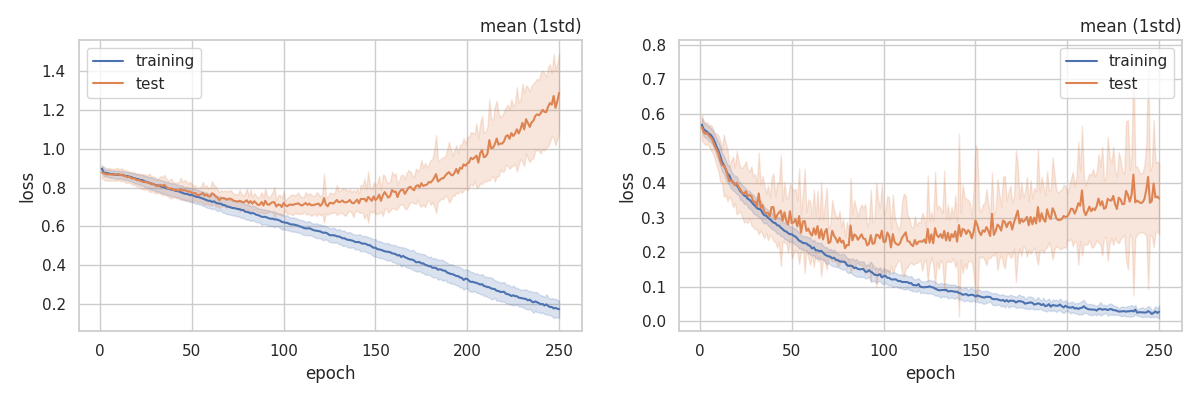
\includegraphics[width=1\hsize, keepaspectratio]{images/drawio/4_2_losses.png}
 \caption{loss関数の学習遷移 (左 : 3値分類 右 : 2値分類)}
 \label{fig:4_2_losses}
\end{figure}

\begin{figure}[H]
  \centering
  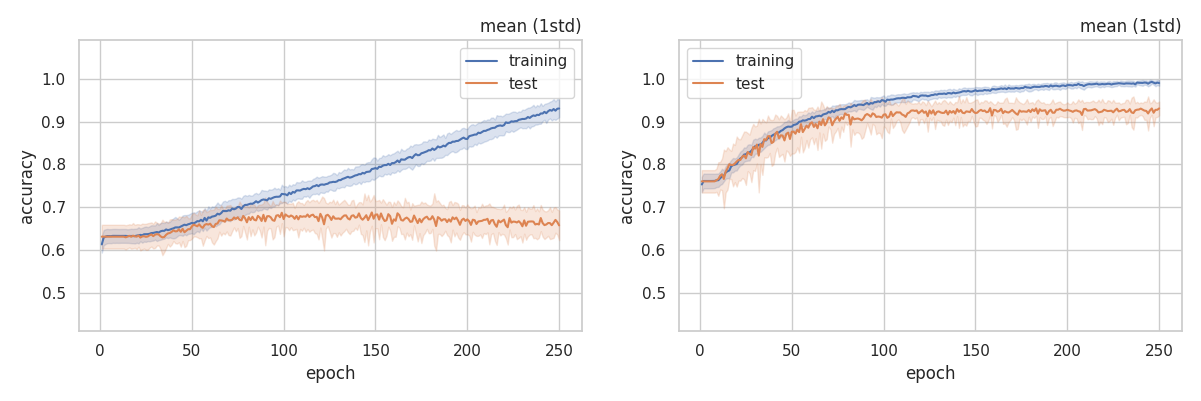
\includegraphics[width=1\hsize, keepaspectratio]{images/drawio/4_2_accs.png}
  \caption{accuracyの学習遷移 (左 : 3値分類 右 : 2値分類)}
  \label{fig:4_2_accs}
\end{figure}

\begin{figure}[H]
  \centering
  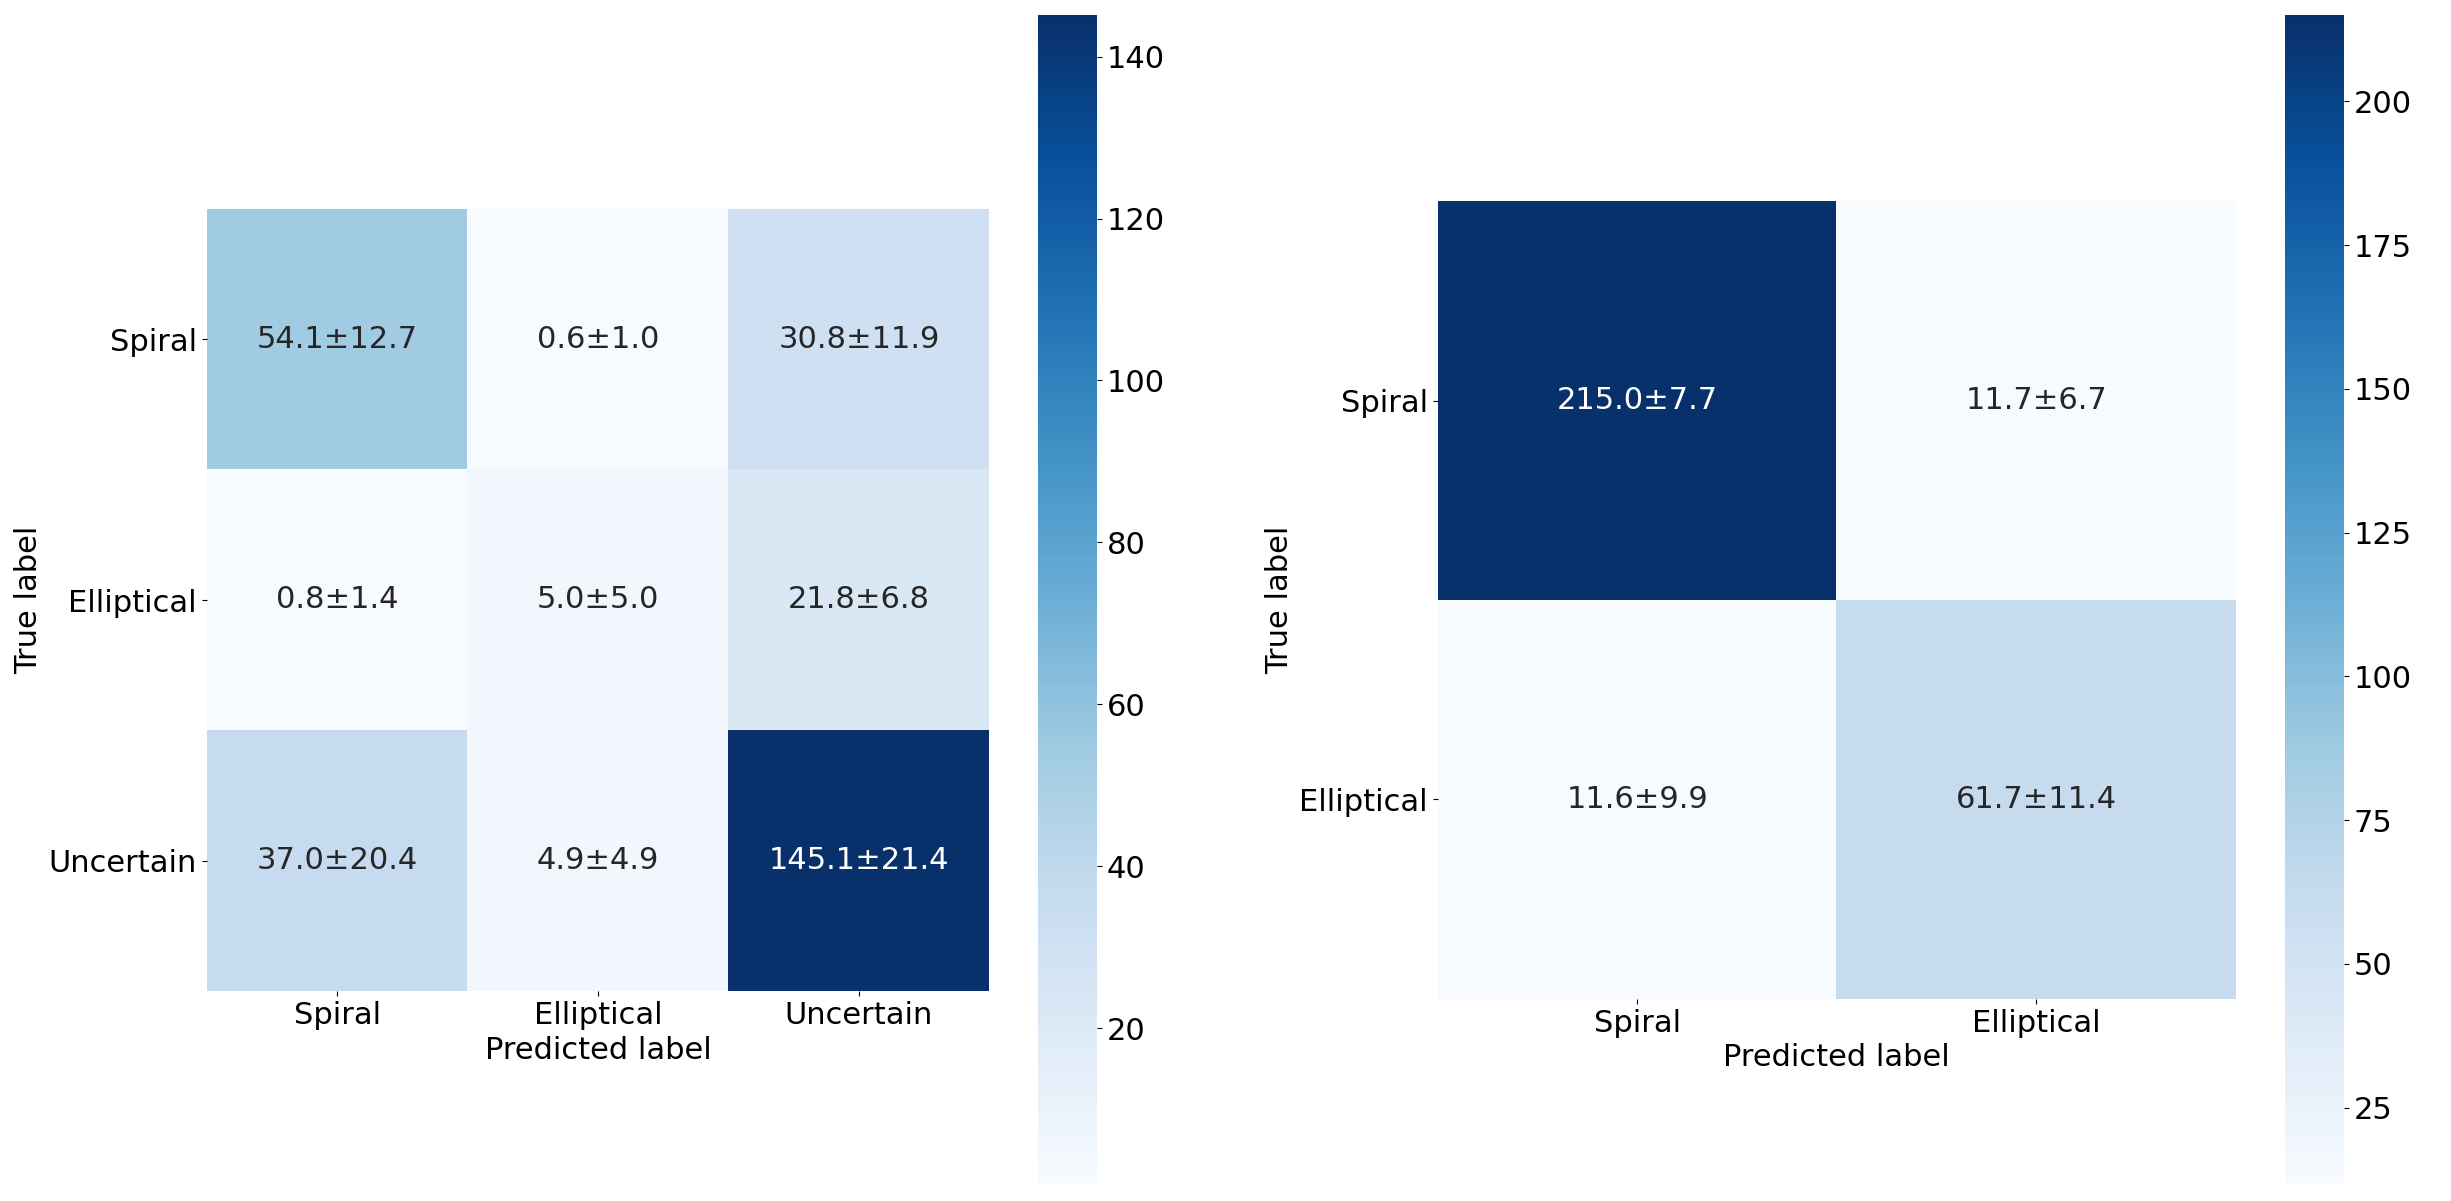
\includegraphics[width=1\hsize, keepaspectratio]{images/drawio/4_2_cms.png}
  \caption{混同行列 (左 : 3値分類 右 : 2値分類)}
  \label{fig:4_2_cms}
\end{figure}

% \begin{figure}[htbp]
%   \begin{minipage}[b]{0.45\hsize}
%     \centering
%     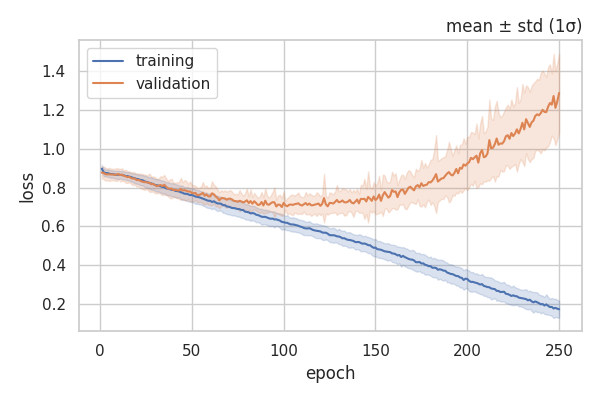
\includegraphics[keepaspectratio, width=7cm]{images/losses_ex4-1.png}
%     \caption{3値分類 : loss関数の学習遷移}
% 		\label{fig:losses_ex4-1}
%   \end{minipage}
%   \begin{minipage}[b]{0.45\hsize}
%     \centering
%     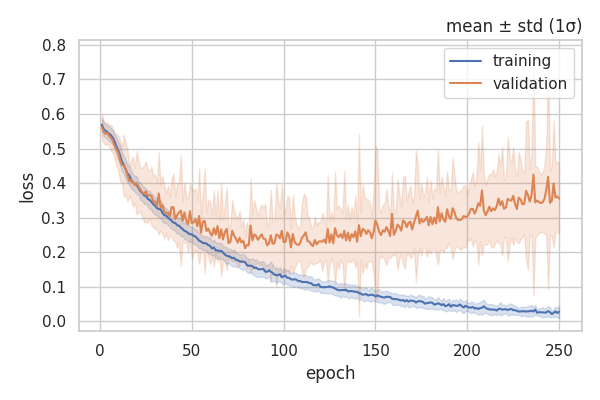
\includegraphics[keepaspectratio, width=7cm]{images/losses_ex4-2.png}
%     \caption{2値分類 : loss関数の学習遷移}
% 		\label{fig:losses_ex4-2}
%   \end{minipage}
% \end{figure}

% \begin{figure}[htbp]
%   \begin{minipage}[b]{0.45\hsize}
%     \centering
%     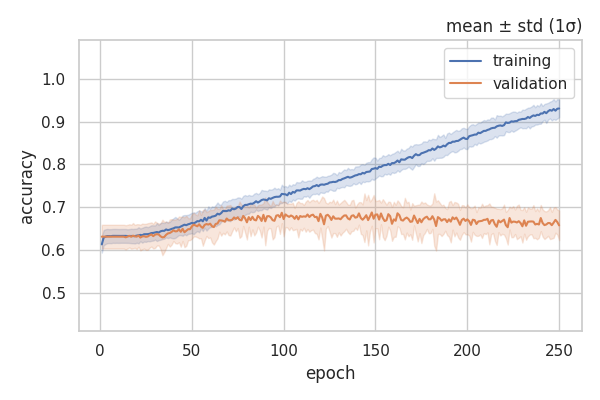
\includegraphics[keepaspectratio, width=7cm]{images/accs_ex4-1.png}
%     \caption{3値分類 : accuracyの学習遷移}
% 		\label{fig:accs_ex4-1}
%   \end{minipage}
%   \begin{minipage}[b]{0.45\hsize}
%     \centering
%     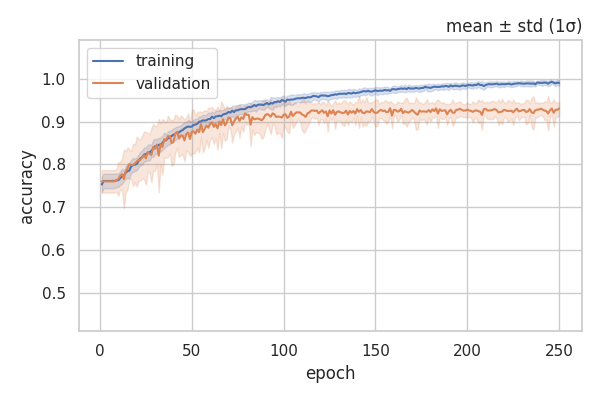
\includegraphics[keepaspectratio, width=7cm]{images/accs_ex4-2.png}
%     \caption{2値分類 : accuracyの学習遷移}
% 		\label{fig:accs_ex4-2}
%   \end{minipage}
% \end{figure}

% \newpage

% \begin{figure}[H]
%   \begin{minipage}[b]{0.45\hsize}
%     \centering
%     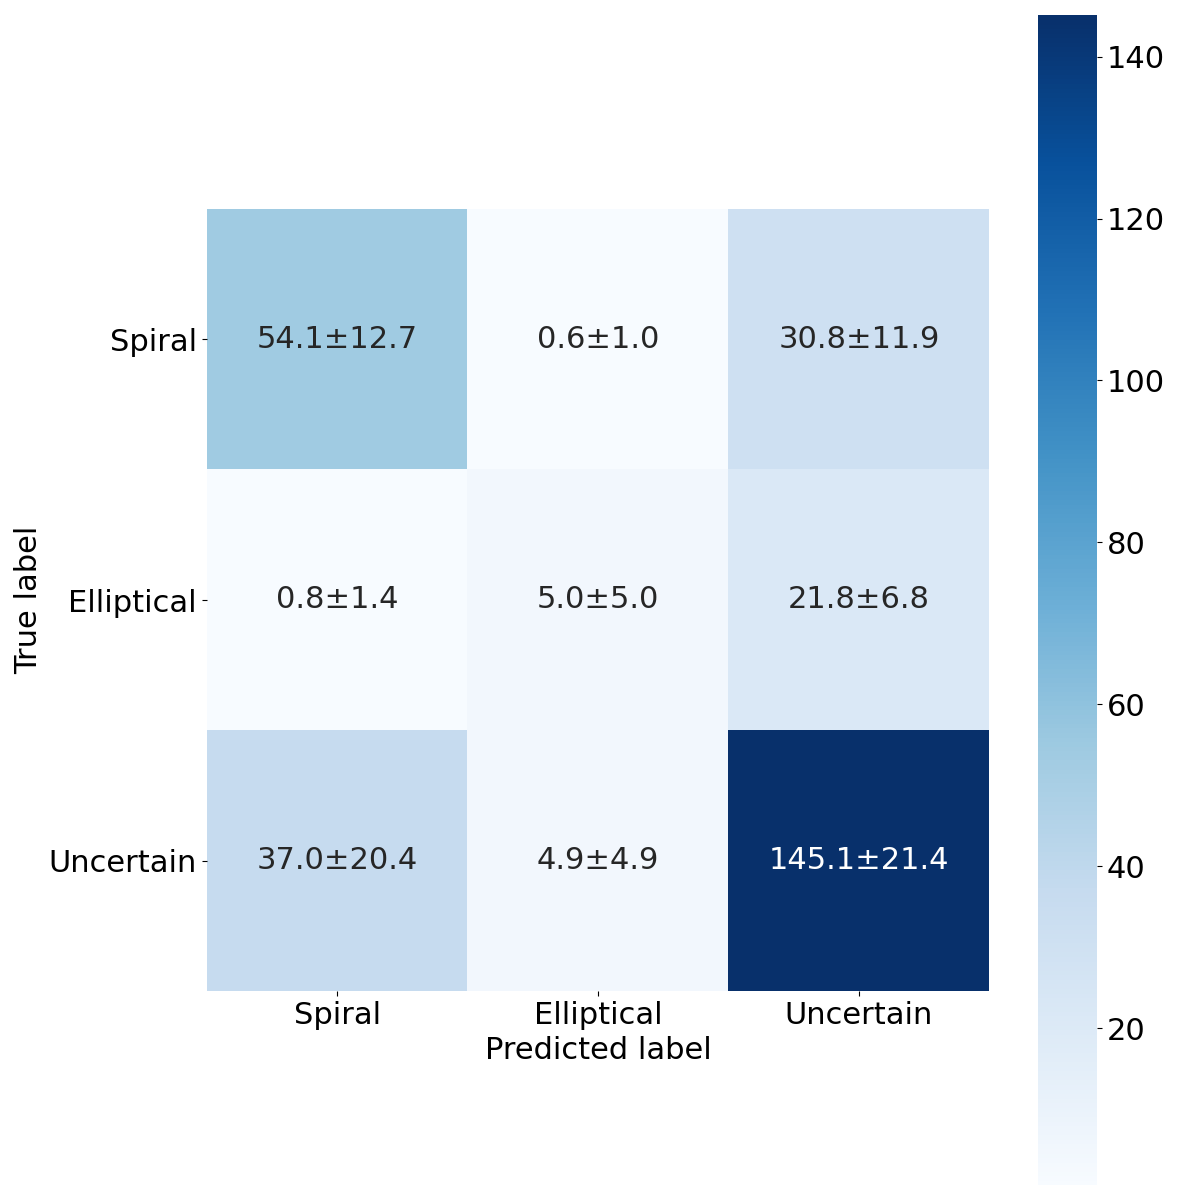
\includegraphics[keepaspectratio, width=7cm]{images/cm_mean_std_ex4-1.png}
%     \caption{3値分類 : 混同行列\\(平均$\pm$標準偏差(1$\sigma$))}
% 		\label{fig:cm_ex4-1}
%   \end{minipage}
%   \begin{minipage}[b]{0.45\hsize}
%     \centering
%     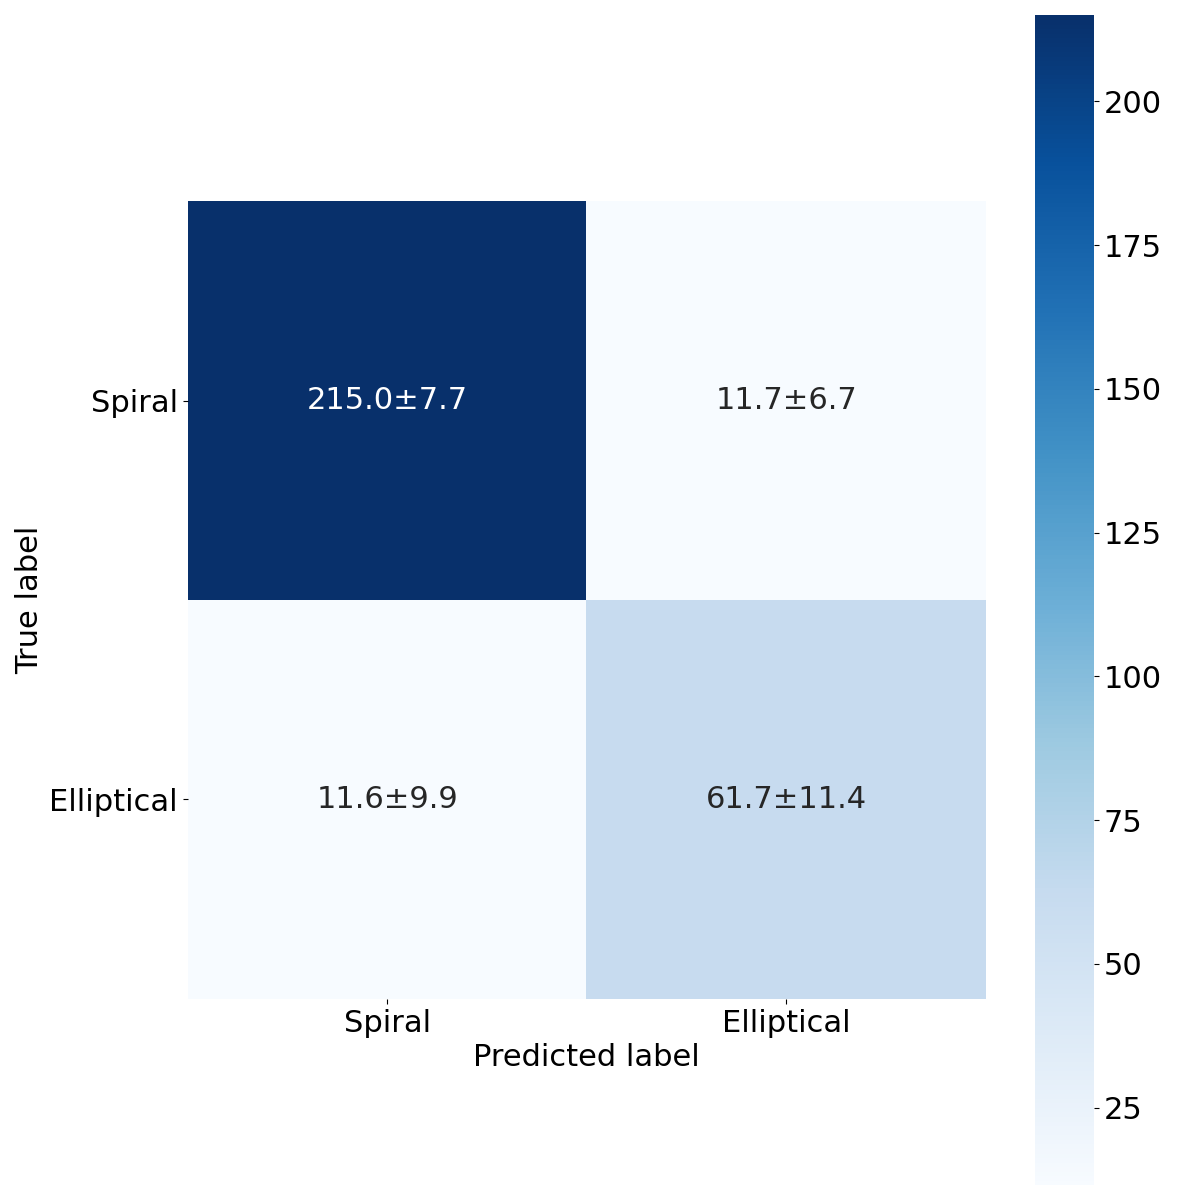
\includegraphics[keepaspectratio, width=7cm]{images/cm_mean_std_ex4-2.png}
%     \caption{2値分類 : 混同行列\\(平均$\pm$標準偏差(1$\sigma$))}
% 		\label{fig:cm_ex4-2}
%   \end{minipage}
% \end{figure}


% \subsubsection{モデル学習の進行}
% 図\ref{fig:losses_ex4-1}・図\ref{fig:accs_ex4-1}において,テストデータに対するスコアが100epoch付近までloss関数は降下,accuracyは上昇し,それ以降のepochではloss関数が上昇,accuracyが降下していることから,3値分類モデルでは100epochまで学習が良い方向に進んでいるもののそれ以降のepochからはモデルが学習データに対し過学習し,テストデータに対する汎化性能を失っていることが分かる.

% また図\ref{fig:losses_ex4-2}・図\ref{fig:accs_ex4-2}において,テストデータに対するスコアが100epoch付近までloss関数は降下,accuracyは上昇するものの,それ以降のepochではloss関数は上昇するがaccuracyは横ばいになっている.このことから,2値分類モデルにおいては100epoch目以降学習データに対し過適合はしているものの,テストデータに対する汎化性能は失っていないことが読み取れる.

\subsubsection{テストデータに対するaccuracyの評価}
モデルの形態分類性能を評価するため,両モデル間にてテストデータに対するaccuracyの比較を行う.性能評価においては,モデルが学習しきった際の分類性能を用いる.すなわち,accuracyを採るepoch数は,テストデータに対するaccuracyが最大となるepoch数とした.

不確かを含めた渦巻・楕円・不確かの3値分類モデル,および不確かを除いた渦巻・楕円の2値分類モデルにおける,テストデータへの予測精度(accuracy)を表\ref{tb:accs_4.2}に示す.3値分類・2値分類ともに,accuracyを採るepoch数を表内に示している.表\ref{tb:accs_4.2}には,今回の30回実行におけるaccuracyの平均値と標準偏差をそれぞれ1$\sigma$分記載した.

表\ref{tb:accs_4.2}より,標準偏差付き平均値において3値分類モデルと2値分類モデルとの間に有意な差があり,なおかつ2値分類モデルの方がaccuracyが高いことが分かる.

\begin{table}[htbp]
  \centering
	\caption{各モデルのテストデータに対する予測のaccuracy}
  \begin{tabular}{|c|c|}
		\hline
    & mean (1std) \\ \hline
    3値分類(渦巻・楕円・不確か) & $0.688 \pm 0.031$(148th epoch) \\ \hline
    2値分類(渦巻・楕円) & $0.931 \pm 0.017$(158th epoch) \\ \hline
  \end{tabular}
  \label{tb:accs_4.2}
\end{table}

\subsubsection{混同行列の導出方法,および両モデルにおける比較}
次に,混同行列を用いて各モデルのテストデータに対する予測精度の比較を行う.図\ref{fig:4_2_cms}より,3値分類モデルにおいて陽性を不確かな天体とした場合のtrue positive rateは$145.1/(37.0+4.9+145.1) = 0.776$だが,渦巻銀河群においては$54.1/(54.1+0.6+30.8) = 0.633$,楕円銀河群においては$5.0/(0.8+5.0+21.8) = 0.181$である.このことから,学習した3値分類モデルは不確かな天体群に比べ渦巻・楕円銀河を正しく分類する性能が劣っており,特に楕円銀河を正しく分類性能することができないことが読み取れる.
同じく図\ref{fig:4_2_cms}より,2値分類モデルにおいて陽性を渦巻銀河とした場合のtrue positive rateは$215.0/(215.0+11.7) = 0.948$,楕円銀河とした場合は$61.7/(11.6+61.7) = 0.842$であることが分かる.2つのモデルを比較すると,渦巻銀河と楕円銀河にまつわるtrue positive rateは3値分類モデルより2値分類モデルの方が高いことが分かる.true positive rateはラベル毎の予測の正確性を表す指標であることから,渦巻銀河および楕円銀河を正しく分類する性能は3値分類モデルよりも2値分類モデルの方が優れていることが分かる.

% また,図\ref{fig:cm_ex4-1},図\ref{fig:cm_ex4-2}より,3値分類モデルに用いたテストデータ内には不確かな天体群が約2/3存在し,また2値分類モデルに用いたテストデータ内には渦巻銀河と楕円銀河の比率がおおよそ3:1となっていることがわかる.これは今回用いる天体の母集団である15,000天体(図\ref{fig:z_15000}参照)の特性と一致している.


\newpage
\section{クラスインバランスの影響}
4.2節の図\ref{fig:4_2_cms}より,テストデータにおいて銀河形態ラベルのクラスインバランス(クラスの不均衡)が起きていることがわかった.このインバランスは今回のモデル学習・テストに用いている銀河の母集団(図\ref{fig:z_15000}参照)の性質と一致している.このことから,GZで銀河形態ラベル付けされている天体を深層学習モデルに用いる場合は,クラスインバランスを考慮せねばならず,またこのクラスインバランスがモデルの分類精度に与える影響を調べる必要がある.

この節では,学習データおよびテストデータ内の銀河形態ラベルのクラスインバランスが,形態分類モデルの分類精度に与える影響を調べる.
具体的にはモデルの学習およびテストに渦巻銀河・楕円銀河の比率が異なるインバランスドデータ(不均衡データ)を用いた場合と,渦巻銀河・楕円銀河の比率が等しいバランスドデータ(均衡データ)を用いた場合とで,テストデータに対する予測のaccuracy,true skill statistic(TSS)や混同行列の比較をする.true skill statisticについては\ref{sec:4-3-1}節にて説明を行う.

\subsection{実験条件}
\label{sec:4-3-1}
モデルの学習およびテストを行う天体の選定方法として,インバランスドデータにおいては切り出しを行えた14,998天体(図\ref{fig:z_15000}参照)のうち不確かな天体を除いた渦巻銀河4,057天体,楕円銀河1,561天体の計5,618天体から,ランダムに1,000天体の取得を行った.またバランスドデータにおいては渦巻銀河と楕円銀河の比率を等しくするために,不確かな天体を除いた計5,618天体から渦巻銀河を500天体,楕円銀河を500天体取得した.
またバランスドデータでは,学習データ・テストデータのどちらも渦巻銀河と楕円銀河の比率が等しくなるように1,000天体からの切り分けを行った.

モデルの性能評価は4.2節と同様の方法で行った.具体的には,モデルの学習およびテストを30回行い,accuracyの平均値および標準偏差を導出した.
なお,30回の学習およびテストの際,学習実行毎に取得される天体は毎回シャッフルされる.
また4.3節の実験においては,モデルの評価指標としてtrue skill statistic(以下,TSSと呼称)の導出も行った.ここでTSSとはaccuracyと同じく正確性を表す指標であるが,テストデータ内のデータインバランス性に対しロバストな性質がある.TSSの式を式\ref{equ:tss}に示す.

\begin{equation}
	TSS = \frac{TP}{TP + FN} - \frac{FP}{TN + FP}
 \label{equ:tss}
\end{equation}

TSSを用いた理由としては,インバランスドデータでのモデル学習・テストにおいて,30回実行における実行毎に取得する天体の渦巻銀河・楕円銀河の比率が毎回異なることから,accuracyだけでは銀河形態ラベルのクラスインバランスを正しく評価できないためである.そこでデータセット内の分類ラベルのインバランス性にロバストな性質をもつTSSも評価指標に加えている.

\subsection{実験結果}
渦巻銀河・楕円銀河の比率が異なるインバランスドデータで学習およびテストを行った2値分類モデル,また渦巻銀河・楕円銀河の比率が等しいバランスドデータで学習およびテストを行った2値分類モデルの学習結果を図\ref{fig:4_3_losses},図\ref{fig:4_3_accs}に示す.
また,両モデルのテストデータに対する予測結果を混同行列で表したものを図\ref{fig:4_3_cms}に示す.

図\ref{fig:4_3_losses}から図\ref{fig:4_3_cms}の構成は,4.2節における図\ref{fig:4_2_losses}から図\ref{fig:4_2_cms}と同様であり,最上段は横軸epoch数・縦軸loss(損失関数),中段は横軸epoch数・縦軸accuracy(正解率),最下段はテストデータに対する予測結果を混同行列で表したものである.


\begin{figure}[H]
  \centering
  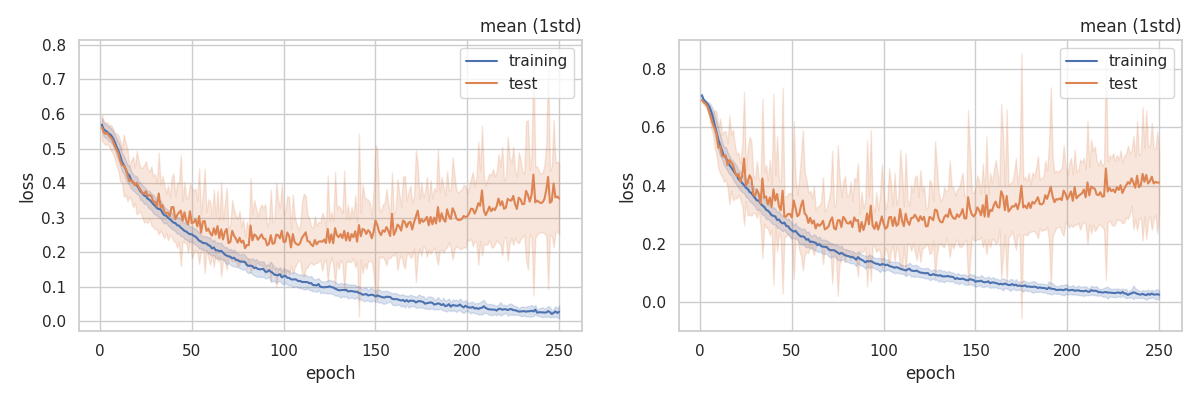
\includegraphics[width=1\hsize, keepaspectratio]{images/drawio/4_3_losses.png}
  \caption{loss関数の学習遷移\\(左 : インバランスドデータ 右 : バランスドデータ)}
  \label{fig:4_3_losses}
\end{figure}
 
\begin{figure}[H]
  \centering
  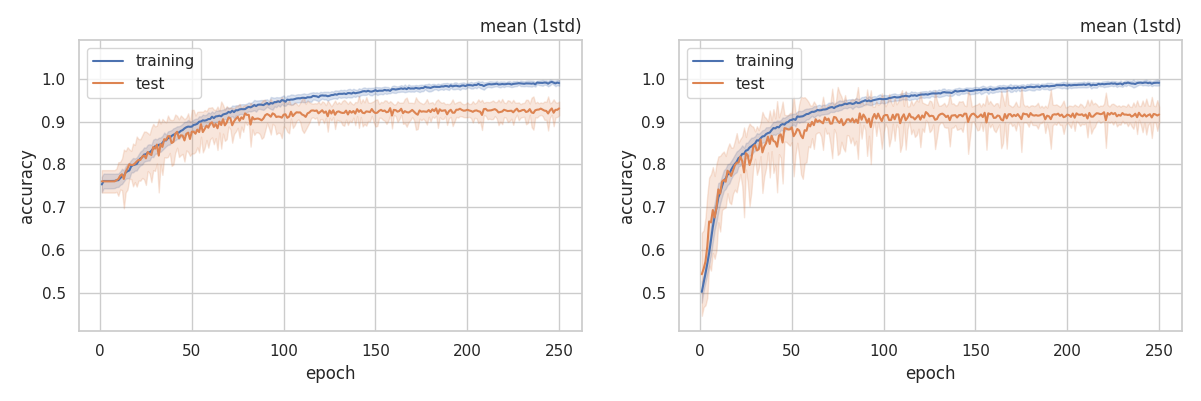
\includegraphics[width=1\hsize, keepaspectratio]{images/drawio/4_3_accs.png}
  \caption{accuracyの学習遷移\\(左 : インバランスドデータ 右 : バランスドデータ)}
  \label{fig:4_3_accs}
\end{figure}
 
\begin{figure}[H]
  \centering
  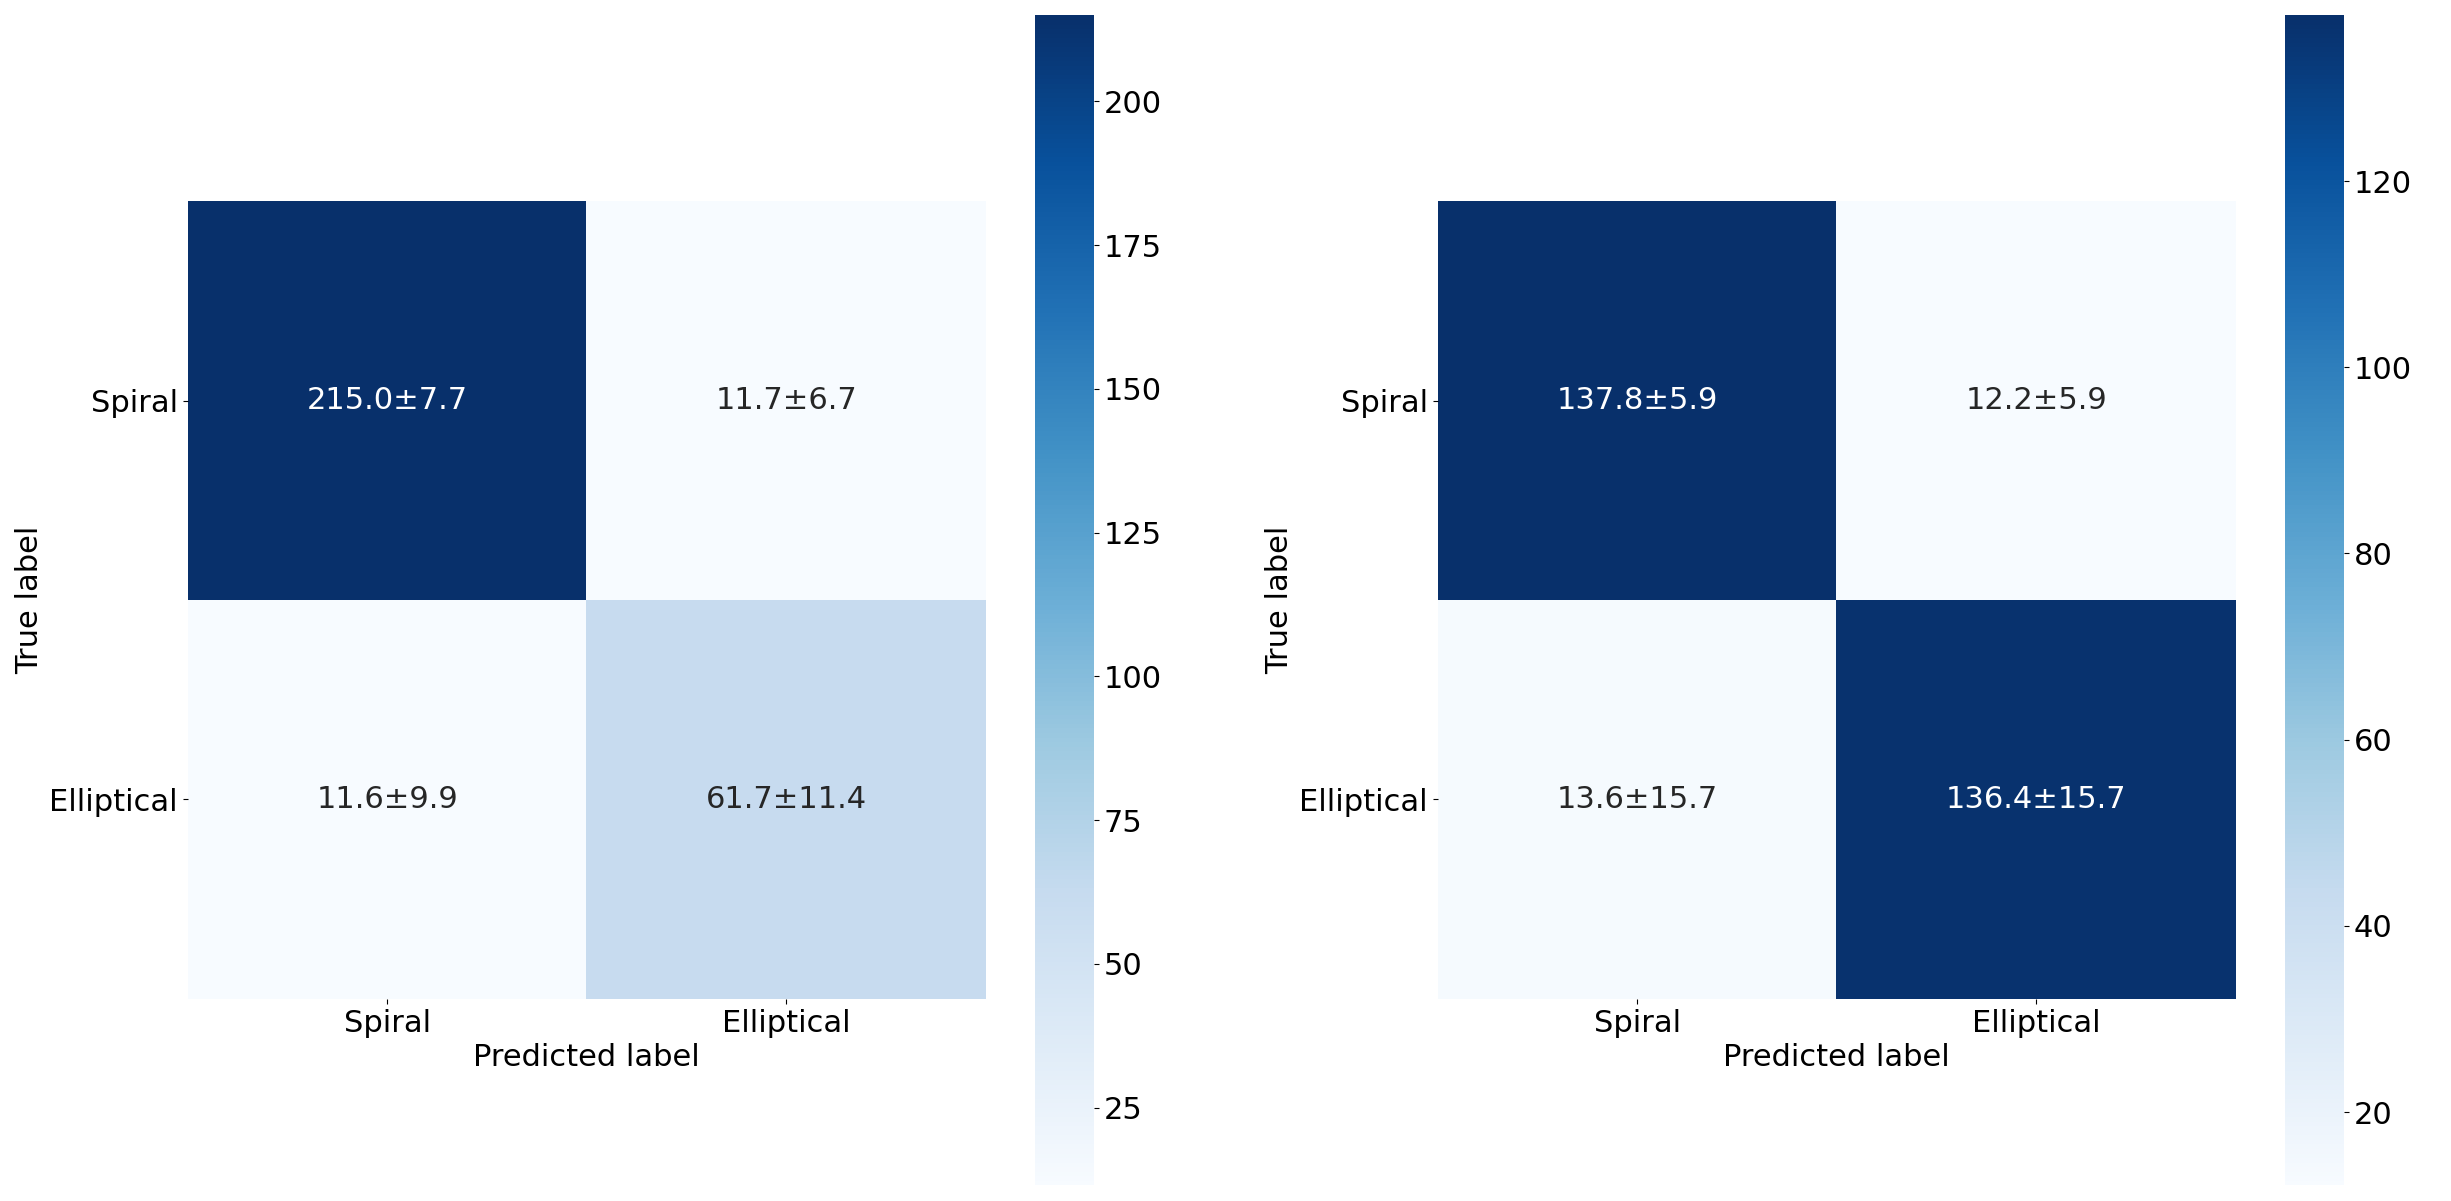
\includegraphics[width=1\hsize, keepaspectratio]{images/drawio/4_3_cms.png}
  \caption{混同行列\\(左 : インバランスドデータ 右 : バランスドデータ)}
  \label{fig:4_3_cms}
\end{figure}


% \subsubsection{モデル学習の進行}
% 図\ref{fig:losses_ex4-2-2}・図\ref{fig:accs_ex4-2-2}において,テストデータに対するスコアが100epoch付近までloss関数は降下,accuracyは上昇するものの,それ以降のepochではloss関数は上昇するがaccuracyは横ばいになっている.このことから,インバランスドデータで学習を行ったモデルは100epoch目以降学習データに対し過適合はしているものの,テストデータに対する汎化性能は失っていないことが読み取れる.

% また図\ref{fig:losses_ex4-3}・図\ref{fig:accs_ex4-3}において,テストデータに対するスコアが75epoch付近までloss関数は降下,accuracyは上昇するものの,それ以降のepochではloss関数は上昇するがaccuracyは横ばいになっている.このことから,バランスドデータで学習を行ったモデルは75epoch目以降学習データに対し過適合はしているものの,テストデータに対する汎化性能は失っていないことが読み取れる.

\subsubsection{テストデータに対するaccuracyの評価}
モデルの形態分類性能を評価するため,両モデル間にてテストデータに対する予測のaccuracyの比較を行う.性能評価においては,4.2節同様,モデルが学習しきった際の分類性能を用いた.

両モデルにおける,テストデータへの予測精度(accuracy)を表\ref{tb:accs_4.3}に示す.表\ref{tb:accs_4.3}は4.2節における表\ref{tb:accs_4.2}と同様の形式であり,今回の30回実行におけるaccuracyの平均値と標準偏差をそれぞれ1$\sigma$分記載した.表\ref{tb:accs_4.3}より,テストデータに対する予測のaccuracyの標準偏差付き平均値において両モデル間で有意な差はなかった.

\subsubsection{TSSの導出方法,および両分類モデルの分類性能評価}
次に,データセット内のクラスインバランスに左右されづらい評価指標であるTSSにて,再度両モデルの評価・性能比較を行う.

% TSSを導出するため,先ほど求めた「モデルが学習しきった地点と思われる,テストデータに対するaccuracyが最大となるepoch数」まで,再度30回学習およびテストを両モデルにて行った.今回行ったこの再度30回学習およびテストをした結果は,後ほど混同行列の導出にも用いる.

両モデルのテストデータへの予測精度(TSS)を表\ref{tb:TSS_4.3}に示す.
表\ref{tb:TSS_4.3}より,標準偏差付き平均値を見たとき,TSSが両モデルとも0.8付近と高いスコアを記録しており,また両モデルにおける有意差はなかった.
TSSは両クラスの分類性能がどちらも高くないと数値が向上しない評価指標のため,
両モデルとも片方のクラスについて分類する性能が高いモデルではなく,両クラスへの分類性能をもつ分類モデルであることが分かる.

\subsubsection{混同行列によるモデルの評価}
最後に,混同行列を用いて各モデルのテストデータに対する予測精度の比較を行う.

図\ref{fig:4_3_cms}より,インバランスドデータを用いて学習およびテストを行ったモデルにおいて陽性を渦巻銀河とした場合のtrue positive rateは$215.0/(215.0+11.7) = 0.948$,楕円銀河とした場合は$61.7/(11.6+61.7) = 0.842$であることが分かる.
同様に図\ref{fig:4_3_cms}より,バランスドデータを用いて学習およびテストを行ったモデルにおいて陽性を渦巻銀河とした場合のtrue positive rateは$137.8/(137.8+12.2) = 0.919$,楕円銀河とした場合は$136.4/(13.6+136.4) = 0.909$であることが分かる.
2つのモデルを比較すると,インバランスドデータモデルは楕円銀河のtrue positive rateが0.9以下であるのに対し,バランスドデータは両クラスのtrue positive rateが0.9以上であることが分かる.このことから,インバランスドデータモデルは渦巻銀河のデータ数が多い分,渦巻銀河を渦巻銀河と分類する能力が高く,またバランスドデータモデルは渦巻銀河を渦巻銀河と,楕円銀河を楕円銀河と分類する能力が同程度に高いモデルであることが分かる.

% \begin{table}[htbp]
%   \centering
% 	\caption{インバランスドデータで学習を行ったモデル,およびバランスドデータで学習を行ったモデルのテストデータに対する予測のaccuracy}
%   \begin{tabular}{|c|c|c|}
% 		\hline
%     & mean$\pm$std (2$\sigma$) & mean$\pm$ste (2$\sigma$) \\ \hline
%     インバランスドデータでのモデル & $0.931 \pm 0.034$(158th epoch) & $0.931 \pm 0.006$(158th epoch) \\ \hline
%     バランスドデータでのモデル & $0.922 \pm 0.036$(123th epoch) & $0.922 \pm 0.007$(123th epoch) \\ \hline
%   \end{tabular}
%   \label{tb:accs_4.3}
% \end{table}

\begin{table}[H]
  \centering
	\caption{ラベルインバランスによるaccuracyの変化}
  \begin{tabular}{|c|c|}
		\hline
    & mean (1std) \\ \hline
    インバランスドデータでのモデル & $0.931 \pm 0.017$(158th epoch) \\ \hline
    バランスドデータでのモデル & $0.922 \pm 0.018$(123th epoch) \\ \hline
  \end{tabular}
  \label{tb:accs_4.3}
\end{table}

% \begin{table}[htbp]
%   \centering
% 	\caption{インバランスドデータで学習を行ったモデル,およびバランスドデータで学習を行ったモデルのテストデータに対する予測のTSS}
%   \begin{tabular}{|c|c|c|}
% 		\hline
%     & mean$\pm$std (2$\sigma$) & mean$\pm$ste (2$\sigma$) \\ \hline
%     インバランスドデータでのモデル & $0.791 \pm 0.250$ & $0.791 \pm 0.046$ \\ \hline
%     バランスドデータでのモデル & $0.828 \pm 0.184$ & $0.828 \pm 0.033$ \\ \hline
%   \end{tabular}
%   \label{tb:TSS_4.3}
% \end{table}

\begin{table}[H]
  \centering
	\caption{ラベルインバランスによるTSSの変化}
  \begin{tabular}{|c|c|}
		\hline
    & mean (1std) \\ \hline
    インバランスドデータでのモデル & $0.791 \pm 0.125$ \\ \hline
    バランスドデータでのモデル & $0.828 \pm 0.092$ \\ \hline
  \end{tabular}
  \label{tb:TSS_4.3}
\end{table}

\newpage
\section{議論}
4.2節では,不確かな天体とラベル付けされている天体をモデル学習およびテストに用いた際の分類精度への影響を調べるため,不確かな天体を使用したモデルと除外したモデルを作成し,両モデルの比較を行った.
その結果,4.2節の実験にて不確かな天体を入れた3値分類問題とした方がテストデータに対する予測精度が落ちてしまう現象が確認された.
この現象には2つの可能性が考えられる.1つ目は,GZの形態分類フラグで不確かな天体と判定された天体が実際は渦巻銀河であったり楕円銀河である可能性である.GZの形態分類フラグは,渦巻銀河および楕円銀河の投票率が0.8である場合に渦巻および楕円というフラグが立ち,それ以外の場合は不確かな天体にフラグが立つ.渦巻および楕円と不確かな天体は0.8という閾値で区切られているが,この閾値では渦巻銀河および楕円銀河が不確かな天体とフラグ付けされている可能性がある.このようにクラスのラベル付けが間違っているデータをモデルに用いた場合,モデルの学習は問題なく進むが,テストデータへの分類精度は低下する.
2つ目は,GZの形態分類フラグにて星もしくは分からない天体とマージャーが全て不確かな天体と判定されるため,不確かな天体クラスの天体種類に多様性が存在する可能性である.GZの形態分類フラグでは,星もしくは分からない天体とマージャーの投票率が最も高い天体には不確かな天体と判定されている.このため,不確かな天体クラスは実際には,人間による判定の信頼度が低い(すなわち0.8の投票率に届かなかった)渦巻銀河および楕円銀河・星もしくは分からない天体・マージャーの4つが混在していると考えられる.この不確かな天体クラス内の天体種類の多様性が,モデルの不確かな天体についての学習を難しくしており,結果としてテストデータに対する予測精度が低下する可能性がある.


4.3節では,使用する天体の銀河形態ラベルのクラスインバランスがモデルの分類精度に与える影響を調べるため,渦巻銀河と楕円銀河の比率が異なるインバランスデータを用いたモデルと,比率を等しくしたバランスドデータを用いたモデルを作成し,両モデルの比較を行った.
その結果,4.3節の実験にて学習・テストに用いるデータ内のクラスインバランス改善を行っても分類精度の改善が見受けられなかった.このことから,今回の実験で見受けられたようなクラスインバランスでは,分類精度への影響は小さい可能性がある.もしデータセット内に桁数が異なるほどのクラスインバランスが起きていた場合,インバランスを改善せずにモデル作成を行った場合,分類精度に悪影響が発生する可能性がある.
% もし学習データ内にて桁数が異なるほどの強いデータインバランスが起きていた場合,データインバランス改善を行えば分類精度が改善される可能性がある.

4章の目標は学習データとテストデータの解像度が揃っているという条件のもと,どの程度の精度の分類モデルを作成することができるかを確認することであり,そのために2つの実験を行った.GZにて不確かと分類されている天体を除外し,渦巻銀河・楕円銀河の2値分類問題とすることで,分類モデルの分類精度は大きく向上した.一方で,学習・テストに用いるデータ内のデータインバランスを改善しても分類精度に有意差が認められるほどの向上は見受けられなかった.本論文における今後の実験では,渦巻銀河を分類することに特化したモデルでなく,渦巻銀河・楕円銀河の両者を分類することを優先するため,渦巻銀河・楕円銀河のtrue positive rateがある程度等しくなることが見込めるバランスドデータにてモデル学習を行っていく.具体的には,モデルの学習およびテストに用いる天体数はクラスごとに等しくなるようにし,また学習データおよびテストデータのクラスの比率が等しくなるようにデータ分けを行うものとする.



\newpage
\chapter{空間解像度差のあるデータセットを用いた分類モデル作成}
% 本研究の将来展望は,高空間分解能観測装置データを用いてモデル学習を行うことで,既存の低空間分解能データセットに対し更なる高精度形態分類を提供するというものである.この将来展望の前提条件である,学習データとテストデータとの間の解像度が揃っているデータセットにて高精度の銀河形態分類モデルを学習させることを,第4章にて達成することができた.

% そこで,
この章では
% 将来展望で行われる予定の
異なる観測装置データの組み合わせを念頭に置き,学習データとテストデータとの間に解像度差があるデータセットにて形態分類モデルの作成が行えるかを検証する.

\section{実験概要}
第5章ではSDSSから取得した銀河切り出し画像とGZから取得した分類フラグを学習データとしてモデルを学習させ,銀河切り出し画像を縮小した低解像度データセットに対し予測を行う.なお,学習・テストに用いる天体データの銀河種は渦巻銀河・楕円銀河の2つとする.

\subsubsection{学習データ}
学習データには第4章で用いた14,998天体のうち不確かな天体を除いた,渦巻銀河4,057天体,楕円銀河1,561天体の計5,618天体を用いた.

\subsubsection{縮小画像データセット(テストデータ)の作成方法}
この章ではテストデータとして,SDSSから取得した銀河切り出し画像を縮小したデータセットを使用する.学習データにも用いている5,618天体を,平均画素法により縮小処理を施した.平均画素法とは画像処理法の一つであり,縮小前画像と縮小画像の画像サイズの面積比を用いて,画像の縮小を行う方法である.画像の縮小にはOpenCVに実装されているresize関数のINTER\_AREAメソッドを使用した.ここでresize関数は画像の拡大または縮小を行う関数であり,INTER\_AREAメソッドとは平均画素法による画像補間処理を行うメソッドである.
銀河切り出し画像を1/2, 1/3, ..., 1/7, 1/8倍に縮小し,計7つの縮小画像データセットを作成した.縮小画像の例として,1/4倍に縮小した画像群を図\ref{fig:shrink_1_4}に示す.

\begin{figure}[H]
 \centering
 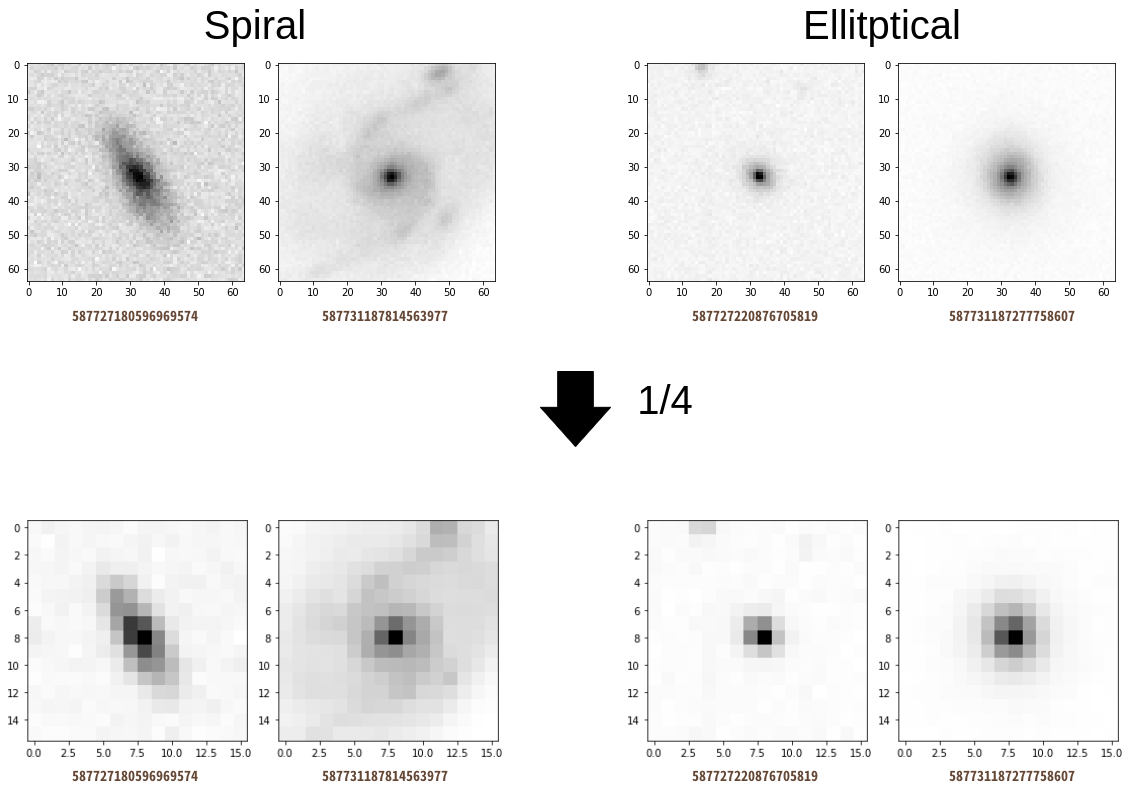
\includegraphics[width=13cm]{images/5syou/syuron_5syou_kakudai/ver1/5syou_shrink_ver1.png}
 \caption{銀河切り出し画像の縮小例(1/4倍)}
 \label{fig:shrink_1_4}
\end{figure}

\subsubsection{縮小画像データセットの拡大方法}
モデルに画像データを入力する際,用いる画像サイズは揃えて入力する必要があり,今回の実験条件では学習データである高解像度データの画像サイズへ揃える必要がある.
そのため,今回の実験ではテストデータである縮小画像データセットを拡大してモデルに入力する.

縮小画像の拡大には,OpenCVのresize関数を用いた.この章での実験において,画像拡大の際の補間方法として最近傍補間,バイリニア補間,バイキュービック補間を使用した.画像拡大の例として,1/4倍に縮小された銀河切り出し画像の,各補間方法による画像拡大の例を図\ref{fig:kakudai_1_4}に示す.なお図\ref{fig:kakudai_1_4}にて用いられている縮小画像は,図\ref{fig:shrink_1_4}のものと同様である.

\begin{figure}[H]
 \centering
 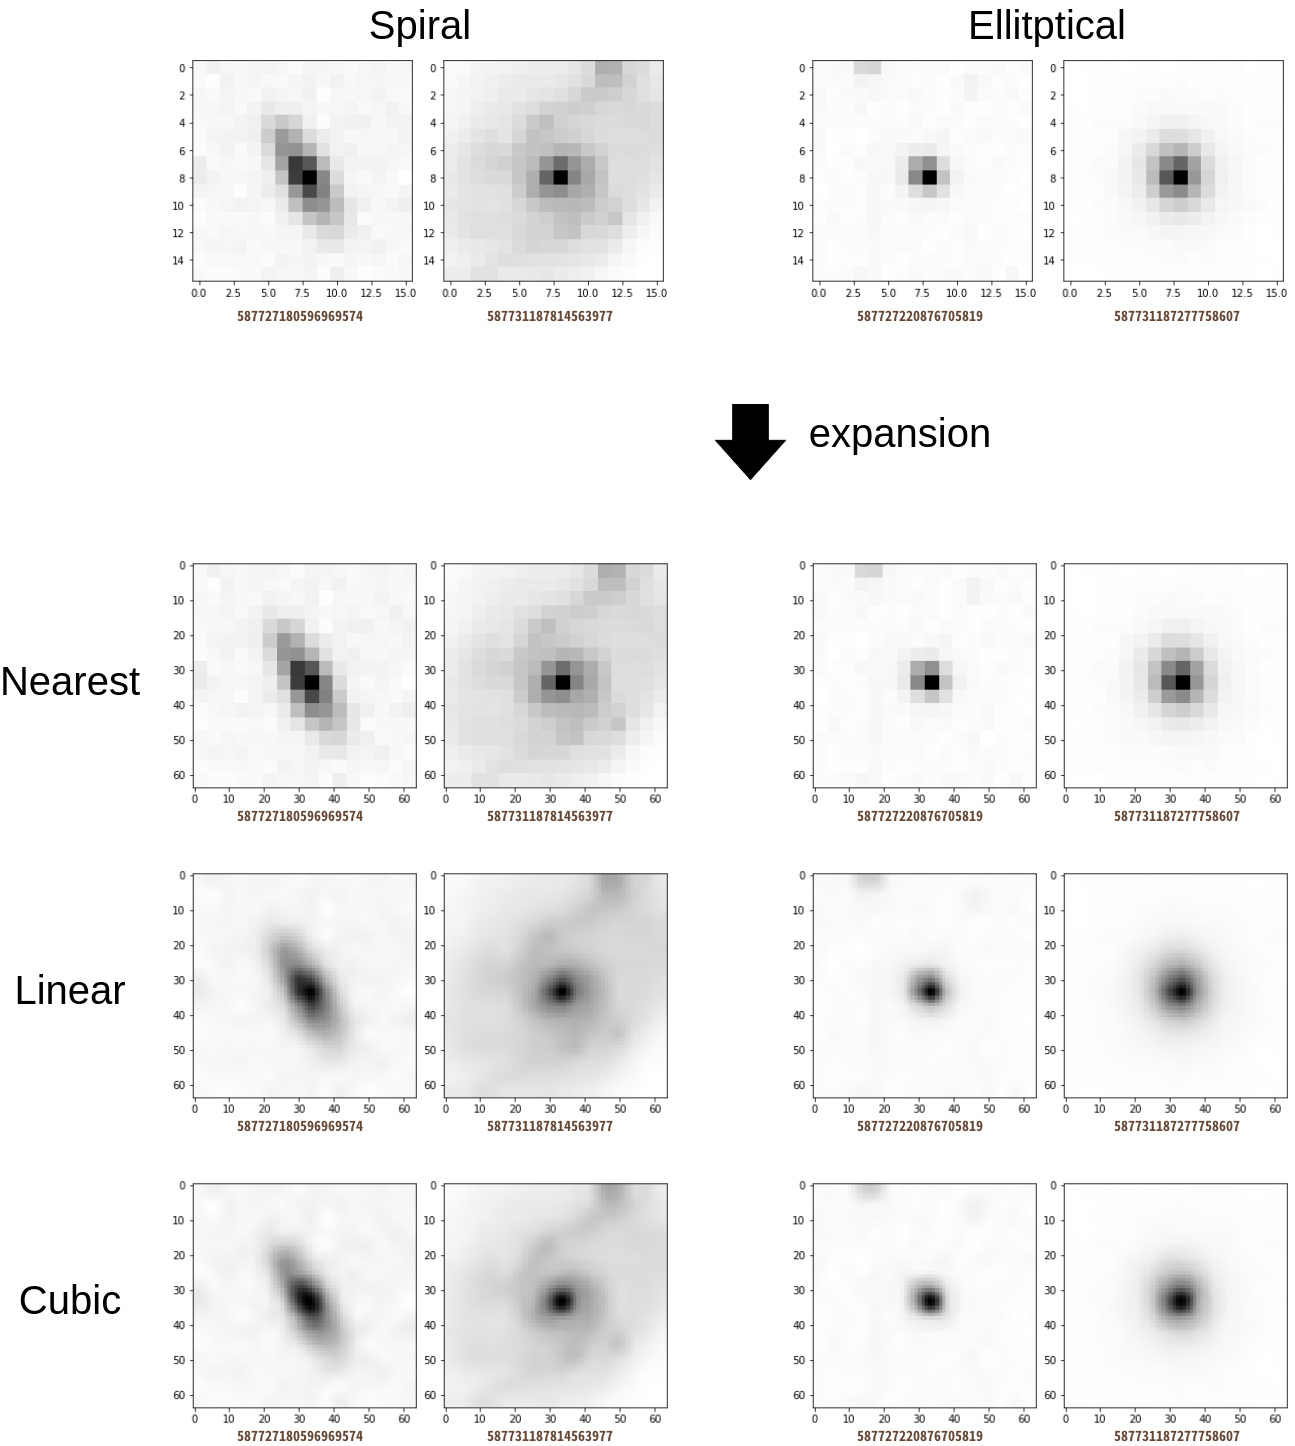
\includegraphics[width=13cm]{images/drawio/5syou_kakudai.png}
 \caption{1/4倍縮小画像の画像拡大例\\(最近傍補間・バイリニア補間・バイキュービック補間)}
 \label{fig:kakudai_1_4}
\end{figure}

\subsubsection{モデル構造}
第5章で学習させる深層学習モデルは,第4章と同じ構造のものを使用した.
 
\subsubsection{モデルの評価方法}
モデルの評価指標はaccuracy(正解率)を使用した.


\section{分類精度のデータセット内解像度差依存性}
この節では,学習データとテストデータとの間に解像度差がある状況において,テストデータへの予測が成立するか,また予測が成立する場合には解像度差がいくつまでならば使用可能かについて検証を行った.このうち「使用可能」の定義としては,学習データとテストデータの解像度が揃っている状況での予測結果である''Original''と同程度のaccuracyであることとする.

\subsection{実験条件}
使用する天体は4.3節での実験と同様に,不確か天体を除いた5,618天体を母集団とした.本研究の将来展望にて,モデル学習に使う天体数は少数であることが望ましいとしているため,クラスごとの使用天体数は第4章で行った実験よりも少ない300天体とした.モデルの学習データにはSDSSの切り出し画像,テストデータにはSDSSの切り出し画像を縮小した画像をそれぞれ用いた.

モデルの学習期間は900epochとした.これは,すべての縮小データの縮小倍率にて,モデルが十分に学習しきる期間,すなわちテストデータに対するaccuracyが減少傾向を見せるepochが900epochであったからである.

学習させたモデルは第4章と同様に30回の学習を行い,平均値および標準偏差を導出した.


\subsection{実験結果}
銀河切り出し画像を1/2, 1/3, ..., 1/8倍に縮小した縮小データに対する,形態分類モデルの予測結果を図\ref{fig:inter_comparison_300_1std}に示す.横軸がテストデータである縮小データの縮小倍率であり,縦軸がテストデータに対する予測のaccuracyとなっている.accuracyについては,30回実行における平均値と1標準偏差をエラーバー形式で示している.なお,図\ref{fig:inter_comparison_300_1std}の一番左に位置しているOriginalとなっている箇所は,テストデータに縮小データでなく,学習データと同じ大きさの銀河切り出し画像を使用してテストを行った結果である.すなわち,Originalが学習データとテストデータの解像度が揃っている状況での予測結果に対し,1/2から1/8が学習データとテストデータとの間に解像度差がある状況での予測結果となっている.凡例には,エラーバーの各色と拡大方法の対応付けが示されている.

また,各モデルの縮小データに対する予測精度を表\ref{tb:accs_4_2_nearest_1std}から表\ref{tb:accs_4_2_cubic_1std}に示す.表にはテストデータに対する分類精度が最大となるepochのaccuracyを掲載した.

% \begin{figure}[H]
%  \centering
%  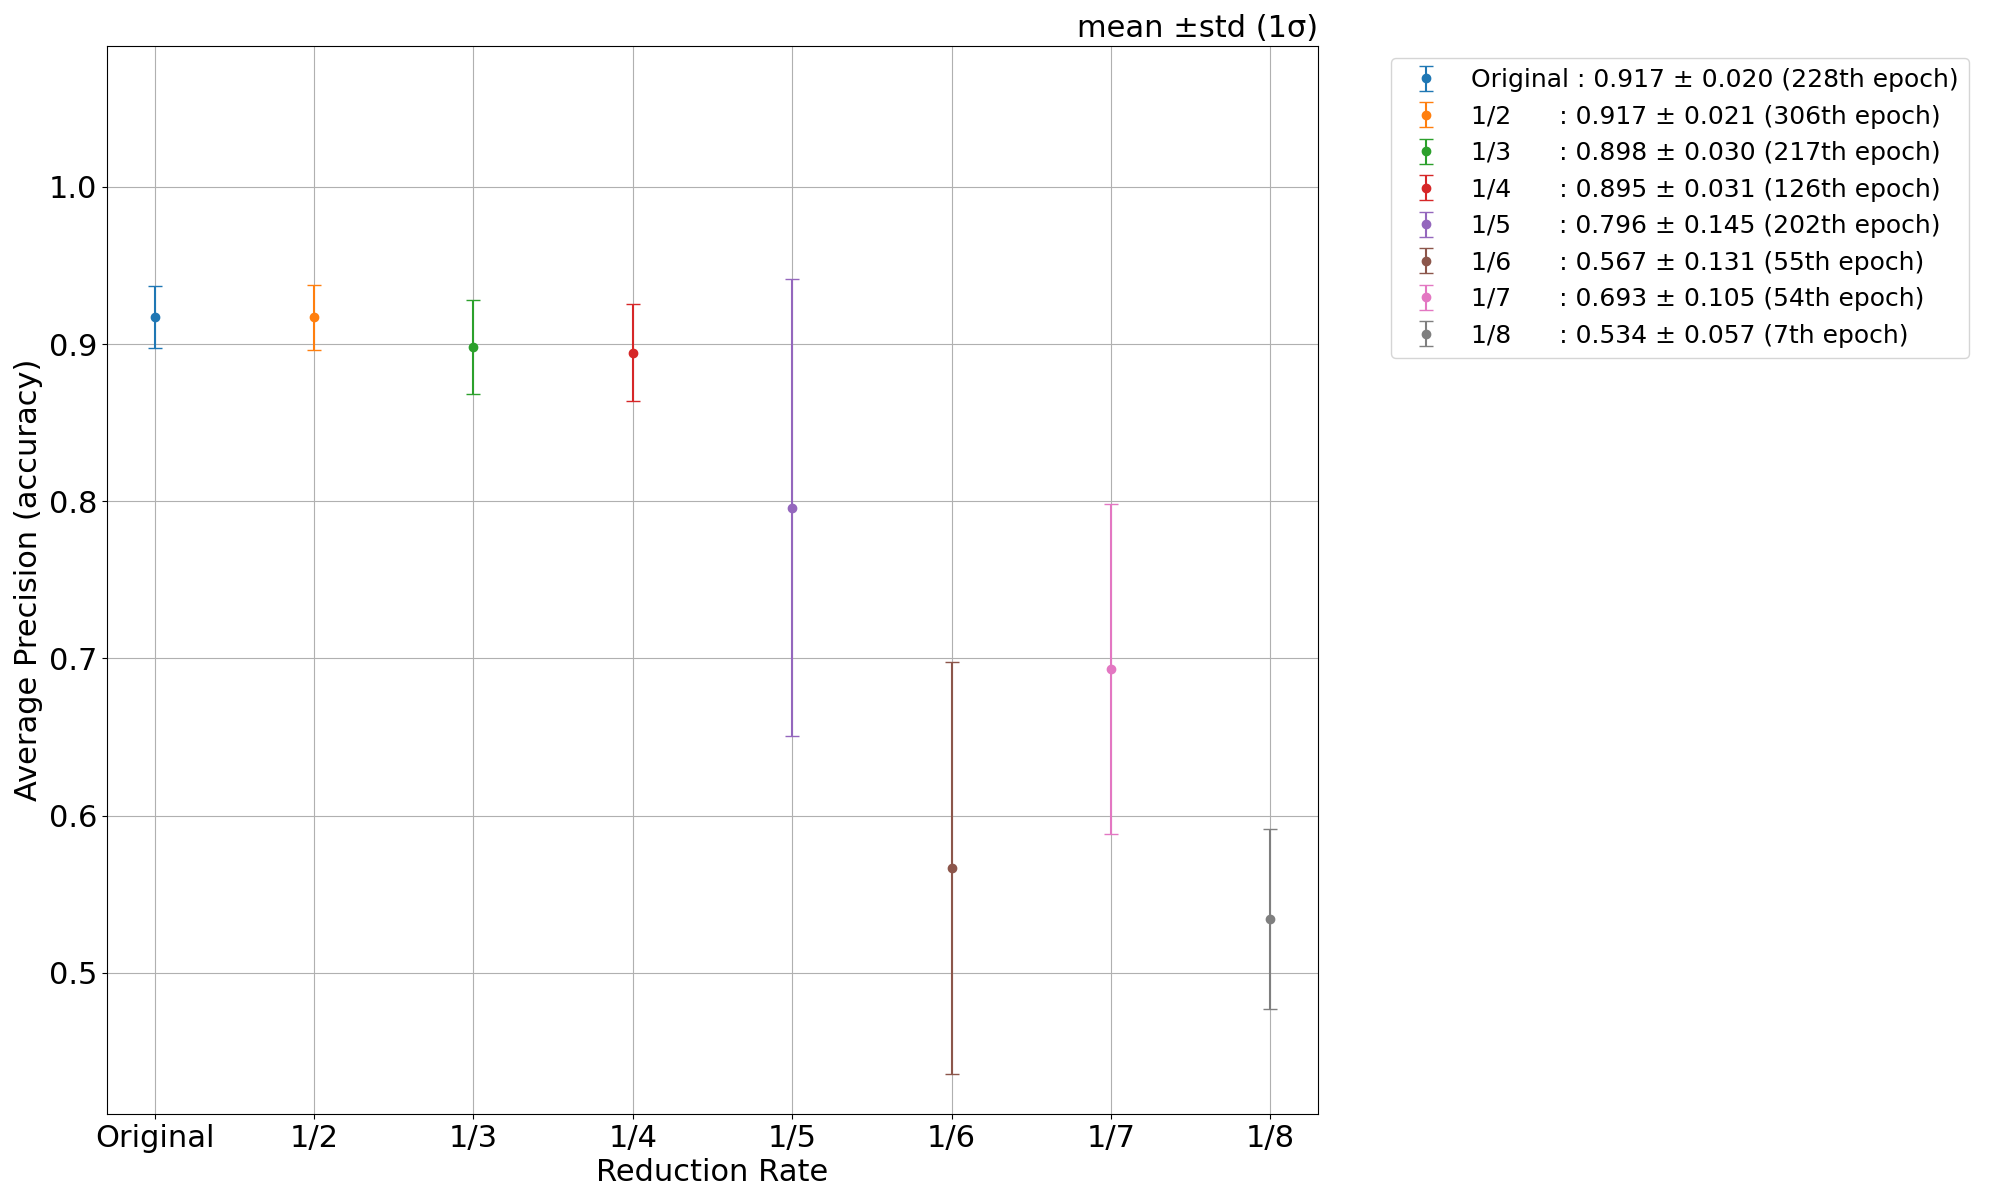
\includegraphics[width=16cm]{images/5syou/print_errorbar/nearest/acc_with_errorbar_syuron5_nearest_900epoch_30run_300_acc_max_std1sigma.png}
%  \caption{最近傍補間によって内挿された,縮小データに対するモデルの予測結果(1std)}
%  \label{fig:nearest_300_1std}
% \end{figure}

% \begin{figure}[H]
%   \centering
%   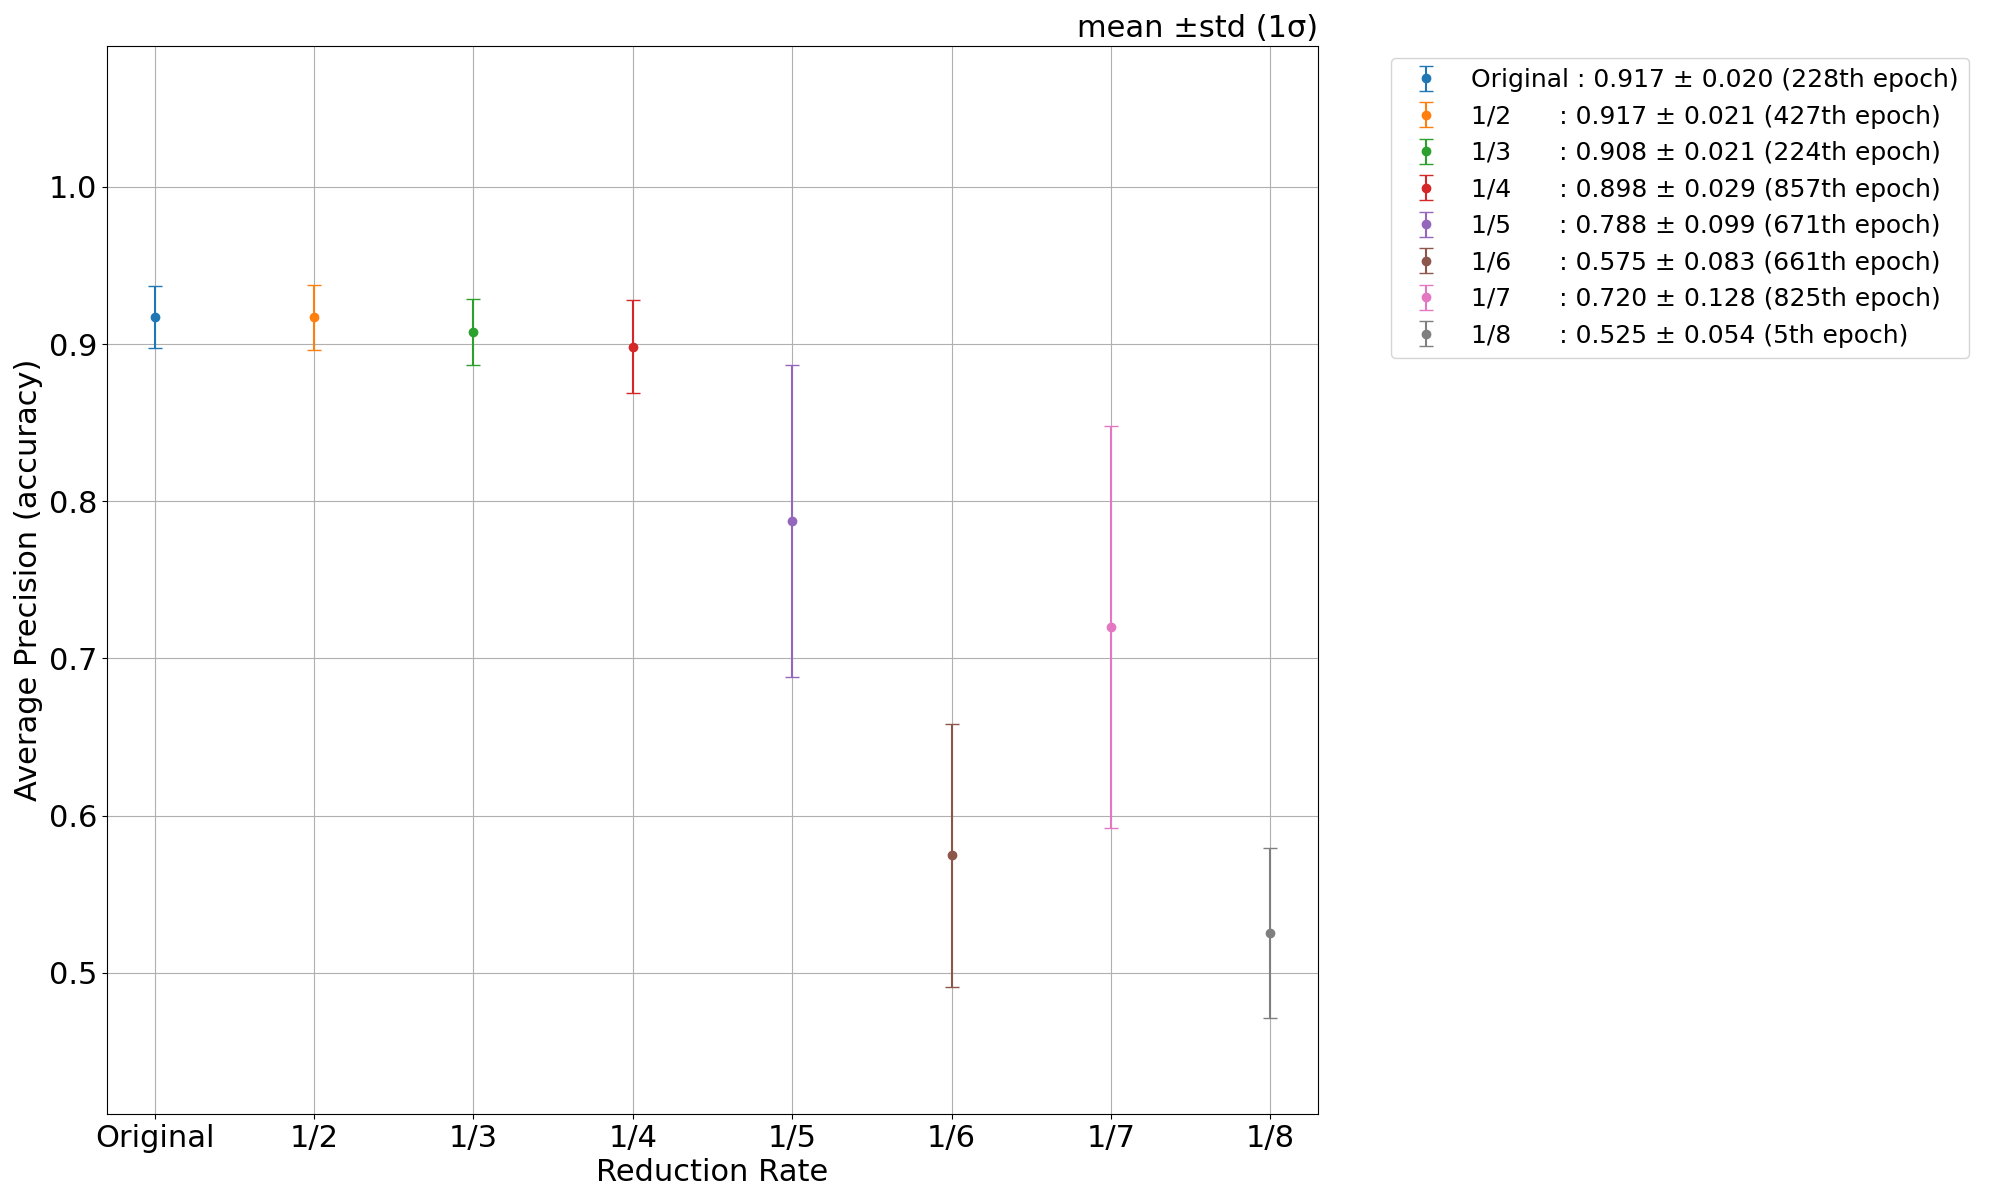
\includegraphics[width=16cm]{images/5syou/print_errorbar/linear/acc_with_errorbar_syuron5_linear_900epoch_30run_300_acc_max_std1sigma.png}
%   \caption{バイリニア補間によって内挿された,縮小データに対するモデルの予測結果(1std)}
%   \label{fig:linear_300_1std}
% \end{figure}

% \begin{figure}[H]
%   \centering
%   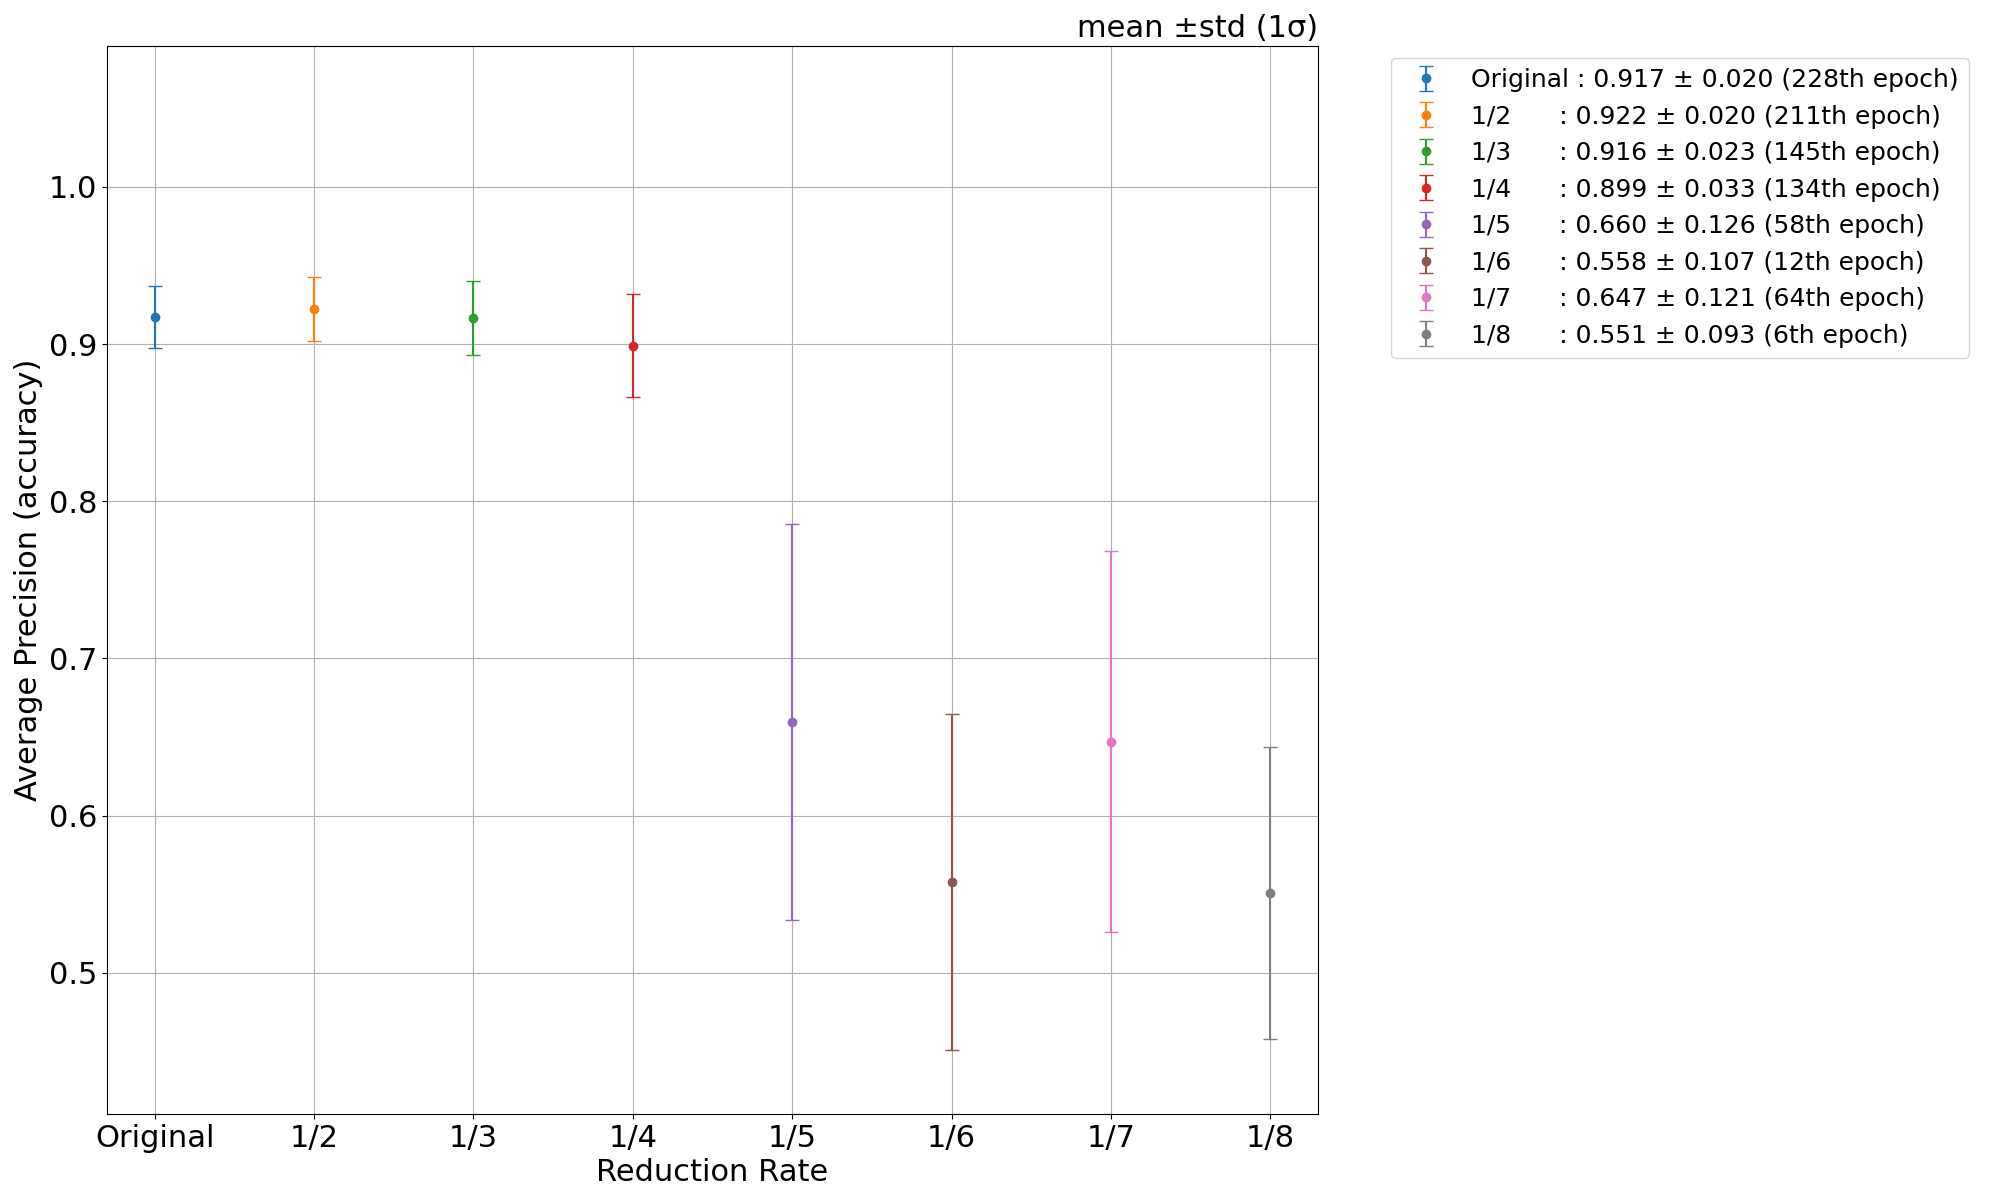
\includegraphics[width=16cm]{images/5syou/print_errorbar/cubic/acc_with_errorbar_syuron5_cubic_900epoch_30run_300_acc_max_std1sigma.png}
%   \caption{バイキュービック補間によって内挿された,縮小データに対するモデルの予測結果(1std)}
%   \label{fig:cubic_300_1std}
% \end{figure}

\begin{figure}[H]
  \centering
  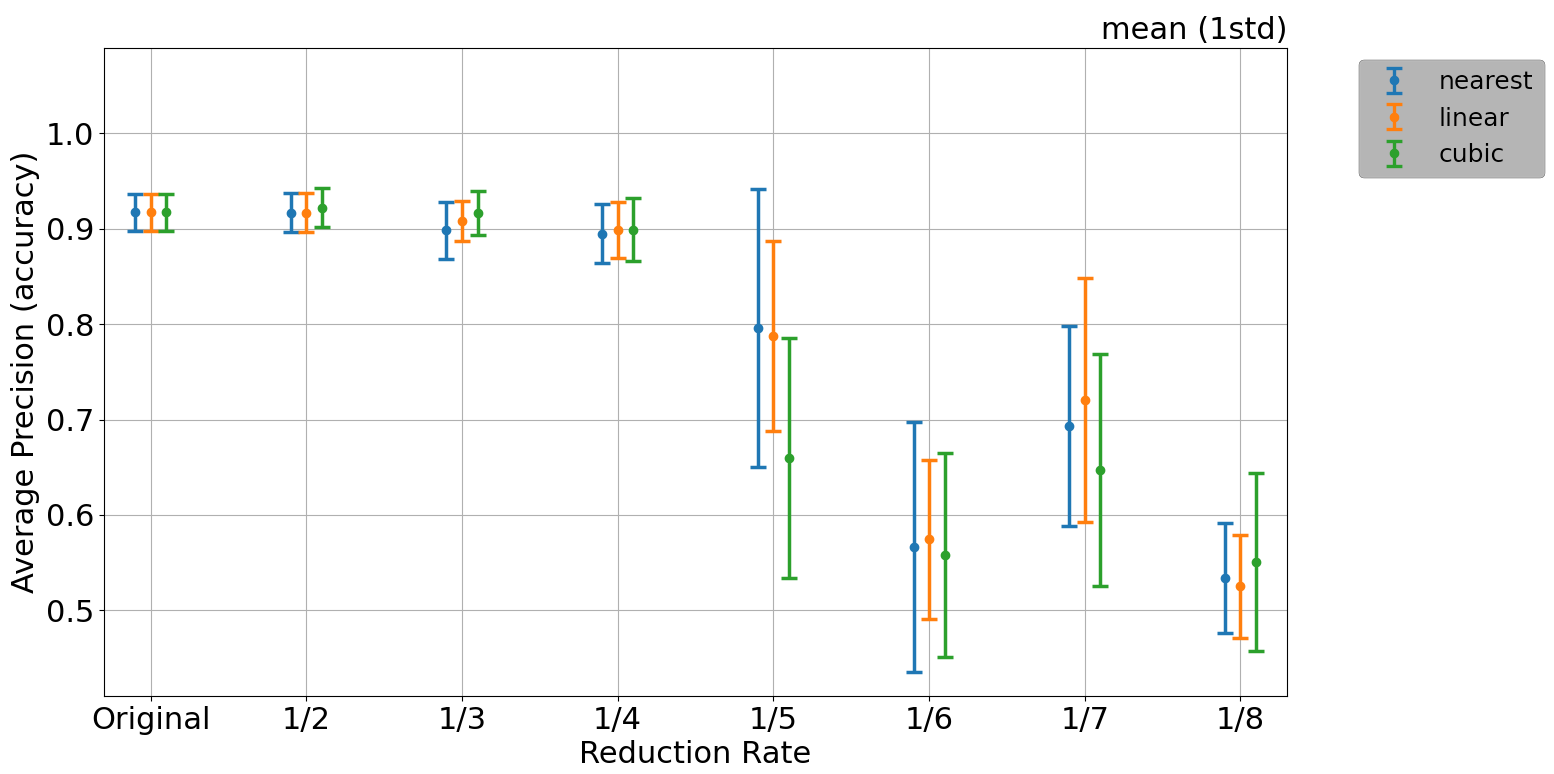
\includegraphics[width=1\hsize, keepaspectratio]{images/5syou/print_errorbar/print_errorbar_inter_comparison/acc_with_errorbar_syuron5_inter_comparison_900epoch_30run_300_acc_max_std1sigma.png}
  \caption{縮小データに対する予測精度(1標準偏差)}
  \label{fig:inter_comparison_300_1std}
\end{figure}

\begin{table}[H]
  \centering
	\caption{最近傍補間によって拡大したテストデータに対する予測精度(1標準偏差)}
  \begin{tabular}{|c|c|}
		\hline
    & mean (1std) \\ \hline
    Original & $0.917 \pm 0.020$(228th epoch) \\ \hline
    1/2 & $0.917 \pm 0.021$(306th epoch) \\ \hline
    1/3 & $0.898 \pm 0.030$(217th epoch) \\ \hline
    1/4 & $0.895 \pm 0.031$(126th epoch) \\ \hline
    1/5 & $0.796 \pm 0.145$(202th epoch) \\ \hline
    1/6 & $0.567 \pm 0.131$(55th epoch) \\ \hline
    1/7 & $0.693 \pm 0.105$(54th epoch) \\ \hline
    1/8 & $0.534 \pm 0.057$(7th epoch) \\ \hline
  \end{tabular}
  \label{tb:accs_4_2_nearest_1std}
\end{table}

\begin{table}[H]
  \centering
	\caption{バイリニア補間によって拡大したテストデータに対する予測精度(1標準偏差)}
  \begin{tabular}{|c|c|}
		\hline
    & mean (1std) \\ \hline
    Original & $0.917 \pm 0.020$(228th epoch) \\ \hline
    1/2 & $0.917 \pm 0.021$(427th epoch) \\ \hline
    1/3 & $0.908 \pm 0.021$(224th epoch) \\ \hline
    1/4 & $0.898 \pm 0.029$(857th epoch) \\ \hline
    1/5 & $0.788 \pm 0.099$(671th epoch) \\ \hline
    1/6 & $0.575 \pm 0.083$(661th epoch) \\ \hline
    1/7 & $0.720 \pm 0.128$(825th epoch) \\ \hline
    1/8 & $0.525 \pm 0.054$(5th epoch) \\ \hline
  \end{tabular}
  \label{tb:accs_4_2_linear_1std}
\end{table}

\begin{table}[H]
  \centering
	\caption{バイキュービック補間によって拡大したテストデータに対する予測精度(1標準偏差)}
  \begin{tabular}{|c|c|}
		\hline
    & mean (1std) \\ \hline
    Original & $0.917 \pm 0.020$(228th epoch) \\ \hline
    1/2 & $0.922 \pm 0.020$(211th epoch) \\ \hline
    1/3 & $0.916 \pm 0.023$(145th epoch) \\ \hline
    1/4 & $0.899 \pm 0.033$(134th epoch) \\ \hline
    1/5 & $0.660 \pm 0.126$(58th epoch) \\ \hline
    1/6 & $0.558 \pm 0.107$(12th epoch) \\ \hline
    1/7 & $0.647 \pm 0.121$(64th epoch) \\ \hline
    1/8 & $0.551 \pm 0.093$(6th epoch) \\ \hline
  \end{tabular}
  \label{tb:accs_4_2_cubic_1std}
\end{table}

\subsubsection{縮小データの縮小倍率における結果}
図\ref{fig:inter_comparison_300_1std}より,Originalの結果(学習データとテストデータの解像度が揃っている状況での予測結果)と同程度のaccuracyを記録しているテストデータの縮小倍率が存在することが分かる.

各拡大方法に注目すると,最近傍補間によって拡大したテストデータに対する予測は,縮小倍率が1/2から1/4倍の縮小データに対しては使用可能であることが分かる.なお,縮小倍率が1/5倍の縮小データに対する予測においては,モデルの学習にかなりの上振れが起こらないと達成できないスコアであることから,使用可能ではないとの判断を行った.

同様に,バイリニア補間によって拡大したテストデータに対する予測は,縮小倍率が1/2から1/4倍の縮小データに対しては使用可能であり,またバイキュービック補間によって拡大したテストデータに対する予測は,縮小倍率が1/2から1/4倍の縮小データに対しては使用可能であった.

このことから,内挿方法によらず,学習データとテストデータの解像度差が1/4倍までであったら,テストデータとして使用可能であることが分かった.

\subsubsection{内挿方法間での比較}
内挿方法の間で,テストデータに対するaccuracyの細かい挙動を比較する.図\ref{fig:inter_comparison_300_1std}より,1/2から1/4倍,および1/6から1/8倍の縮小データにおいては,1標準偏差の誤差区間において内挿方法による有意差は見受けられない.また,1/5倍の縮小倍率においてはバイキュービック補間によって内挿したテストデータに対する予測のaccuracyが他2手法より劣って見えるが,1標準偏差の誤差区間においては他2手法との有意差は見られない.このことから,テストデータへの予測のaccuracyにおいて,テストデータの内挿方法における有意差はないことが分かった.

\subsubsection{標準誤差における予測結果}
図\ref{fig:inter_comparison_300_1std}では,1標準偏差を示した.
ここで,accuracyの標準偏差は30個のモデルがもつaccuracyの値のばらつきであり,またこのばらつきはモデルパラメータの初期値および毎回シャッフルされる使用天体によってもたらされるものである.この小節ではaccuracyのばらつきを除外するため,標準偏差から標準誤差を推定した.
1標準誤差をエラーバーで示した縮小データに対するaccuracyを図\ref{fig:inter_comparison_300_1ste}に示す.また,拡大方法別の1標準誤差の値を表\ref{tb:accs_4_2_nearest_1ste}から表\ref{tb:accs_4_2_cubic_1ste}に示す.

図\ref{fig:inter_comparison_300_1std}と図\ref{fig:inter_comparison_300_1ste}を比較すると,1標準誤差の誤差区間では各縮小倍率間で有意差が生じる.
例として,最近傍補間にて拡大を行ったデータに対する予測結果で,1標準偏差の誤差区間では縮小倍率1/2倍に対するaccuracyは$0.896 \sim 0.938$で縮小倍率1/3倍は$0.868 \sim 0.928$となり有意差はない.しかし,1標準誤差の誤差区間では縮小倍率1/2倍は$0.913 \sim 0.921$で縮小倍率1/3倍は$0.893 \sim 0.903$となり有意差が生じていることが読み取れる.
標準偏差の誤差区間では有意差が見られない場合に標準誤差の誤差区間では有意差が見受けられる場合があることから,本研究における深層学習モデルはモデルパラメータの初期値と毎回シャッフルされる使用天体の2つの要素による学習のばらつきがある程度大きく存在することが分かる.

また図\ref{fig:inter_comparison_300_1ste}より,誤差区間を1標準誤差とした場合に縮小倍率1/6倍と1/7倍に対する予測のaccuracyを比較すると,どの拡大方法においても結果に有意差が生じ,また1/6倍に対する予測結果よりも1/7倍の方が高いことが伺える.図\ref{fig:inter_comparison_300_1std}と図\ref{fig:inter_comparison_300_1ste}での傾向として,学習データとテストデータの解像度差が大きいほど,テストデータに対するaccuracyが減少することが見て取れるが,1/6倍に対する予測結果よりも1/7倍のほうが高い傾向は,これに反している.

\begin{figure}[H]
  \centering
  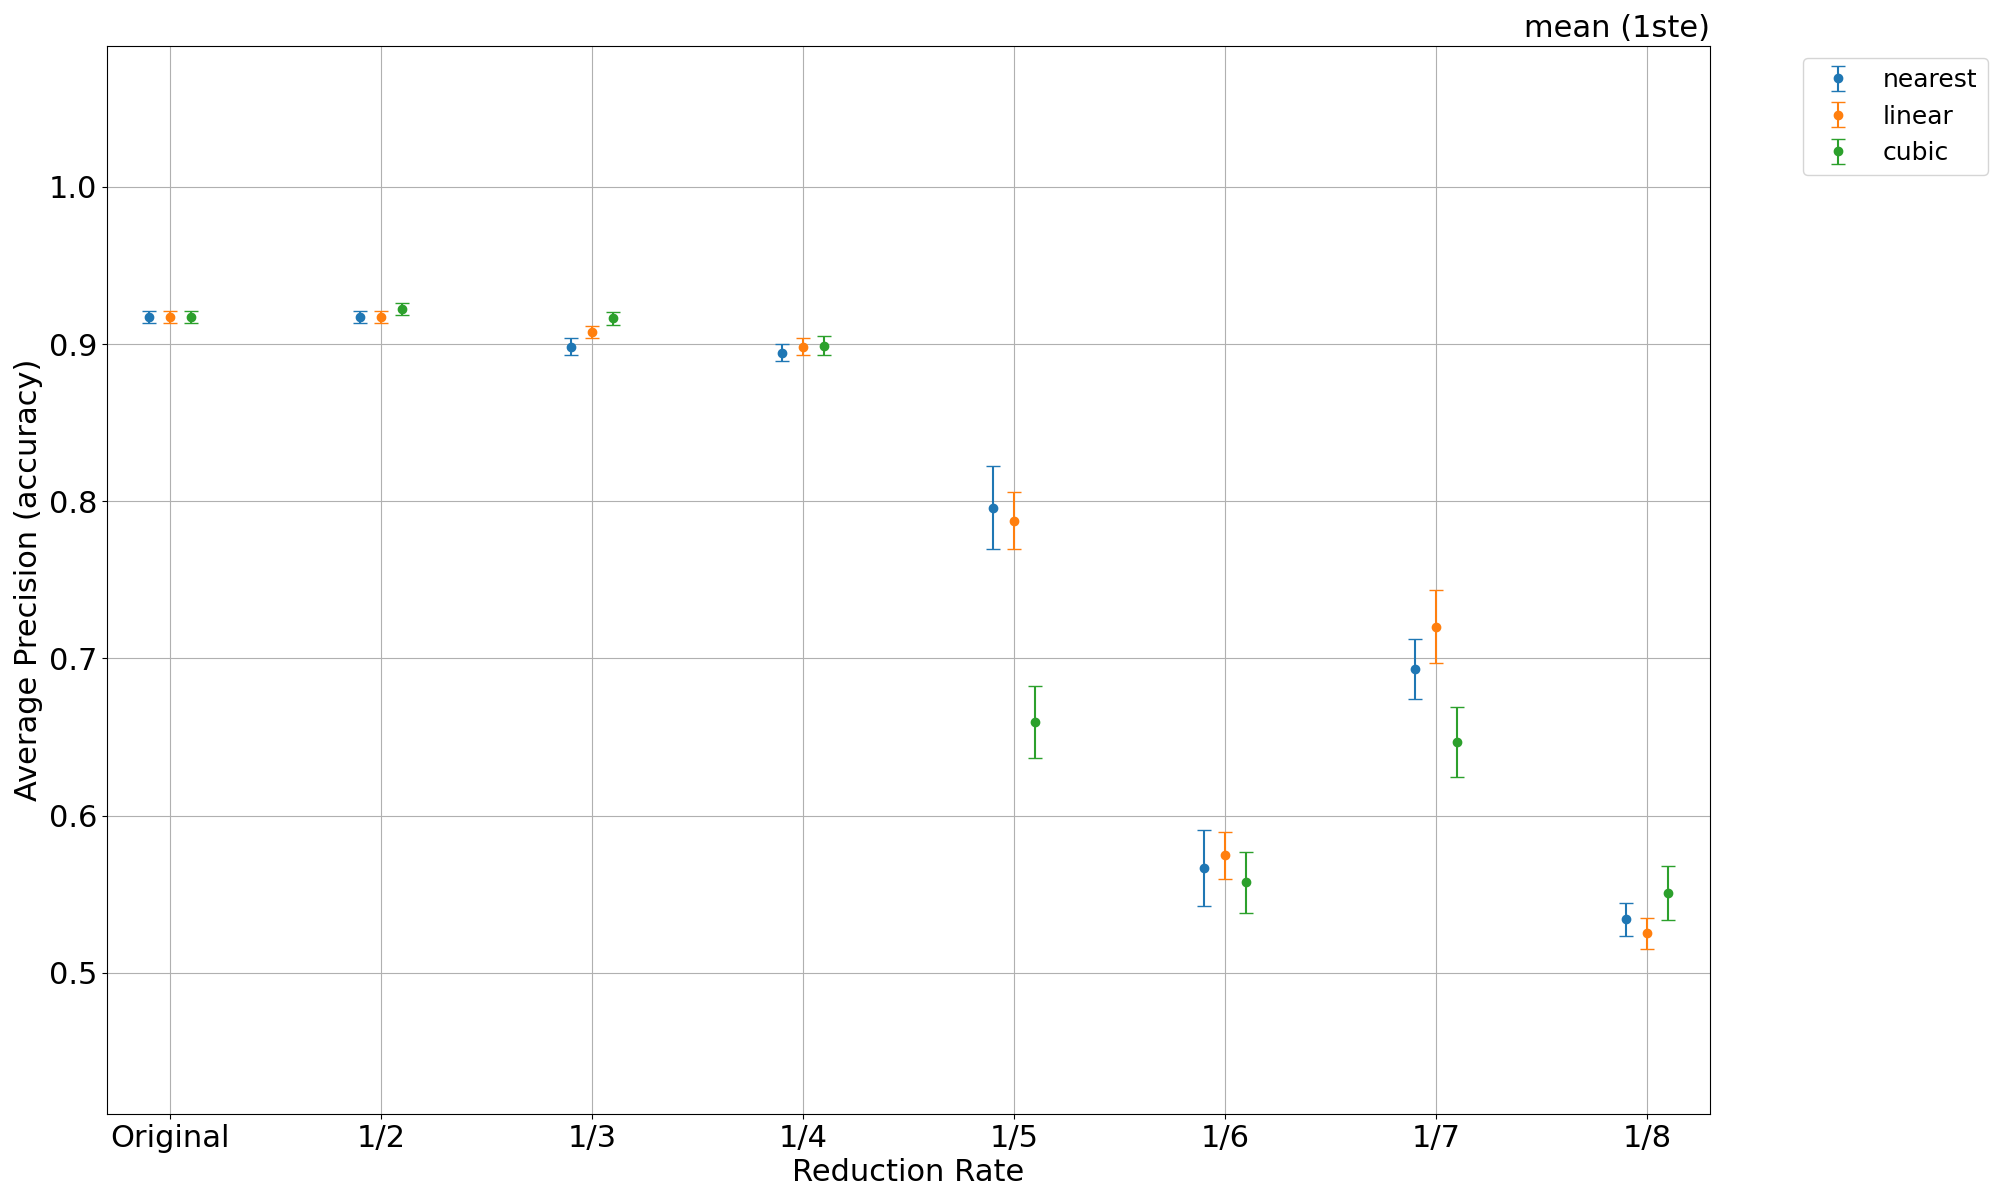
\includegraphics[width=16cm]{images/5syou/print_errorbar/print_errorbar_inter_comparison/acc_with_errorbar_syuron5_inter_comparison_900epoch_30run_300_acc_max_ste1sigma.png}
  \caption{縮小データに対する予測精度(1標準誤差)}
  \label{fig:inter_comparison_300_1ste}
\end{figure}

% \begin{figure}[H]
%   \centering
%   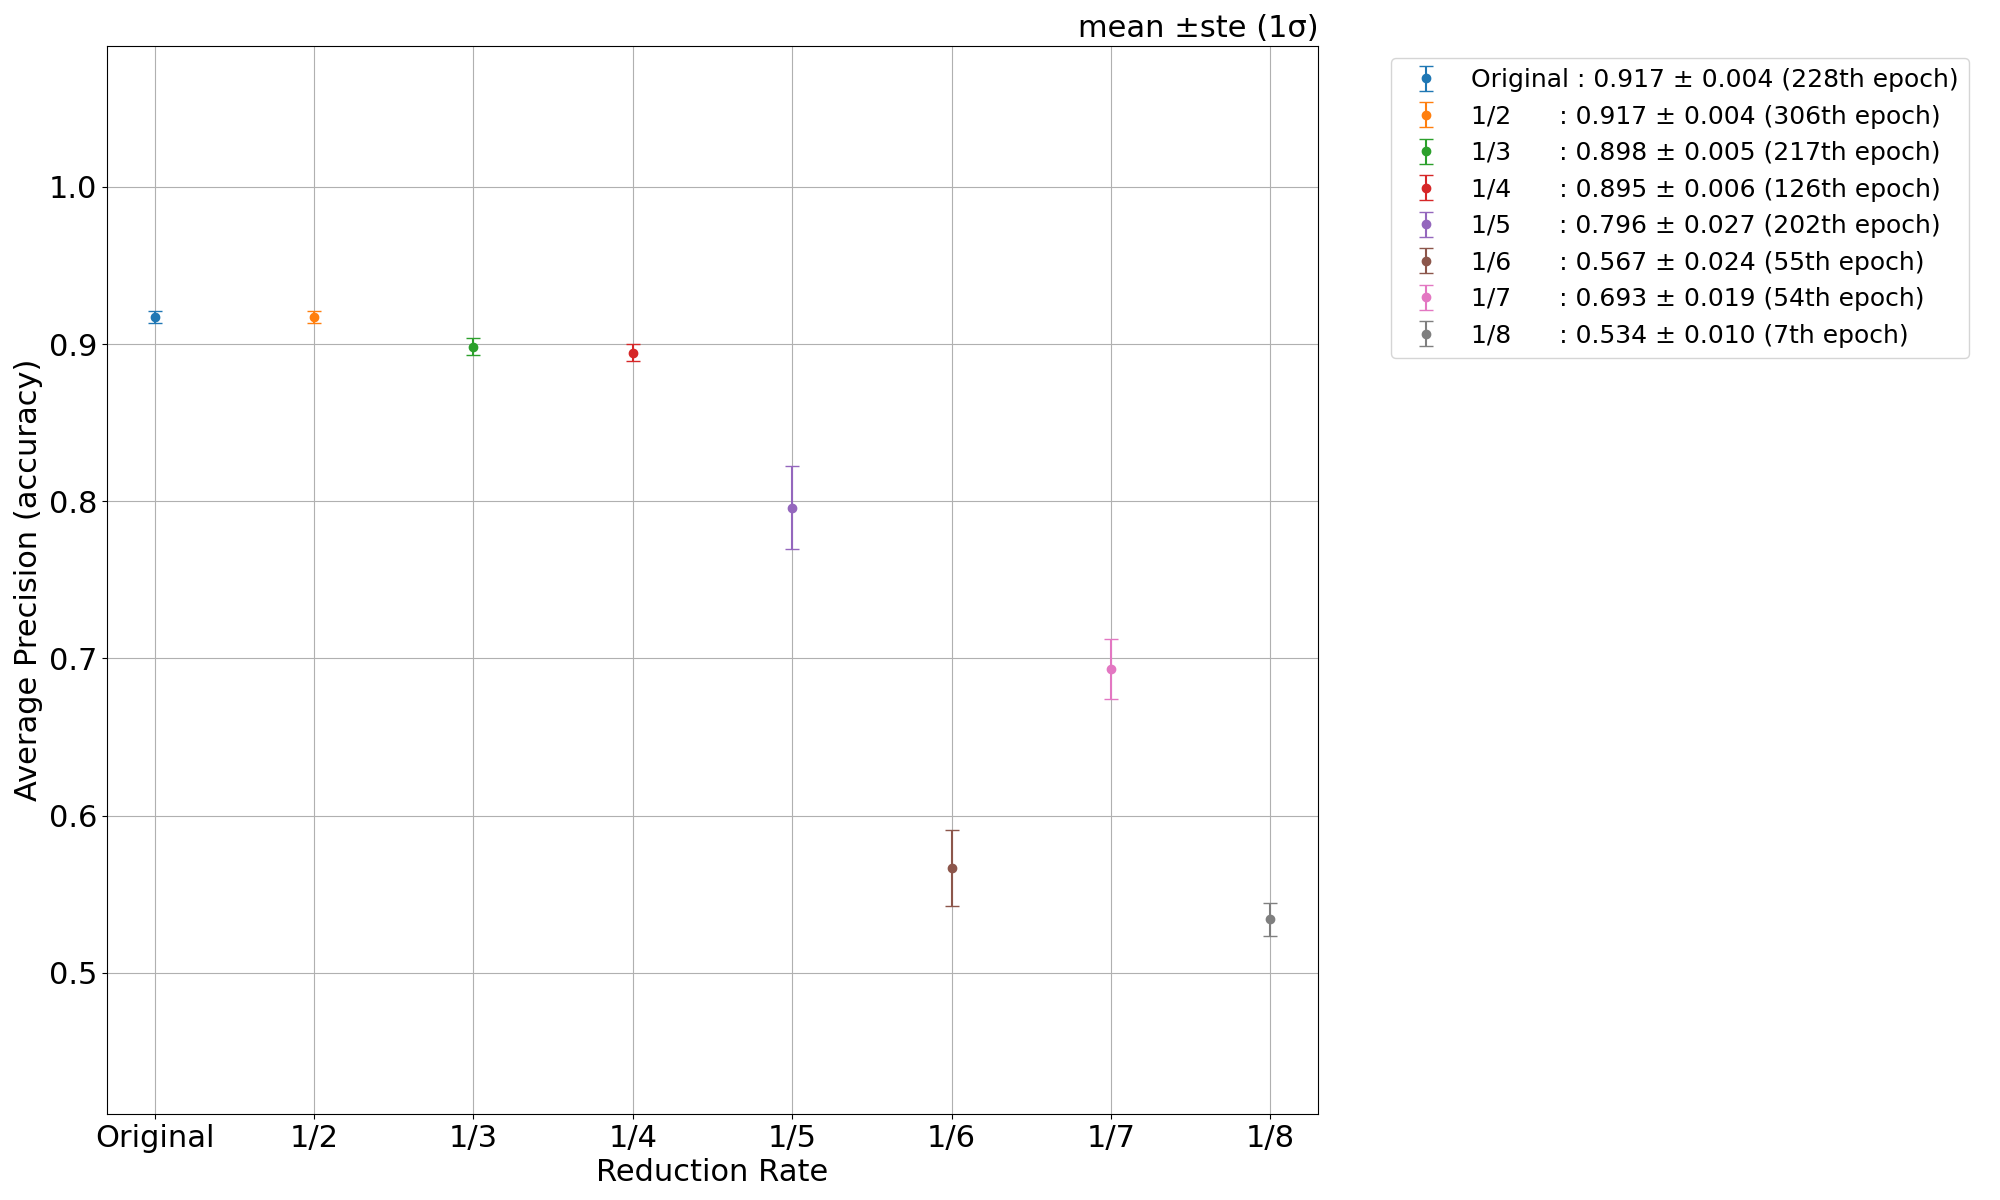
\includegraphics[width=16cm]{images/5syou/print_errorbar/nearest/acc_with_errorbar_syuron5_nearest_900epoch_30run_300_acc_max_ste1sigma.png}
%   \caption{最近傍補間によって内挿された,縮小データに対するモデルの予測結果(1ste)}
%   \label{fig:nearest_300_1ste}
% \end{figure}

% \begin{figure}[H]
%   \centering
%   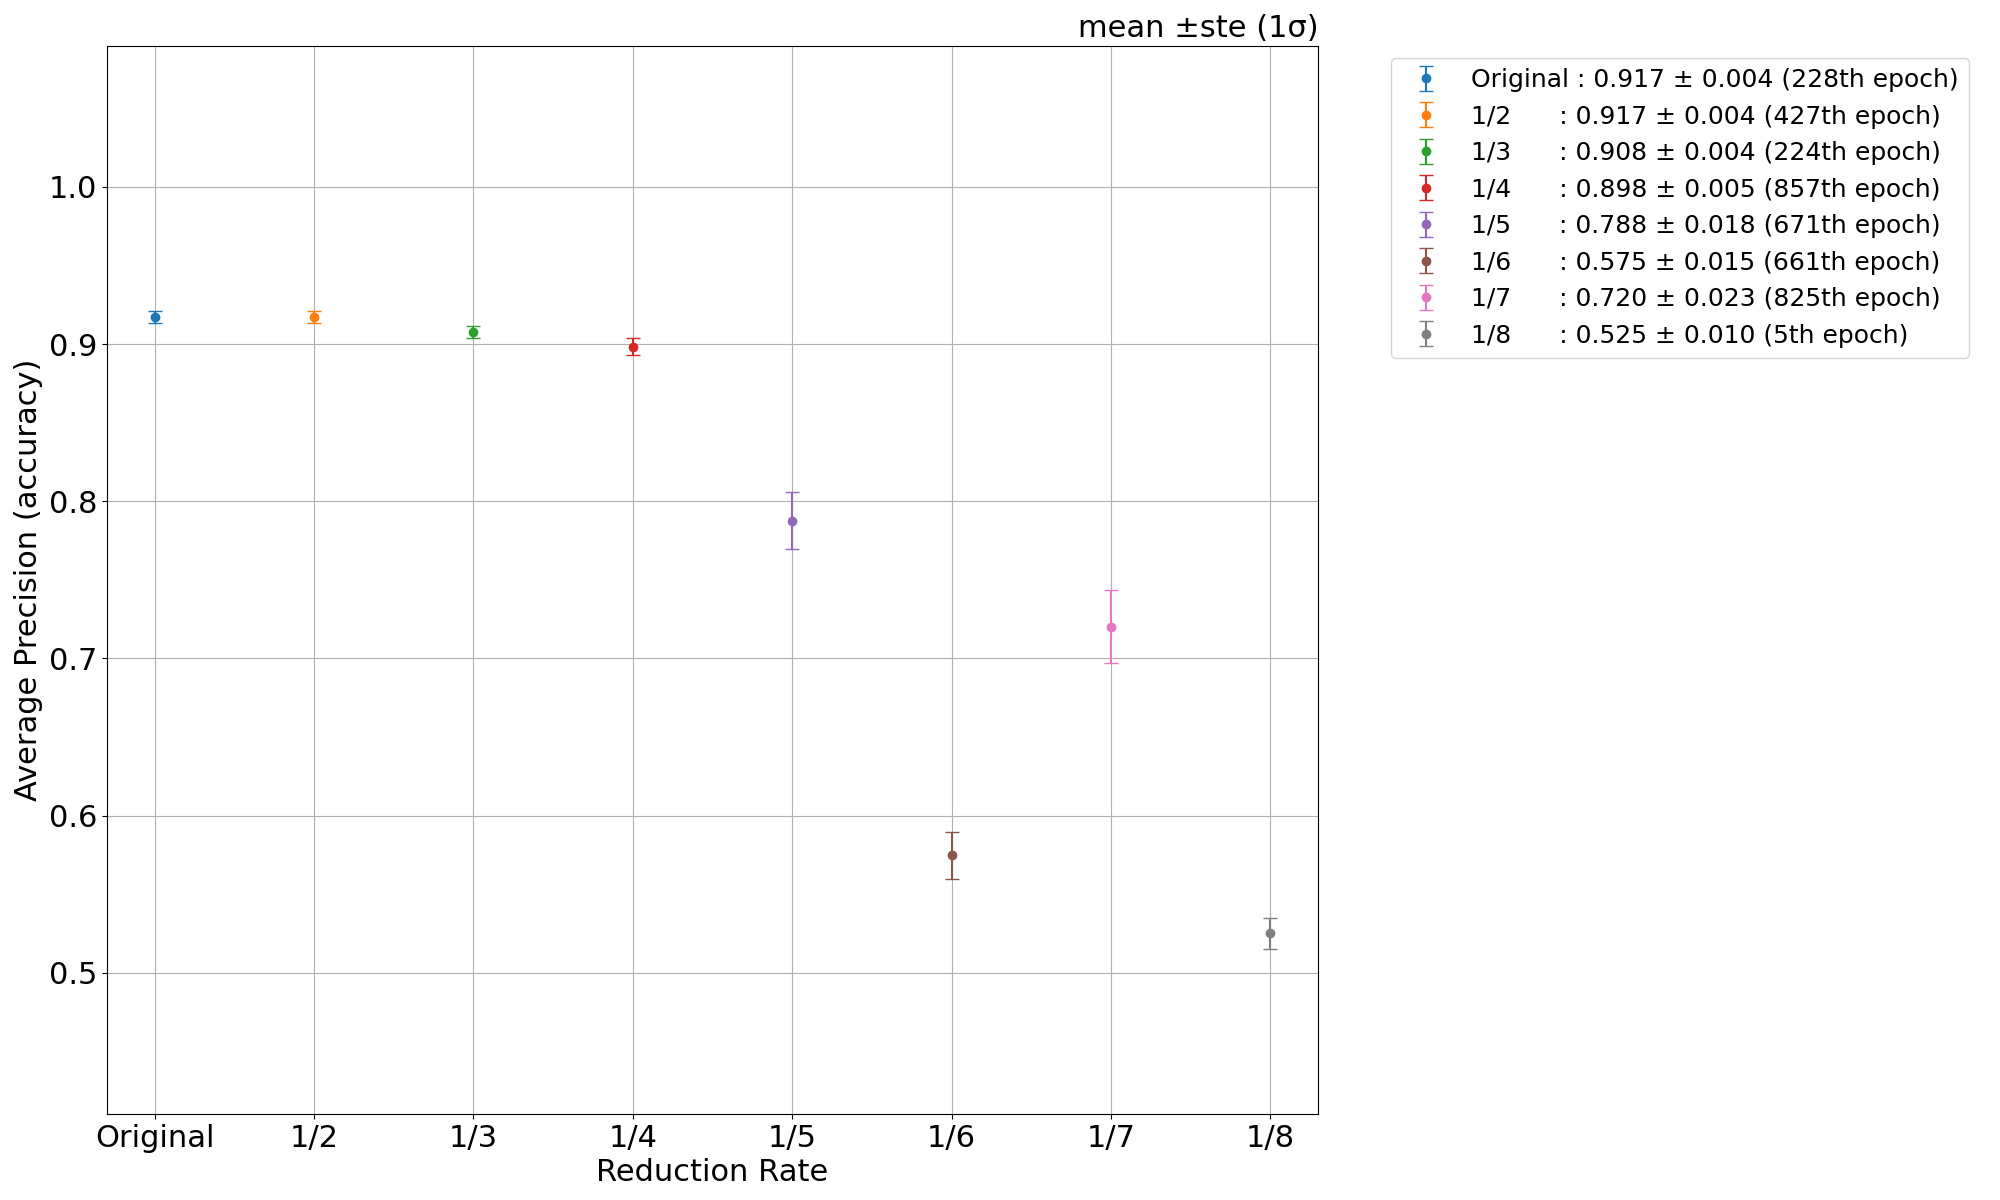
\includegraphics[width=16cm]{images/5syou/print_errorbar/linear/acc_with_errorbar_syuron5_linear_900epoch_30run_300_acc_max_ste1sigma.png}
%   \caption{バイリニア補間によって内挿された,縮小データに対するモデルの予測結果(1ste)}
%   \label{fig:linear_300_1ste}
% \end{figure}
 
% \begin{figure}[H]
%   \centering
%   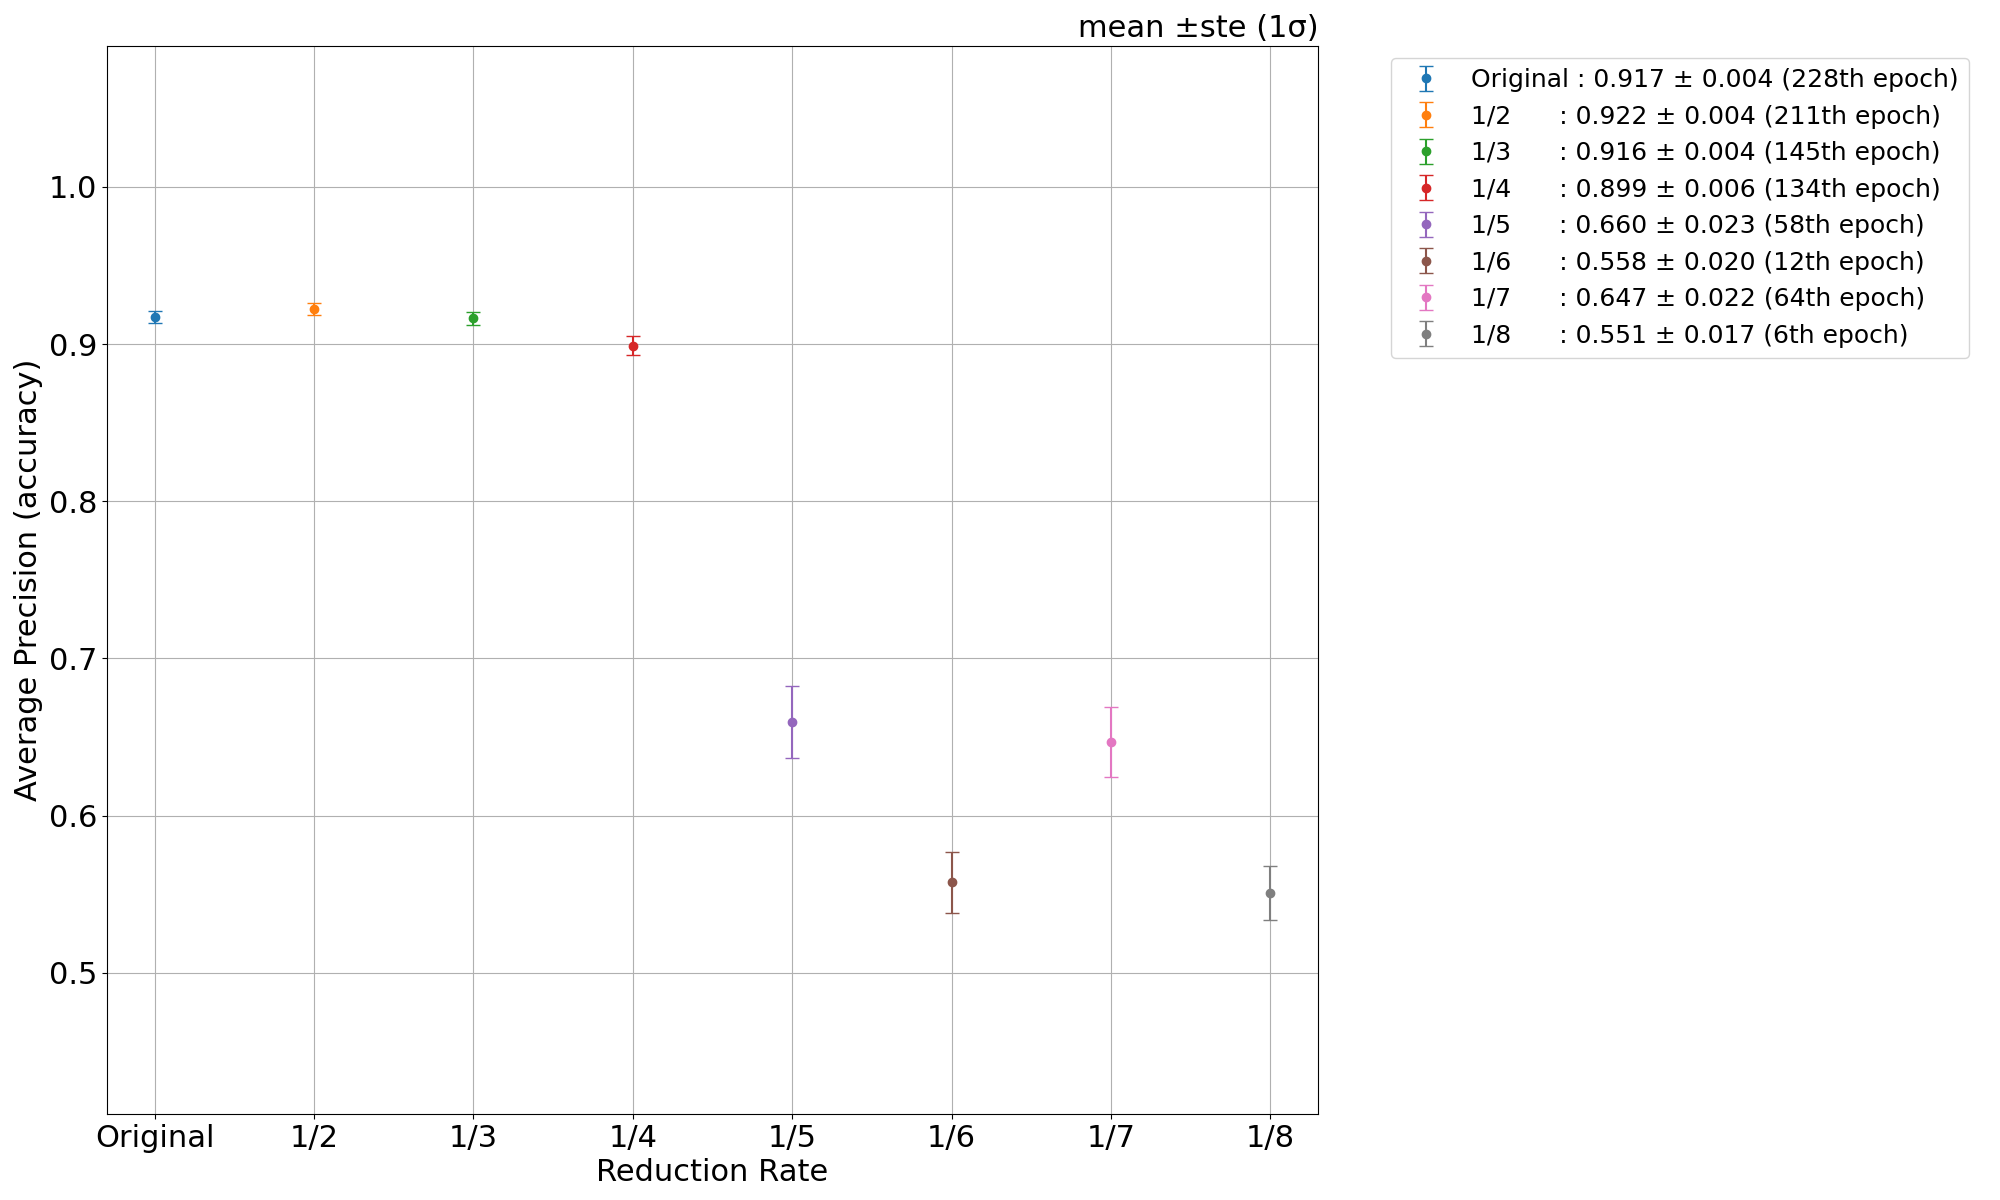
\includegraphics[width=16cm]{images/5syou/print_errorbar/cubic/acc_with_errorbar_syuron5_cubic_900epoch_30run_300_acc_max_ste1sigma.png}
%   \caption{バイキュービック補間によって内挿された,縮小データに対するモデルの予測結果(1ste)}
%   \label{fig:cubic_300_1ste}
% \end{figure}

\begin{table}[H]
  \centering
	\caption{最近傍補間によって拡大したテストデータに対する予測精度(1標準誤差)}
  \begin{tabular}{|c|c|}
		\hline
    & 1ste \\ \hline
    Original & $0.004$ \\ \hline
    1/2 & $0.004$ \\ \hline
    1/3 & $0.005$ \\ \hline
    1/4 & $0.006$ \\ \hline
    1/5 & $0.027$ \\ \hline
    1/6 & $0.024$ \\ \hline
    1/7 & $0.019$ \\ \hline
    1/8 & $0.010$ \\ \hline
  \end{tabular}
  \label{tb:accs_4_2_nearest_1ste}
\end{table}

\begin{table}[H]
  \centering
	\caption{バイリニア補間によって拡大したテストデータに対する予測精度(1標準誤差)}
  \begin{tabular}{|c|c|}
		\hline
    & 1ste \\ \hline
    Original & $0.004$ \\ \hline
    1/2 & $0.004$ \\ \hline
    1/3 & $0.004$ \\ \hline
    1/4 & $0.005$ \\ \hline
    1/5 & $0.018$ \\ \hline
    1/6 & $0.015$ \\ \hline
    1/7 & $0.023$ \\ \hline
    1/8 & $0.010$ \\ \hline
  \end{tabular}
  \label{tb:accs_4_2_linear_1ste}
\end{table}

\begin{table}[H]
  \centering
	\caption{バイキュービック補間によって拡大したテストデータに対する予測精度(1標準誤差)}
  \begin{tabular}{|c|c|}
		\hline
    & 1ste \\ \hline
    Original & $0.004$ \\ \hline
    1/2 & $0.004$ \\ \hline
    1/3 & $0.004$ \\ \hline
    1/4 & $0.006$ \\ \hline
    1/5 & $0.023$ \\ \hline
    1/6 & $0.020$ \\ \hline
    1/7 & $0.022$ \\ \hline
    1/8 & $0.017$ \\ \hline
  \end{tabular}
  \label{tb:accs_4_2_cubic_1ste}
\end{table}



\newpage
\section{分類精度の使用天体数依存性}
% 予測精度を高く保ったまま,学習データの枚数をなるべく少なくする方が好ましい.理由としては,一つの天体画像データセットが完成するのには10年もしくはそれ以上の時間がかかり,またそれに対する形態分類付けが完了するには更に多くの時間がかかるからである.そのため,今度登場するであろう高解像度データセットの完成を待たずある程度の高解像度天体データが撮影された時点で,それらを用い高精度の分類モデルを学習し,既存の低解像度データセットに対し形態分類の予測を適用することが将来展望の構想である.
% したがって本研究にて,形態分類の精度を高く保ったまま,どのくらいの使用天体数の少なさなら使えるかを検証することは,将来展望を議論するのに有用である.
この節では,クラスごとの使用天体数が300天体で十分かどうか(学習データ内のデータの多様性が足りているか)を検証する.具体的には,クラスごとの使用天体数をそれぞれ500, 800, 1000天体とし,モデルの学習・テストを行う.5.2節で行っていた300天体の結果も合わせて,使用天体数300, 500, 800, 1000天体で行った実験におけるモデルの予測結果を,テストデータに対する予測のaccuracyをもって比較し,以下を検証する.
\begin{quote}
 \begin{itemize}
  \item テストデータに対する予測のaccuracyに変化はあるのか,変化幅はどのくらいか
  \item ''Original''の結果と同程度の分類精度を達成するテストデータの縮小倍率に,差が生じるか
 \end{itemize}
\end{quote}

\subsection{実験条件}
使用する天体は4.3節および5.2節での実験と同様に,不確か天体を除いた5,618天体を母集団とし,クラスごとにそれぞれ500,800および1000天体を使用した.
また使用する画像データに関しては5.2節同様に,学習データにはSDSSの切り出し画像,テストデータにはSDSSの切り出し画像を縮小した画像をそれぞれ用いた.

モデルの学習期間は,5.2節と同様の理由で900epochとした.

学習させたモデルは第4章および5.2節と同様に30回の学習を行い,平均値および標準偏差を導出した.

% モデルの学習期間は900epochとした.これは,すべての縮小データの縮小倍率にて,モデルが学習しきる期間,すなわちテストデータに対するaccuracyが上がりきるepoch数が900epochであったからである.

\subsection{実験結果}
銀河切り出し画像を1/2, 1/3, ..., 1/8倍に縮小した縮小データに対する,形態分類モデルの予測結果の図を図\ref{fig:nearest_num_of_gal_comparison_1std}から図\ref{fig:cubic_num_of_gal_comparison_1std}に示す.これらの図は5.2節の実験結果である図\ref{fig:inter_comparison_300_1std}と同様の形式である.accuracyについては,30回実行における平均値と1標準偏差を示している.凡例には,エラーバーの各色とクラスごとの使用天体数の対応付けが示されている.

\begin{figure}[H]
  \centering
  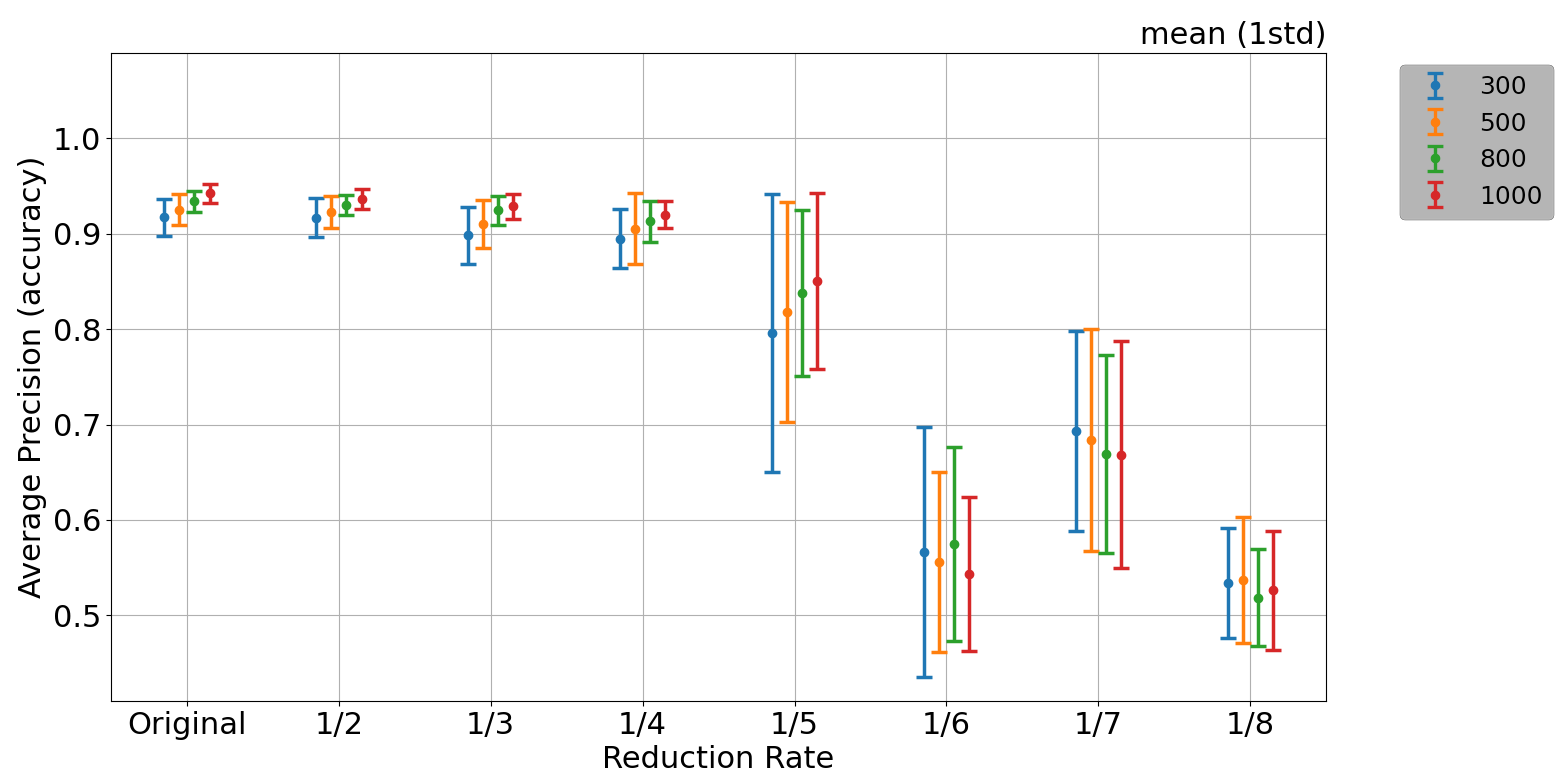
\includegraphics[width=1.0\hsize, keepaspectratio]{images/5syou/print_errorbar/nearest/acc_with_errorbar_syuron5_nearest_900epoch_30run_num_of_gal_comparison_acc_max_std1sigma.png}
  \caption{最近傍補間によって内挿された,縮小データに対するモデルの予測結果}
  \label{fig:nearest_num_of_gal_comparison_1std}
\end{figure}

\begin{figure}[H]
  \centering
  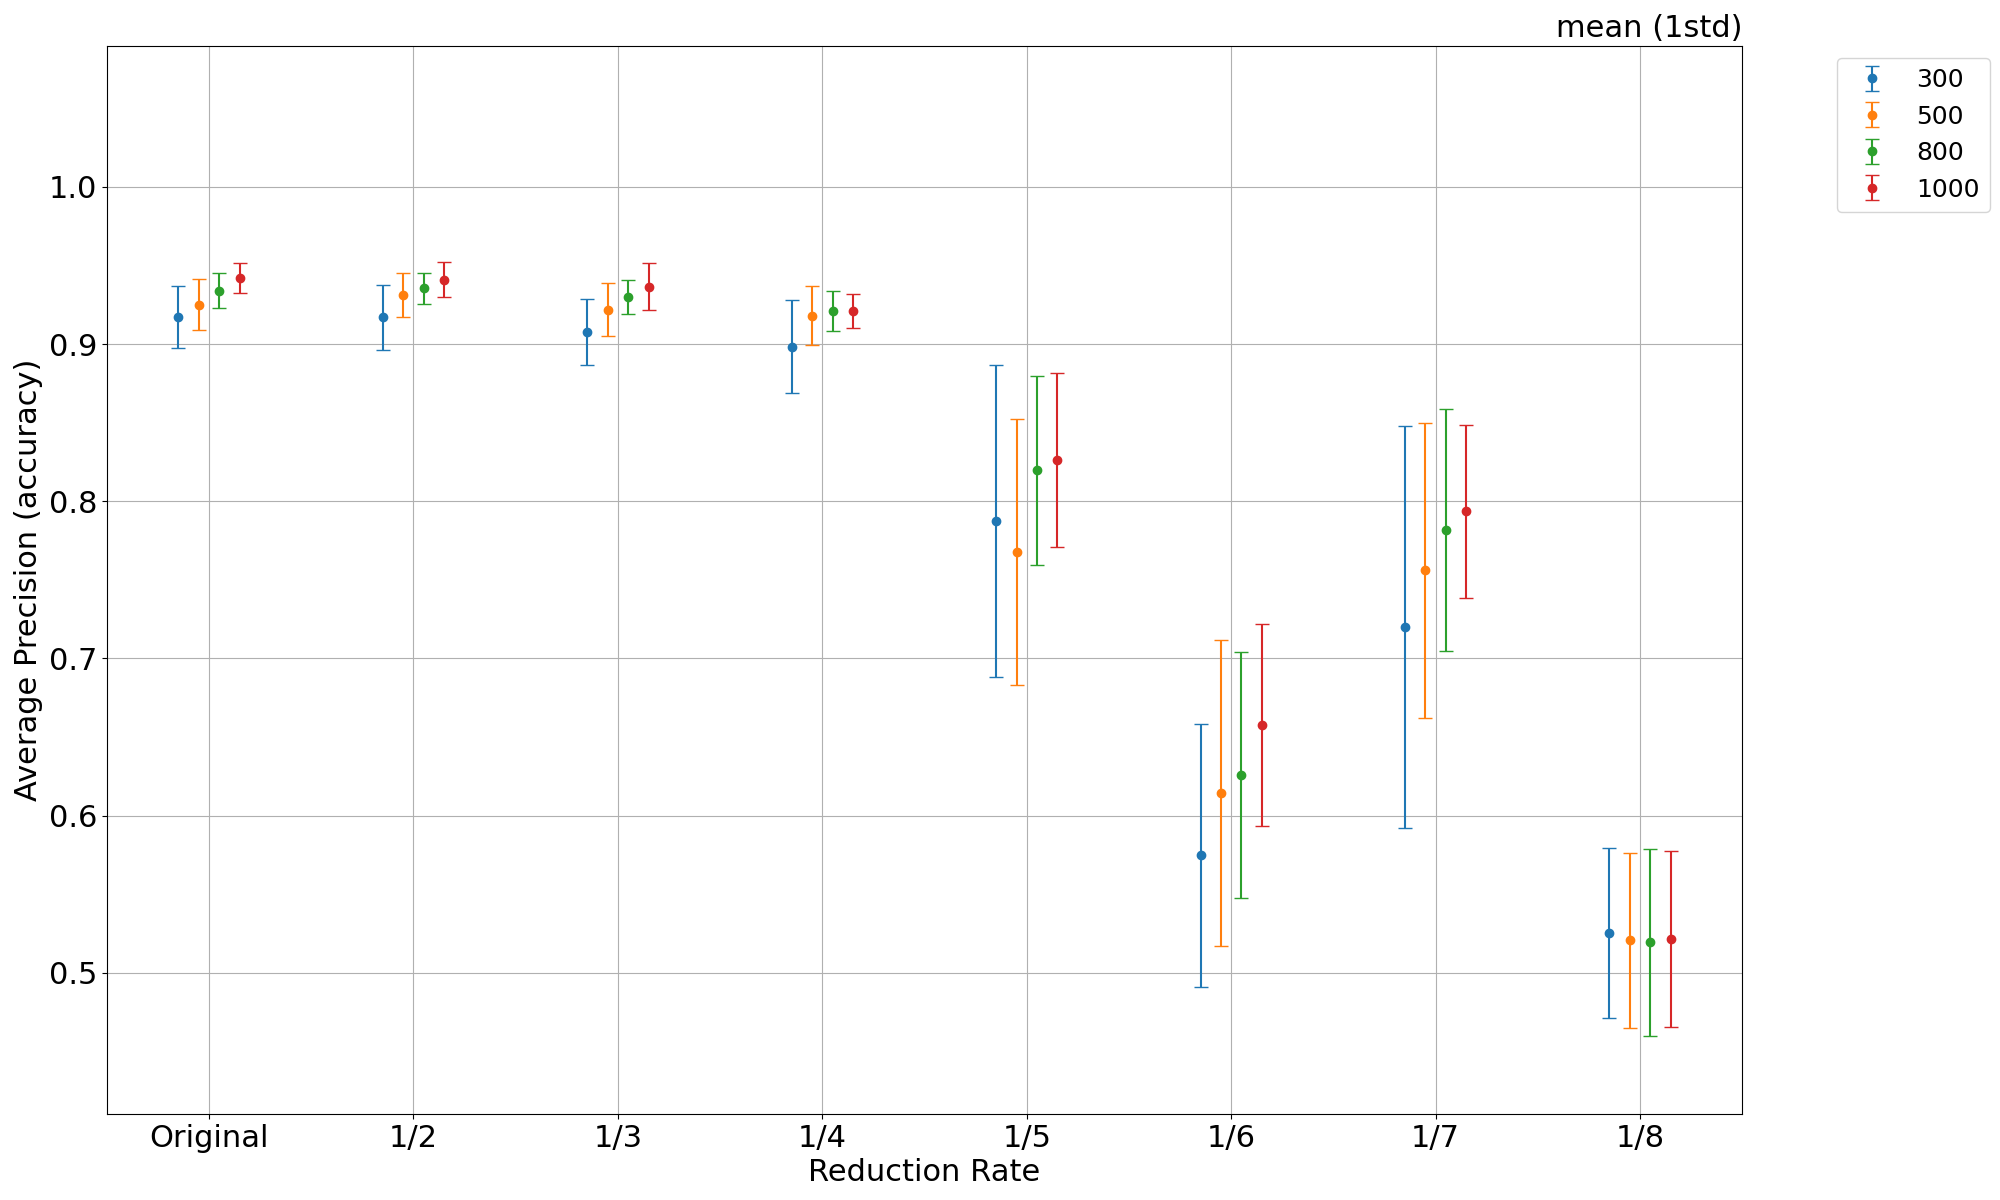
\includegraphics[width=1.0\hsize, keepaspectratio]{images/5syou/print_errorbar/linear/acc_with_errorbar_syuron5_linear_900epoch_30run_num_of_gal_comparison_acc_max_std1sigma.png}
  \caption{バイリニア補間によって内挿された,縮小データに対するモデルの予測結果}
  \label{fig:linear_num_of_gal_comparison_1std}
\end{figure}

\begin{figure}[H]
  \centering
  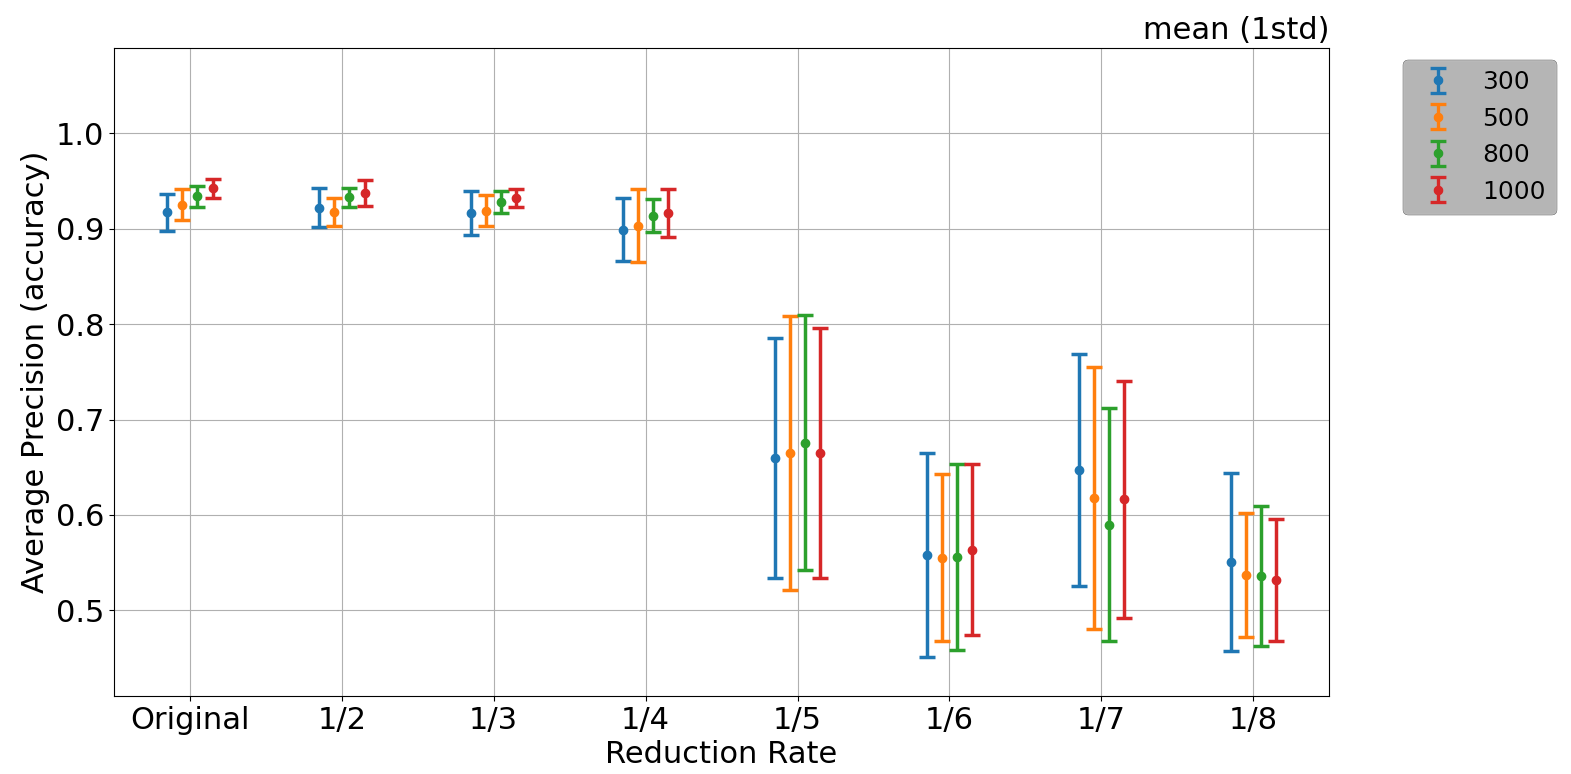
\includegraphics[width=1.0\hsize, keepaspectratio]{images/5syou/print_errorbar/cubic/acc_with_errorbar_syuron5_cubic_900epoch_30run_num_of_gal_comparison_acc_max_std1sigma.png}
  \caption{バイキュービック補間によって内挿された,縮小データに対するモデルの予測結果}
  \label{fig:cubic_num_of_gal_comparison_1std}
\end{figure}

\subsubsection{使用天体数増加によるaccuracyの変化}
使用天体数を増やすことで補間方法によらず,縮小倍率が1/2倍から1/4倍の縮小画像データに対する予測のaccuracyの標準偏差の値が減少した.特に使用枚数が300枚と1000枚の結果を比較すると,標準偏差の値がおよそ半減していることが図\ref{fig:nearest_num_of_gal_comparison_1std}から図\ref{fig:cubic_num_of_gal_comparison_1std}より読み取れる.
しかしながら,標準偏差の値は減少するものの,縮小倍率が1/2から1/4倍においてクラスごとの使用天体数による有意差は見受けられなかった.


\subsubsection{内挿方法間での比較}
内挿方法の間で,クラスごとの天体使用数を増加させた際に見受けられる,テストデータに対するaccuracyを比較する.なお,縮小倍率1/2倍から1/4倍のデータに対する予測結果は前段落である\textbf{使用天体数増加によるaccuracyの変化}で述べたので,ここからは縮小倍率が1/5倍以上のデータに対する結果を比較する.

最近傍補間によってテストデータの内挿を行った場合,クラスごとの天体使用数を増加させることで,縮小倍率1/5倍のデータに対する予測のaccuracyの標準偏差減少が見受けられる.しかしながら,標準偏差の減少量は1/2倍から1/4倍の縮小倍率データに対する予測のaccuracyと比べると,それほど大きくないことが分かる.

バイリニア補間によってテストデータの内挿を行った場合,クラスごとの天体使用数を1000天体まで増やしても,1/5倍から1/8倍の縮小倍率データに対する予測のaccuracyが0.9を超えなかった.しかしながら,クラスごとの天体使用数を増加させることで,縮小倍率が1/5倍から1/7倍のテストデータに対する予測のaccuracyの精度改善が見込めた.なお1/8倍の縮小倍率に対する形態分類は,クラスごとの天体使用数および内挿方法を問わずaccuracy0.5付近を記録した.このため,学習データとテストデータとの間の解像度差が1/8倍である場合,深層学習モデルによる形態予測が行えないのではないかと思われる.

バイキュービック補間によってテストデータの内挿を行った場合,クラスごとの天体使用数を1000天体まで増やしても,1/5倍から1/8倍の縮小倍率データに対する予測のaccuracyが0.9を超えず,またaccuracyの標準偏差に改善が見られなかった.

\subsubsection{使用可能なデータセット間の解像度差について}
図\ref{fig:nearest_num_of_gal_comparison_1std}から図\ref{fig:cubic_num_of_gal_comparison_1std}より,内挿方法を問わず,クラスごとの天体使用数を300,500,800,1000のいずれに定めても,縮小倍率が1/4倍までの縮小データに対する予測のaccuracyが,Originalの結果と同程度を記録することが読み取れる.このことから今回の実験条件の範囲内であれば,内挿方法・クラスごとの使用天体数によらず,学習データとテストデータの解像度差が1/4までならば使用可能であることが分かった.
また\textbf{内挿方法間での比較}にて,縮小倍率が1/4倍までの縮小データに対する予測では,銀河種ごとの天体使用数を増加させることで内挿方法によらず予測精度が向上することが分かった.このことから,学習データとテストデータの解像度差が1/2倍から1/4倍ほどである2値銀河形態分類は,モデルの学習の上振れを期待せずとも,高精度の形態予測を期待できる分類問題であると思われる.

次に,学習データとテストデータの解像度差が1/5倍より大きい場合について述べる.最近傍補間によってテストデータを内挿する場合,解像度差が1/5倍のとき,銀河種ごとの天体使用数を増やすことで誤差区間が減少する.しかし,最も多い天体数である使用天体数1000天体においても,Originalの結果と同程度を記録しなかった.このことから,モデルの学習が上振れることを期待する必要があるため使用不可な解像度差であると判断した.また,図\ref{fig:linear_num_of_gal_comparison_1std},図\ref{fig:cubic_num_of_gal_comparison_1std}より,バイリニア補間,およびバイキュービック補間においては,Originalの結果と同程度を記録しないことが読み取れる.

したがって,学習データとの解像度差が1/5倍より大きいテストデータは使用不可であることがわかった.

\newpage
\section{議論}
\subsubsection{どの補間フィルタを用いるべきか}
第5章では学習データに高解像度,テストデータに低解像度の画像データを使用していた.深層学習モデルに入力する画像データは全て同じサイズである必要があるため,今回の実験ではテストデータである低解像度画像の拡大を行った.ここで,本研究で扱った「学習データとテストデータにおける天体画像に解像度差がある分類問題」というテーマにて,3つの画像拡大手法(最近傍補間・バイリニア補間・バイキュービック補間)のうち,どれを使うべきかを考察する.

まず,第5章にて使用可能と定義した,学習データとテストデータとの間の解像度差が1/2倍から1/4倍の状況でモデルの学習・それによる予測を行う場合について,図\ref{fig:nearest_num_of_gal_comparison_1std}から図\ref{fig:cubic_num_of_gal_comparison_1std}より,どの天体使用数においても,3つの拡大手法でのaccuracyは同程度を記録している.このことから,学習データとテストデータとの間の解像度差が1/2倍から1/4倍の状況でモデルの学習・それによる予測を行う場合,これら3手法のどれを使用しても高精度の予測が行えると考えられる.ただし図\ref{fig:cubic_num_of_gal_comparison_1std}より,バイキュービック補間は使用天体数を増やした際のaccuracyの標準偏差低下の恩恵を受けづらいことが読み取れる.

次に,3つの拡大手法の処理にかかる時間を考える.時間計測を行うため,SDSSから取得した銀河切り出し画像を1/8倍に縮小した縮小画像のうち,渦巻銀河50天体・楕円銀河50天体について拡大処理を実行した.拡大処理は各手法にてそれぞれ10000回ずつを10周実行し,100天体の拡大にかかった時間の平均値および1標準偏差を導出した.
表\ref{tb:calc_cost_by_interpolation}にそれぞれの拡大手法が100天体の拡大処理にかかる時間を示す.表より,最近傍補間が最も処理が軽く,バイリニア補間が2番目,バイキュービック補間が3番目に処理に時間がかかることが読み取れる.

上で述べた2点を総合的に考慮すると,今回のような実験条件,すなわち学習データとテストデータの解像度差が1/4倍まででモデルの作成を行う場合は,分類精度は他2手法と差がなく画像拡大処理が最も軽い最近傍補間が望ましいと考えられる.


\begin{table}[htbp]
  \centering
	\caption{各補間フィルタによる画像拡大の計算時間}
  \begin{tabular}{|c|c|}
		\hline
     & mean(1std) \\ \hline
    最近傍補間 & $247\mu s \pm 2.25\mu s$ \\ \hline
    バイリニア補間 & $378\mu s \pm 5.37\mu s$ \\ \hline
    バイキュービック補間 & $1.48ms \pm 7.74\mu s$ \\ \hline
  \end{tabular}
  \label{tb:calc_cost_by_interpolation}
\end{table}

% \subsubsection{学習データとテストデータとの間の解像度差が1/6および1/7の際の,テストデータに対する予測accuracyの挙動}
% 第5章にて使用天体数・内挿方法を問わず共通の傾向であった,「縮小倍率が1/7倍の縮小データに対する予測精度が,縮小倍率1/6倍の予測精度より高い」事に対し,考察を行う.

% 一般的に,テストデータの解像度が低ければ低いほど,分類モデルによる予測精度は低くなると考えられる.図\ref{fig:nearest_num_of_gal_comparison_1std}から図\ref{fig:cubic_num_of_gal_comparison_1std}においても,縮小倍率が1/2倍から1/6倍においては上記の傾向が見受けられる.しかしながら,1/7倍の縮小倍率に対する予測精度は,1/2倍から1/6倍にて見受けられた傾向から逸脱している.この傾向に対し,考察を行う.

% 1/6倍, 1/7倍の縮小画像に対する画像拡大例を図\ref{fig:1_6and1_7}に示す.図\ref{fig:1_6and1_7}より,拡大手法によって生成される画像が,見かけではかなり異なることが分かる.しかし,図\ref{fig:nearest_num_of_gal_comparison_1std},図\ref{fig:linear_num_of_gal_comparison_1std}を比較すると,拡大手法によって縮小倍率1/6倍と縮小倍率1/7倍のaccuracyの挙動に大きな差はないことが分かる.ここで,1/6倍,1/7倍の縮小画像(図\ref{fig:1_6and1_7}の左下)を見ると,画像内の最も明るいピクセルが存在する場所に差があることが分かる.1/6倍の縮小画像では中央より右下,1/7倍の縮小画像では中央が一番明るいピクセルであることが読み取れる.このことから,平均画素法による縮小の際,何らかの形で銀河の形態的特徴が損失している可能性がある.そしてこの形態的特徴損失により,学習データとテストデータとの間の解像度差が1/6および1/7の際の,テストデータに対する予測accuracyの挙動に影響を及ぼしていると思われる.

% \begin{figure}[htbp]
%  \centering
%  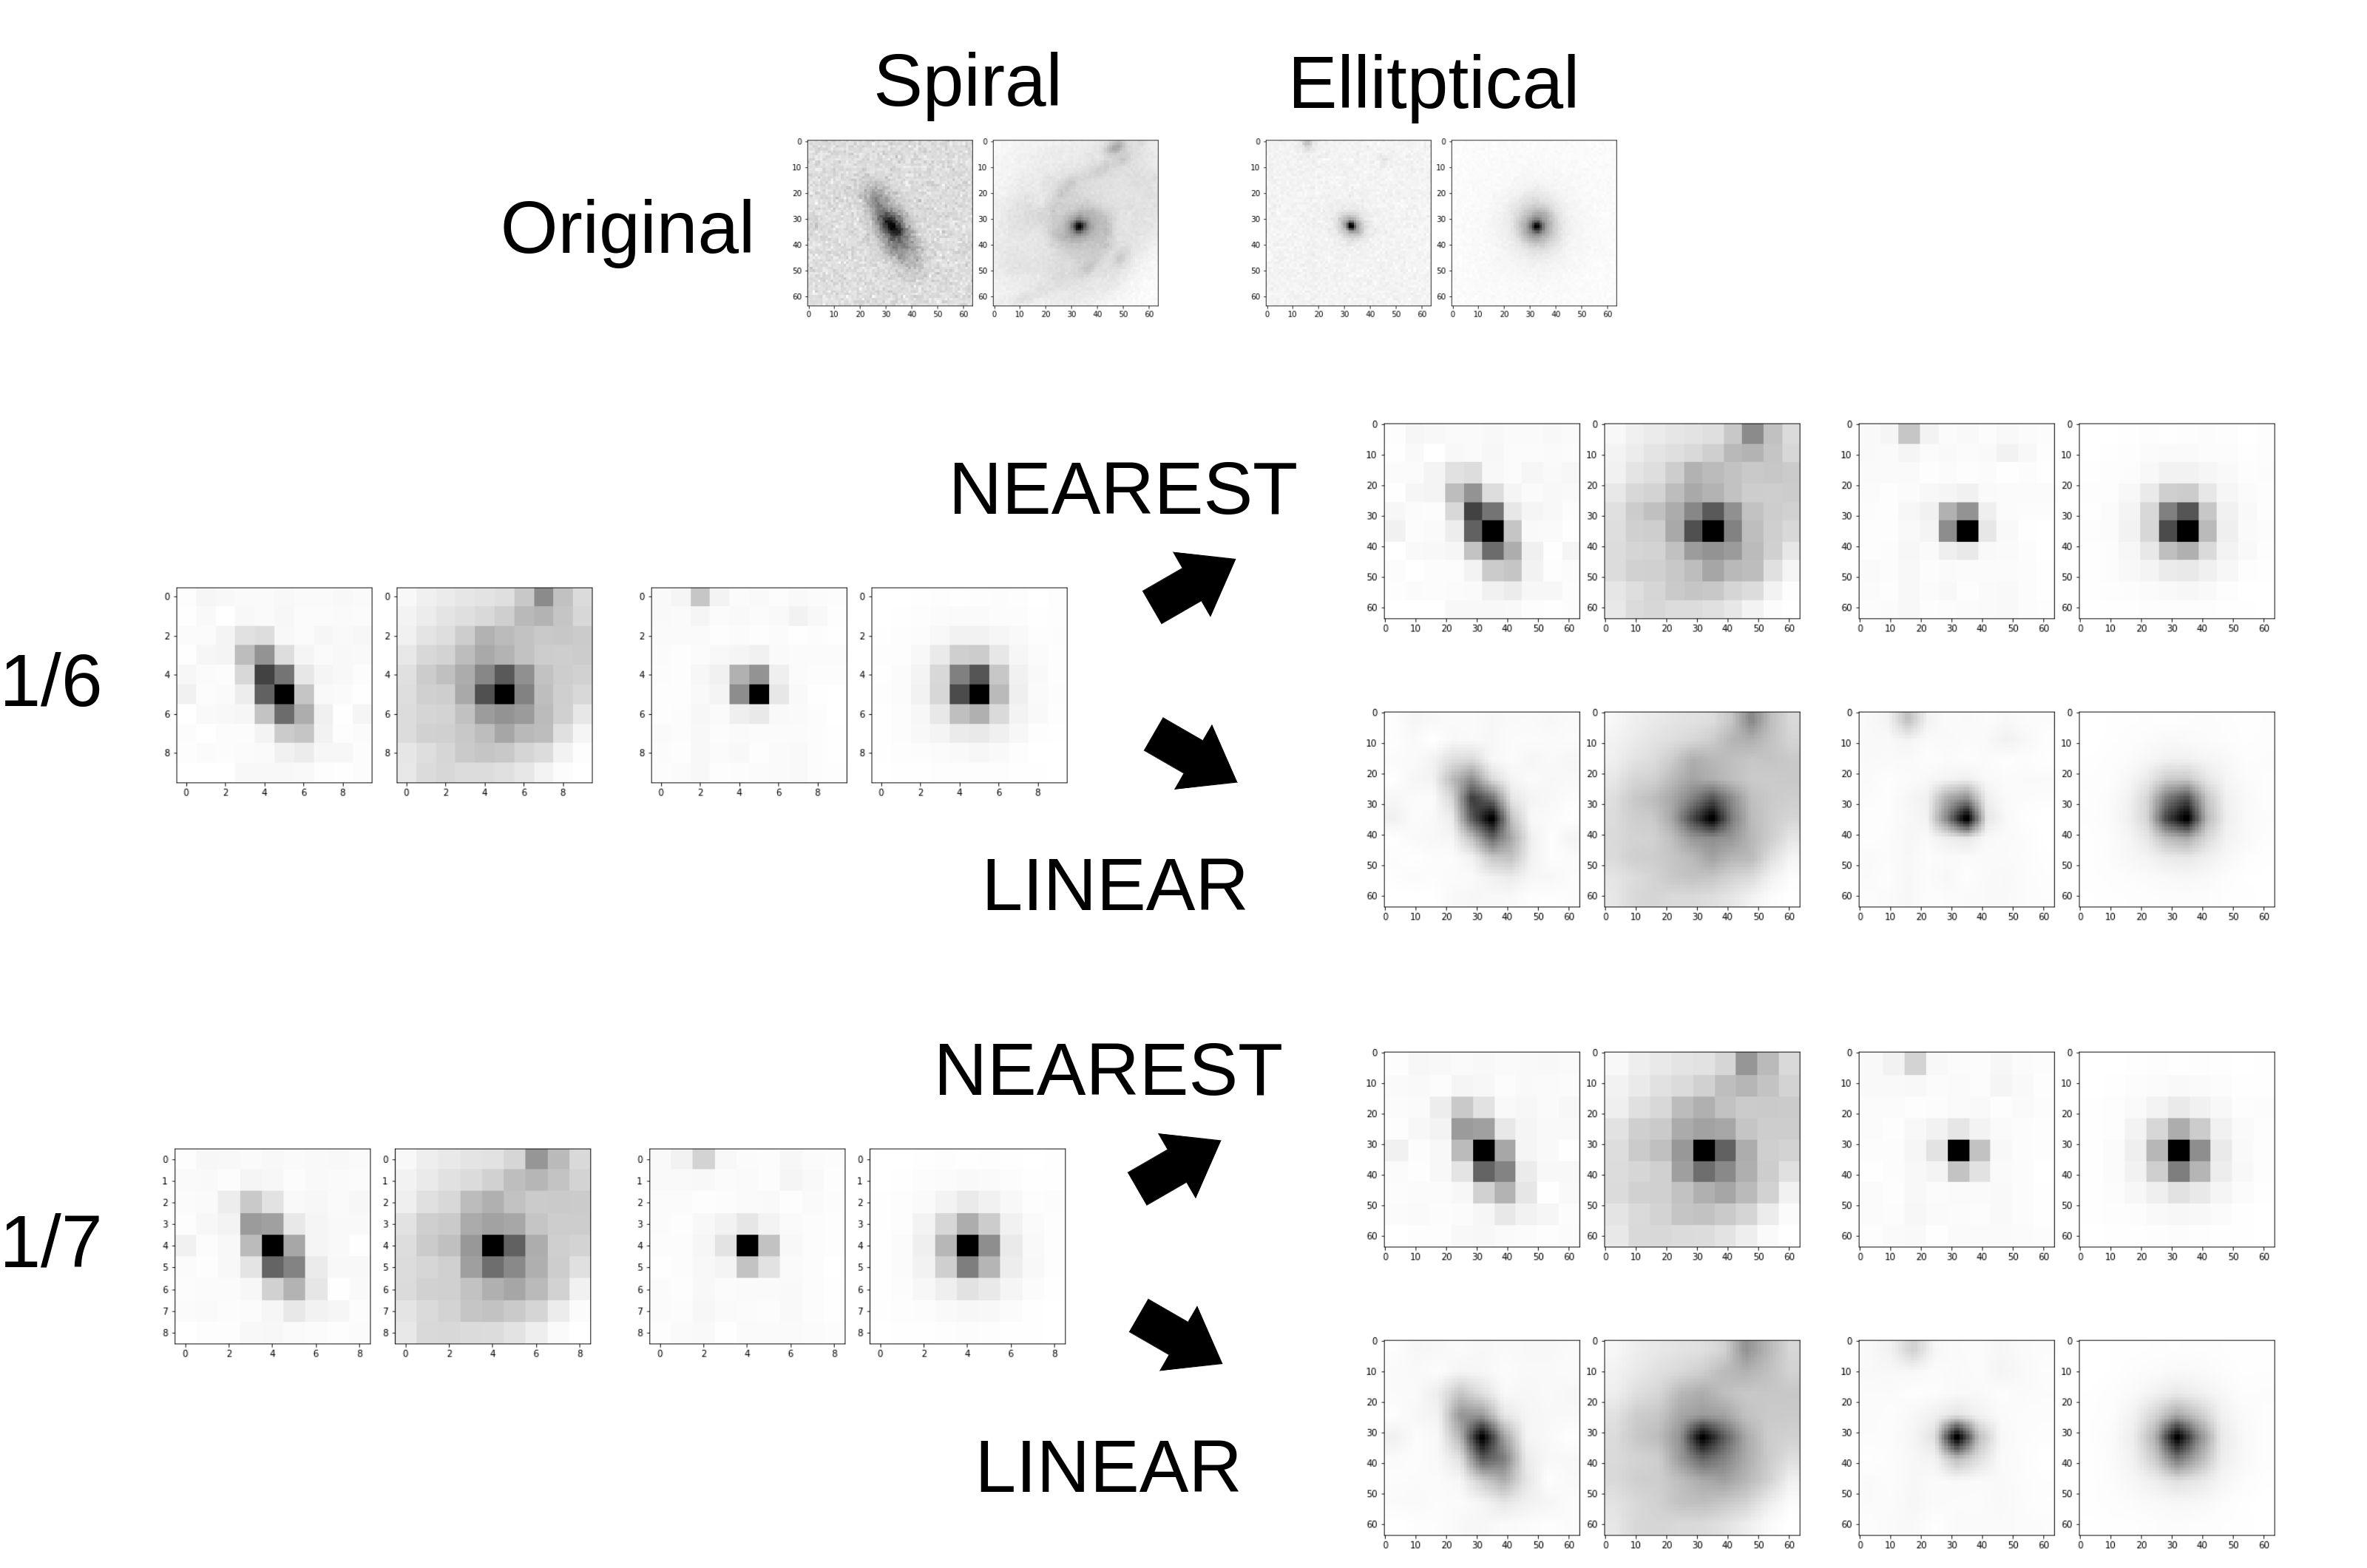
\includegraphics[width=1.0\hsize, keepaspectratio]{images/5syou/syuron_5syou_kakudai/ver1/5syou_giron_1_6and1_7.png}
%  \caption{1/6倍, 1/7倍の縮小画像に対する画像拡大例(最近傍補間・バイリニア補間)}
%  \label{fig:1_6and1_7}
% \end{figure}


\subsubsection{クラスごとの使用天体数をどう設定するべきか}
次に,「学習データとテストデータにおける天体画像に解像度差がある分類問題」というテーマにて,クラスごとの使用天体数をどうするべきかについて考察する.
図\ref{fig:nearest_num_of_gal_comparison_1std}から図\ref{fig:cubic_num_of_gal_comparison_1std},および5.3節の\textbf{使用可能なデータセット間の解像度差について}で述べた結果より,今回のような実験条件,すなわち渦巻銀河と楕円銀河の2値分類問題で使用可能と定義した1/2倍から1/4倍の学習データ・テストデータ間の解像度差においては,クラスごとの使用天体数は300天体から1000天体の間の数であれば何天体としてもよいと思われる.これは,クラスごとの使用天体数を300天体から1000天体のいずれに設定しても,使用可能と定義されるテストデータの縮小倍率の範囲に差が生じなかったからである.

しかしながら,クラスごとの使用天体数を増加させることでテストデータに対する予測のaccuracyの期待値は増加するため,より高い予測精度が求められる場合にはクラスごとの使用天体数は増加させたほうが良いと思われる.

この章では,「学習データとテストデータとの間に解像度差があるデータセットにて形態分類モデルの作成が行えるか」の検証を行うため,2つの実験を行った.

クラスごとの使用天体数が300天体の場合,学習データとテストデータとの間の解像度差が1/4までならば,画像拡大方法によらず使用可能,すなわち学習データとテストデータの解像度が揃っている状況での予測結果である”Original” と同程度の精度での分類を達成した.

クラスごとの使用天体数を増加させた際,テストデータに対する予測のaccuracyの挙動は画像拡大方法によって差が生じた.一方で,使用可能と定義される学習データとテストデータ間の解像度差の範囲に差が生じることはなかった.したがって,学習データとテストデータとの間に解像度差がある状況での渦巻銀河と楕円銀河の2値分類問題を扱う場合,
画像拡大方法を問わず,使用天体数を300天体から1000天体のいずれでも,1/4倍の解像度差までならば深層学習モデルによる分類が可能であることが示された.

画像拡大方法によってテストデータに対する予測のaccuracyが異なる挙動を見せることから,モデルへの内挿方法を模索することで,更なる精度改善,および本研究では使用不可と判断した学習データとテストデータとの間の解像度差においても,使用可能となる可能性がある.

\newpage
\chapter{将来課題}
\section{本研究のまとめ}
本研究の将来展望は,高空間分解能観測装置データを用いてモデル学習を行うことで,既存の低空間分解能データセットに対し更なる高精度形態分類を提供するというものである.この将来展望が実現できる可能性を検証するため,本研究では第4章,第5章にて将来展望の前段階となる実験群を行った.その結果,深層学習による銀河形態分類の渦巻銀河・楕円銀河に分類する2値分類問題において,学習データとテストデータとの間に1/4倍までの画像解像度差が生じていても,解像度差がない場合の予測精度であるaccuracy$0.917 \pm 0.020$と同程度の精度の予測が提供できることが分かった.本論文での実験結果によって深層学習モデルの予測を,学習データより低い解像度のデータに対し適用が行えることを示したため,今後は将来展望である「異なる観測装置データの組み合わせを行い,深層学習による銀河形態分類」に取り組む.

一方で,SDSSとGZを組み合わせた深層学習による形態分類の更なる精度向上など,多くの将来課題が残されている.6.2節ではそれらについて言及を行う.

\section{将来課題}
本研究にて扱ったSDSSとGZを用いた深層学習分類モデルは,更なる分類精度の向上が望めると考えられる.例として,第4章では渦巻銀河および楕円銀河と分類する2値分類問題を約93\%のaccuracyで分類した.
一方,Dieleman et al.(2015)\cite{Dieleman2015}ではSDSSの天体画像とGalaxy Zoo 2の銀河形態分類ラベルを学習データに用いて深層学習銀河形態分類モデルを学習し,Galaxy Zoo 2の形態分類を約99\%のaccuracyで再現できている.Dieleman et al.と本研究は用いる銀河画像データは同じSDSSであるが,再現する形態分類は本研究が2値分類であるのに対しDieleman et al.は37値分類であり,Dieleman et al.の方がより難しい分類問題を解いているといえる.
本研究はDieleman et al.より難易度の低い分類問題を扱っているが,分類精度はそれに劣っていることから,本研究における深層学習分類モデルは,更なる分類精度向上を行う余地があると考えられる.

深層学習分類モデルの精度向上法としては,まず用いる天体画像データを単色ではなく複数色用いることが可能性の一つとして考えられる.本研究ではrバンドのみから作成した単色画像をモデル学習およびテストに用いたが,Dieleman et al.にてグレースケール天体画像を用いた場合とカラー天体画像を用いた場合とでは,後者の方が予測精度が大幅に向上することが報告されている.また,データ拡張などの過学習対策を行うことで分類精度を向上させられる可能性がある.本研究と同じ渦巻銀河と楕円銀河を見分ける2値分類問題を扱うCheng et al.では,過学習対策として2,103個の渦巻銀河,759個の楕円銀河をデータ拡張により約1万個まで増加させ,分類モデルの学習に用いており,結果として99\%のaccuracyで分類を行っている.




\section{将来展望}
この節では,将来展望である「異なる観測装置データの組み合わせを行い,深層学習による銀河形態分類」を実際に行った実験の結果を示す.具体的には,以下の3つの条件でモデルの学習とテストを行い,それぞれのモデルによるテストデータへの予測のaccuracyを比較した.

\begin{quote}
 \begin{itemize}
  \item 学習データにHSC-SSP(高解像度データ),テストデータにHSC-SSPの画像データを使用
  \item 学習データにHSC-SSP,テストデータにSDSS(低解像度データ)の画像データを使用
  \item 学習データにSDSS,テストデータにSDSSの画像データを使用
 \end{itemize}
\end{quote}

まず,学習データに用いた各種データについて説明を行う.
学習データに用いる高空間分解能観測装置による銀河画像データとして,Hyper Suprime-Cam Subaru Strategic Program(HSC-SSP)\cite{Tampo2020}で取得したものを用いた.HSC-SSPとはすばる望遠鏡に装着された巨大CCDカメラであるHyper Suprime-Cam(HSC)を用いて行われている宇宙撮像サーベイである.HSC-SSPは調査領域および対応する深さをもつ3つのサーベイを使い分けることにより,銀河の特性の変遷の解明を目的の1つとしている.
一方,低空間分解能観測装置による銀河画像データには,第4,5章にて用いたSDSSのものを使用した.
HSCの空間分解能は1ピクセルあたり0.168'',SDSSの空間分解能は1ピクセルあたり0.369''であり,その差は2.36...倍である.ここで,空間分解能の説明に用いている''という単位は秒角であり,1秒角は1度の1/3600である.天文学において角度は,天体の座標や見かけの大きさなど様々なものを表す際の単位として広く用いられ,秒角はそのうちの1つである.
この空間分解能の差は,第5章にて結論付けた''使用可能''である解像度差の範囲内である.また,HSC-SSPとSDSSの銀河切り出し画像内の物理スケールを揃える.SDSSの銀河切り出し画像のサイズを$64\times64$ピクセルとしたため,HSC-SSPの銀河切り出し画像のサイズは一辺を$64 * 2.36... \sim 150$ピクセルとした.

HSC-SSPの銀河画像に対し,人間の目による分類を行った形態分類ラベルのカタログは存在していない.そのため,今回の実験ではGZによる分類ラベルを流用した.具体的な使用方法として,GZによって形態分類が行われた天体と同じ天体を位置情報をもとにHSC-SSPから検索し,HSC-SSPに存在した場合は銀河画像を取得した.

次に,その他の実験条件について述べる.3つの実験条件全てにおいて,モデルの学習およびテストの際に用いる,クラスごとの使用天体数は1000天体と統一した.学習データとテストデータの比率は第4,5章と同じく7:3とし,
学習データとテストデータにおける渦巻銀河と楕円銀河の比率は等しくなるようにした.
また分類モデルの形状も,第4,5章で利用したものを採用した.
ただし,HSC-SSPデータで学習する実験では,モデルへの入力のサイズは150x150ピクセルとした.
また,学習データにHSC-SSP,テストデータにSDSSの画像データを用いている場合は,SDSSの画像データを最近傍補間を用いて拡大し,データセット内のサイズを揃えた.
モデルの評価についても第4,5章と同様の方法を用いたが,モデル学習およびテストの実行回数のみ100回とした.

各実験において,テストデータに対するaccuracyの平均値と1標準偏差の結果を図\ref{fig:6syou_zikkenn}に示す.図\ref{fig:6syou_zikkenn}において,横軸には3つの実験条件が示されており,左から順番に,学習データとテストデータにSDSS画像を用いた場合,学習データにHSC-SSP画像・テストデータにSDSS画像を用いた場合,学習データとテストデータにSDSS画像を用いた場合の結果である.また縦軸にはaccuracyが示されており,図中にはaccuracyの平均値および1標準偏差が示されている.なお,図\ref{fig:6syou_zikkenn}には,モデル学習およびテストを100回実行した後,テストデータに対する分類精度の平均値が最も高いepochのaccuracyを記載している.
ここから,学習データにHSC-SSP画像・テストデータにSDSS画像を用いたモデルは,他2つと比較して1標準偏差以上の有意な差が見られる.
つまり,HSC-SSPとSDSSの解像度差は第5章で報告した''使用可能''の範囲内であるにもかかわらず,学習データにHSC-SSP画像・テストデータにSDSS画像を用いたモデルは学習データとテストデータに同じ観測装置データを用いたモデルの予測結果に有意差が見受けられるほど劣っていることが分かった.
また,図\ref{fig:6syou_zikkenn}において,SDSSの画像データのみを使用した実験結果とHSC-SSPの画像データのみを使用した実験結果との間には有意差が見られなかった.Tadaki et al.(2020)によると,学習に用いる画像データの解像度は高いほど分類精度は高くなる
が,今回の実験結果からはそのような傾向は見られなかった.

SDSSの画像データのみを使用した分類モデルの分類精度とHSC-SSPの画像データのみを使用した分類モデルの分類精度に有意差が見られない理由として,2つの可能性が考えられる.
1つ目は,GZの形態分類ラベルが間違っていることにより,テストデータへの予測精度が低下することである.
例として,とある渦巻銀河を考える.高い空間解像度をもつHSC-SSP画像では渦巻銀河の腕を認識できるが,空間解像度の低いSDSS画像だと渦巻銀河の腕がぼやけ,その結果楕円銀河のように見えてしまいGZにて楕円銀河とラベル付けがされるケースが考えられる.
この場合,HSC-SSP画像を用いて学習を行った結果,渦巻銀河の特徴をもつ天体を楕円銀河として学習する.このような学習が頻発した場合,学習データに対するaccuracyはepochを重ねるほどに上昇していくが,テストデータに対するaccuracyは下がってしまう.このことが,HSC-SSPの画像データのみを使用した分類モデルの分類精度が向上しない原因である可能性がある.

2つ目は,HSC-SSPの画像データを用いてモデル学習を行う場合,クラスごとの使用天体数1000枚というサンプル数が,銀河形態の特徴を学習するのに十分ではなかった可能性である.
深層学習モデルにおいて,全結合層のパラメータ数は入力データのサイズにより増減する.
そのため,SDSSの画像データを使用したモデルとHSC-SSP画像データを使用したモデルでは,後者の方がパラメータ数が多いことになる.
よって,SDSSの画像データを使用したモデルでは1000天体というサンプル数でもモデルが特徴を捉えるのに十分である一方,HSC-SSPの画像データを使用したモデルにおいてはそれが十分でなかったため,モデル内のパラメータ更新回数が不十分であった可能性がある.このことが,テストデータに対するaccuracyが低いことに繋がっている可能性が考えられる.

\begin{figure}[H]
  \centering
  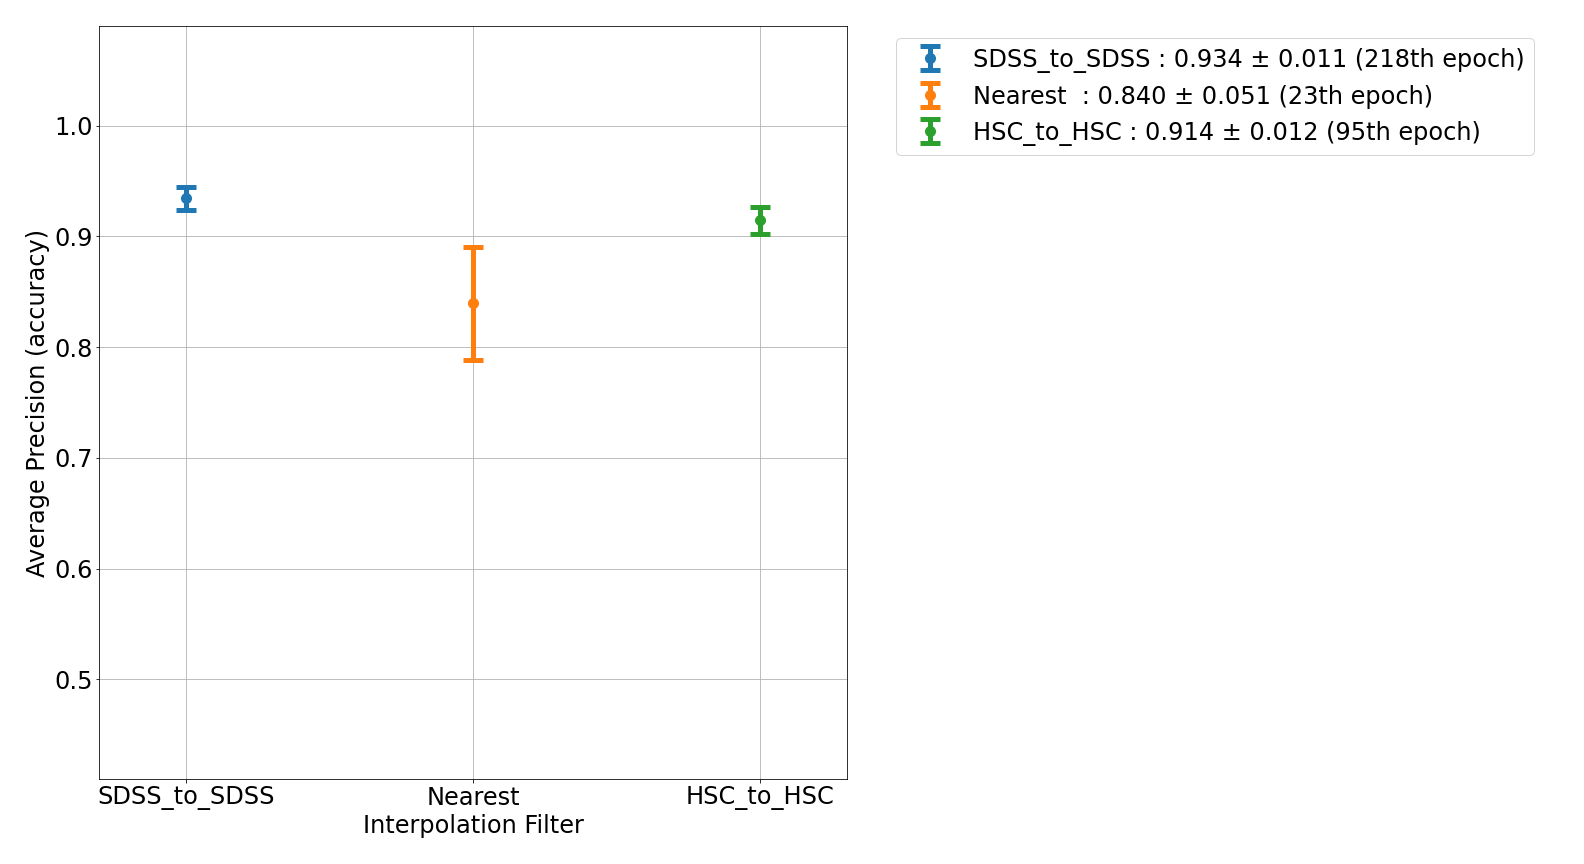
\includegraphics[width=1.0\hsize, keepaspectratio]{images/6syou/acc_with_errorbar_auto_epoch.png}
  \caption{3つの条件の分類モデルにおける,テストデータに対するaccuracy(1標準偏差)}
  \label{fig:6syou_zikkenn}
\end{figure}


\newpage
\chapter{おわりに}
本研究は,銀河画像データを用いて深層学習によって銀河形態を学習したモデルが,学習データに用いた画像よりも解像度の低い画像データに対し適用が行えるかについて検証した.具体的には,SDSSから取得した切り出し画像とそれを縮小した縮小画像を用意し,
学習データとテストデータとの間に画像解像度差がある場合にテストデータへの予測が成立するか,また学習データとテストデータとの間の解像度差がどれほどまでならば,学習データとテストデータの画像解像度が揃っている状況での予測結果と同程度の精度を達成するかを調べた.


その結果,学習データとテストデータとの間に1/4倍までの画像解像度差が生じていても,解像度差がない場合の予測精度であるaccuracy$0.917 \pm 0.020$と同程度の精度の予測を行うことに成功した.
この結果を受け,将来展望である「異なる観測装置データの組み合わせ」を実際に行い深層学習モデルの作成を行ったところ,
高解像度データのみで学習を行ったモデルのテストデータに対するaccuracyは$0.934 \pm 0.011$,低解像度データのみで学習を行ったモデルのテストデータに対するaccuracyは$0.914 \pm 0.012$であり,
結果として高解像度データのみで学習およびテストを行ったモデルと,低解像度データのみで学習およびテストを行ったモデルとの間で分類精度に有意な差が生じなかった.
この結果はTadaki et al.(2020)で示された結果と異なることから,本研究における将来展望は改善が望まれる.

今後の課題として,
\begin{inparaenum}[(1)]
 \item SDSSとGZを用いた深層学習銀河形態分類モデルの更なる精度向上
 \item 高空間解像度画像データ(HSC画像データ)を用いた深層学習モデルにおけるモデル改善
\end{inparaenum}
が必要である.
% END:本編----------------------------------------

% START:参考文献----------------------------------
%% ベタ打ちの場合
% \begin{thebibliography}{1}
% \bibitem{key1}サイト名\\ \url{http://google.com} (yyyy年mm月dd日アクセス) % ウェブサイトの場合
% \bibitem{key2}著者,書籍タイトル,出版                                      % 書籍,論文の場合
% \end{thebibliography}


%% bibtexを使用する場合
\newpage
\bibliography{Master_thesis_bib}         % .bibファイルから拡張子を外した名前 ex)ref.bib
\bibliographystyle{junsrt} % 参考文献出力スタイル
% \nocite{*}                 % 参照していない項目も出力する
% END:参考文献------------------------------------


\newpage
\chapter*{謝辞}
本研究を進めるにあたり,ご指導を頂いた新潟大学の飯田佑輔准教授および東京理科大学の大井渚様,そしてデータセット作成や宇宙関連知識取得に際し多大な助力をいただいた同研究室の津田様に,厚く感謝申し上げます.
また,日常の議論を通じて多くの知識や示唆を頂いた飯田研究室の皆様に感謝いたします.

SDSSおよびSDSS-IIの資金はアルフレッド・P・スローン財団から提供され,また参加機関は米国科学財団,米国エネルギー省,米国航空宇宙局,日本の文部科学省,マックスプランク協会,英国高等教育基金協会です.SDSSのWebサイトは,http://www.sdss.org/ です. 

SDSSは参加機関のための天体物理学研究コンソーシアムによって運営されています.参加機関は,アメリカ自然史博物館,ポツダム天体物理学研究所,バーゼル大学,ケンブリッジ大学,ケース・ウェスタン・リザーブ大学,シカゴ大学,ドレクセル大学,フェルミラボ社,高等研究所,日本参加グループ,ジョンズ・ホプキンス大学,原子核宇宙物理学合同研究所,カブリ粒子宇宙物理学研究所,韓国科学者グループ,中国科学者グループ,中国科学者グループ,韓国科学者グループ 韓国科学者グループ,中国科学院(LAMOST),ロスアラモス国立研究所,マックスプランク天文学研究所,マックスプランク天体物理学研究所,ニューメキシコ州立大学,オハイオ州立大学,ピッツバーグ大学,ポーツマス大学,プリンストン大学,米国海軍天文台,ワシントン大学です.

Galaxy Zooプロジェクトに参加し,形態分類カタログ作成を行ってくださったボランティアの方々に感謝いたします.Galaxy Zooに参加したボランティアの方々の一覧は,https://authors.gala\\xyzoo.org/authors.html\#galaxyzooにて参照することができます.

\end{document}
%------------------------------------------------
